\documentclass[a4paper,11pt,fleqn,dvipsnames,twoside,openright]{memoir} 	% Openright aabner kapitler paa hoejresider (openany begge)

%%%% PACKAGES %%%%

% ¤¤ Oversaettelse og tegnsaetning ¤¤ %
\usepackage[utf8]{inputenc}					% Input-indkodning af tegnsaet (UTF8)
\usepackage[danish]{babel}					% Dokumentets sprog
\usepackage[T1]{fontenc}					% Output-indkodning af tegnsaet (T1)
\usepackage{ragged2e,anyfontsize}			% Justering af elementer
\usepackage{fixltx2e}						% Retter forskellige fejl i LaTeX-kernen	

\usepackage[T1]{fontenc}					% Fixed scalable font problem jesper havde!
\usepackage{lmodern}						% Fixed scalable font problem jesper havde!
															
% ¤¤ Figurer og tabeller (floats) ¤¤ %
\usepackage{graphicx} 						% Haandtering af eksterne billeder (JPG, PNG, EPS, PDF)
%\usepackage{eso-pic}						% Tilfoej billedekommandoer paa hver side
%\usepackage{wrapfig}						% Indsaettelse af figurer omsvoebt af tekst. \begin{wrapfigure}{Placering}{Stoerrelse}
\usepackage{multirow}                		% Fletning af raekker og kolonner (\multicolumn og \multirow)
\usepackage{multicol}         	        	% Muliggoer output i spalter
\usepackage{rotating}						% Rotation af tekst med \begin{sideways}...\end{sideways}
\usepackage{colortbl} 						% Farver i tabeller (fx \columncolor og \rowcolor)
\usepackage{xcolor}							% Definer farver med \definecolor. Se mere: http://en.wikibooks.org/wiki/LaTeX/Colors
\usepackage{flafter}						% Soerger for at floats ikke optraeder i teksten foer deres reference
\let\newfloat\relax 						% Justering mellem float-pakken og memoir
\usepackage{float}							% Muliggoer eksakt placering af floats, f.eks. \begin{figure}[H]
\usepackage{longtable}
\usepackage[section]{placeins}
\usepackage{microtype}
\usepackage{listings}						% Kildekode formatering af udskrifter

% ¤¤ Matematik mm. ¤¤
\usepackage{amsmath,amssymb,stmaryrd} 		% Avancerede matematik-udvidelser
\usepackage{mathtools}						% Andre matematik- og tegnudvidelser
\usepackage{textcomp}                 		% Symbol-udvidelser (f.eks. promille-tegn med \textperthousand )
\usepackage{rsphrase}						% Kemi-pakke til RS-saetninger, f.eks. \rsphrase{R1}
\usepackage[version=3]{mhchem} 				% Kemi-pakke til flot og let notation af formler, f.eks. \ce{Fe2O3}
\usepackage{siunitx}						% Flot og konsistent praesentation af tal og enheder med \si{enhed} og \SI{tal}{enhed}
\sisetup{output-decimal-marker = {,}}		% Opsaetning af \SI (DE for komma som decimalseparator) 

% ¤¤ Referencer og kilder ¤¤ %
\usepackage[danish]{varioref}				% Muliggoer bl.a. krydshenvisninger med sidetal (\vref)
\usepackage{natbib}							% Udvidelse med naturvidenskabelige citationsmodeller
%\usepackage{xr}							% Referencer til eksternt dokument med \externaldocument{<NAVN>}
%\usepackage{glossaries}					% Terminologi- eller symbolliste (se mere i Daleifs Latex-bog)

% ¤¤ Misc. ¤¤ %
\usepackage{listings}						% Placer kildekode i dokumentet med \begin{lstlisting}...\end{lstlisting}
\usepackage{lipsum}							% Dummy text \lipsum[..]
\usepackage[shortlabels]{enumitem}			% Muliggoer enkelt konfiguration af lister
\usepackage{pdfpages}						% Goer det muligt at inkludere pdf-dokumenter med kommandoen \includepdf[pages={x-y}]{fil.pdf}	
\pdfoptionpdfminorversion=6					% Muliggoer inkludering af pdf dokumenter, af version 1.6 og hoejere
\pretolerance=1 							% Justering af afstand mellem ord (hoejt tal, mindre orddeling og mere luft mellem ord)
\hbadness=10000
\vbadness=10000

% Kommentarer og rettelser med \fxnote. Med 'final' i stedet for 'draft' udloeser hver note en error i den faerdige rapport.
\usepackage[footnote,draft,danish,silent,nomargin]{fixme}		


%%%% CUSTOM SETTINGS %%%%

% ¤¤ Marginer ¤¤ %
\setlrmarginsandblock{3.5cm}{2.5cm}{*}		% \setlrmarginsandblock{Indbinding}{Kant}{Ratio}
\setulmarginsandblock{2.5cm}{3.0cm}{*}		% \setulmarginsandblock{Top}{Bund}{Ratio}
\checkandfixthelayout 						% Oversaetter vaerdier til brug for andre pakker

%	¤¤ Afsnitsformatering ¤¤ %
\setlength{\parindent}{0mm}           		% Stoerrelse af indryk
\setlength{\parskip}{3mm}          			% Afstand mellem afsnit ved brug af double Enter
\linespread{1,1}							% Linie afstand

% ¤¤ Litteraturlisten ¤¤ %
\bibpunct[,]{[}{]}{;}{a}{,}{,} 				% Definerer de 6 parametre ved Harvard henvisning (bl.a. parantestype og seperatortegn)
\bibliographystyle{bibtex/harvard}			% Udseende af litteraturlisten.

% ¤¤ Indholdsfortegnelse ¤¤ %
\setsecnumdepth{subsection}		 			% Dybden af nummerede overkrifter (part/chapter/section/subsection)
\maxsecnumdepth{subsection}					% Dokumentklassens graense for nummereringsdybde
\settocdepth{subsection} 					% Dybden af indholdsfortegnelsen

% ¤¤ Lister ¤¤ %
\setlist{
  topsep=0pt,								% Vertikal afstand mellem tekst og listen
  itemsep=-1ex,								% Vertikal afstand mellem items
} 

% ¤¤ Visuelle referencer ¤¤ %
\usepackage[colorlinks]{hyperref}			% Danner klikbare referencer (hyperlinks) i dokumentet.
\hypersetup{colorlinks = true,				% Opsaetning af farvede hyperlinks (interne links, citeringer og URL)
    linkcolor = black,
    citecolor = black,
    urlcolor = black
}

% ¤¤ Opsaetning af figur- og tabeltekst ¤¤ %
\captionnamefont{\small\bfseries\itshape}	% Opsaetning af tekstdelen ('Figur' eller 'Tabel')
\captiontitlefont{\small}					% Opsaetning af nummerering
\captiondelim{. }							% Seperator mellem nummerering og figurtekst
\hangcaption								% Venstrejusterer flere-liniers figurtekst under hinanden
\captionwidth{\linewidth}					% Bredden af figurteksten
\setlength{\belowcaptionskip}{0pt}			% Afstand under figurteksten
		
% ¤¤ Opsaetning af listings ¤¤ %

\definecolor{commentGreen}{RGB}{34,139,24}
\definecolor{stringPurple}{RGB}{208,76,239}

\lstset{language=Matlab,					% Sprog
	basicstyle=\ttfamily\scriptsize,		% Opsaetning af teksten
	keywords={for,if,while,else,elseif,		% Noegleord at fremhaeve
			  end,break,return,case,
			  switch,function},
	keywordstyle=\color{blue},				% Opsaetning af noegleord
	commentstyle=\color{commentGreen},		% Opsaetning af kommentarer
	stringstyle=\color{stringPurple},		% Opsaetning af strenge
	showstringspaces=false,					% Mellemrum i strenge enten vist eller blanke
	numbers=left, numberstyle=\tiny,		% Linjenumre
	extendedchars=true, 					% Tillader specielle karakterer
	columns=flexible,						% Kolonnejustering
	breaklines, breakatwhitespace=true,		% Bryd lange linjer
}

% ¤¤ Navngivning ¤¤ %
\addto\captionsdanish{
	\renewcommand\appendixname{Appendiks}
	\renewcommand\contentsname{Indholdsfortegnelse}	
	\renewcommand\appendixpagename{Appendiks}
	\renewcommand\appendixtocname{Appendiks}
	\renewcommand\cftchaptername{\chaptername~}				% Skriver "Kapitel" foran kapitlerne i indholdsfortegnelsen
	\renewcommand\cftappendixname{\appendixname~}			% Skriver "Appendiks" foran appendiks i indholdsfortegnelsen
}

% ¤¤ Kapiteludssende ¤¤ %
\definecolor{numbercolor}{gray}{0.7}		% Definerer en farve til brug til kapiteludseende
\newif\ifchapternonum

\makechapterstyle{jenor}{					% Definerer kapiteludseende frem til ...
  \renewcommand\beforechapskip{0pt}
  \renewcommand\printchaptername{}
  \renewcommand\printchapternum{}
  \renewcommand\printchapternonum{\chapternonumtrue}
  \renewcommand\chaptitlefont{\fontfamily{pbk}\fontseries{db}\fontshape{n}\fontsize{25}{35}\selectfont\raggedleft}
  \renewcommand\chapnumfont{\fontfamily{pbk}\fontseries{m}\fontshape{n}\fontsize{1in}{0in}\selectfont\color{numbercolor}}
  \renewcommand\printchaptertitle[1]{%
    \noindent
    \ifchapternonum
    \begin{tabularx}{\textwidth}{X}
    {\let\\\newline\chaptitlefont ##1\par} 
    \end{tabularx}
    \par\vskip-2.5mm\hrule
    \else
    \begin{tabularx}{\textwidth}{Xl}
    {\parbox[b]{\linewidth}{\chaptitlefont ##1}} & \raisebox{-15pt}{\chapnumfont \thechapter}
    \end{tabularx}
    \par\vskip2mm\hrule
    \fi
  }
}											% ... her

\chapterstyle{jenor}						% Valg af kapiteludseende - Google 'memoir chapter styles' for alternativer

% ¤¤ Sidehoved ¤¤ %

\makepagestyle{IHA}							% Definerer sidehoved og sidefod udseende frem til ...
\makepsmarks{IHA}{%
	\createmark{chapter}{left}{shownumber}{}{. \ }
	\createmark{section}{right}{shownumber}{}{. \ }
	\createplainmark{toc}{both}{\contentsname}
	\createplainmark{lof}{both}{\listfigurename}
	\createplainmark{lot}{both}{\listtablename}
	\createplainmark{bib}{both}{\bibname}
	\createplainmark{index}{both}{\indexname}
	\createplainmark{glossary}{both}{\glossaryname}
}
\nouppercaseheads											% Ingen Caps oenskes

\makeevenhead{IHA}{Gruppe 3}{}{\leftmark}				% Definerer lige siders sidehoved (\makeevenhead{Navn}{Venstre}{Center}{Hoejre})
\makeoddhead{IHA}{\rightmark}{}{IHA - Aarhus Universitet}		% Definerer ulige siders sidehoved (\makeoddhead{Navn}{Venstre}{Center}{Hoejre})
\makeevenfoot{IHA}{\thepage}{}{}							% Definerer lige siders sidefod (\makeevenfoot{Navn}{Venstre}{Center}{Hoejre})
\makeoddfoot{IHA}{}{}{\thepage}								% Definerer ulige siders sidefod (\makeoddfoot{Navn}{Venstre}{Center}{Hoejre})
\makeheadrule{IHA}{\textwidth}{0.5pt}						% Tilfoejer en streg under sidehovedets indhold
\makefootrule{IHA}{\textwidth}{0.5pt}{1mm}					% Tilfoejer en streg under sidefodens indhold

\copypagestyle{IHAchap}{IHA}								% Sidehoved for kapitelsider defineres som standardsider, men med blank sidehoved
\makeoddhead{IHAchap}{}{}{}
\makeevenhead{IHAchap}{}{}{}
\makeheadrule{IHAchap}{\textwidth}{0pt}
\aliaspagestyle{chapter}{IHAchap}							% Den ny style vaelges til at gaelde for chapters
															% ... her
															
\pagestyle{IHA}												% Valg af sidehoved og sidefod


%%%% CUSTOM COMMANDS %%%%

% ¤¤ Billede hack ¤¤ %
\newcommand{\figur}[4]{
		\begin{figure}[H] \centering
			\includegraphics[width=#1\textwidth]{billeder/#2}
			\caption{#3}\label{#4}
		\end{figure} 
}

% ¤¤ Specielle tegn ¤¤ %
\newcommand{\decC}{^{\circ}\text{C}}
\newcommand{\dec}{^{\circ}}
\newcommand{\m}{\cdot}


%%%% ORDDELING %%%%

%%%% noget jesper har smidt ind %%%%
\hyphenation{}

\usepackage{graphicx}

\newcommand\xput[2][0.5]{%
    \rule{#1\linewidth}{0pt}\makebox[0pt][c]{#2}\hfill}
    


%%%% the end %%%%

\raggedbottom
\begin{document}

\include{filer/Underskrifter}

% Resume

% Resume

\chapter*{Resume}
Følgende rapport og tilhørende dokumentation beskriver arbejdet med gruppens semesterprojekt for 3. semester på Aarhus School of Engineering. Formålet med projektet er at afprøve de metoder og emner som semesterets fag har introduceret. Rapporten beskriver arbejdsmetoderne der er brugt fra idé til produkt, det egentlige produkt og udviklingen af dette samt de overvejelser og værktøjer som er benyttet. Dokumentationen indeholder en udtømmende teknisk beskrivelse af systemet.

Udgangspunktet for systemet er at kunne styre vanding af goldbaner på en nem og simpel måde. Fra et computerprogram kan en bruger styre systemets dele og fastlægge grænser for hvornår vanding skal starte mv. Autonome enheder placeres rundt på goldbanens huller og fra disse enheder distribueres et netværk af sensorer som overvåger de miljømæssige data.

Udviklingsforløbet er styret efter ASE-modellen, som er en halv-iterativ projektledelsesmetode. Produket er udviklet på to forskellige platforme. Brugerinteraktion sker igennem Devkit8000-platformen og det autonome system anvender PSoC4-boardet fra Cypress samt egen udviklet hardware til sensor-håndteringen. 

Projektet er endt ud i et funktionelt system som kan aflæse data fra sensorerne og reagerer på disse. Selve vand-pumpe-konstruktionen til vanding af banerne er kun lavet som en simpel konceptuel opstilling.

% English Abstract

% Abstract
\chapter*{Abstract}

The following document describes the work and process of the groups 3rd term project at Aarhus School of Engineering. The purpose of the project is to use and evaluate the methods and subjects taught at this terms courses. The report describes how the product came from an idea to a physical product as well as the details of the product and the methods used. The documentation holds all technical details about the product.

The product developed is an automatic watering system that helps controlling the environment around gold courses. From a computer program the user can control the whole system and set the limits from which the autonomous system reacts. The autonomous units are placed along the fairways with a grid of sensors placed in the ground on the fairway collecting environmental data.

Development is managed with the ASE-model, which is a semi-iterative project management process. Further more is it done on two different platforms namely the Devkit8000 for the user interaction component and the PSoC4 from Cypress as the core of the autonomous system along with specialised hardware for the sensors.

The results include a functional user interface and a fully established data-collection system. Though limited by the implementation of the water pump system, which is suppressed due time restrictions.

% Indledning

\tableofcontents*

Gruppen vil udvikle et system til vanding af golfbaner. I forbindelse med stigende temperaturer bliver det mere kritisk, at vandingen af golfbaner sker på de rigtige tidspunkter, for at holde banen spilbar. For at spare på ressourcerne er det også kritisk, ikke at spilde store mængder vand, på vanding af områder som ikke trænger til det. 

Med et system af intelligente enheder der arbejder autonomt, men som modtager indstillinger for vandingen fra en Master, styres vandingen på hele Golfbanen centralt. På denne måde sparer man arbejdstid for greenkeeperen og vandingen sker kun når det er nødvendigt. Systemet kaldes for EasyWater8000. 
Normalt vil man placere en af disse enheder ved hvert hul på golfbanen og lave et netværk af sensorer lokalt til denne enhed. Enheden kan herved overvåge området og vande hvis nødvendigt. Alle enhederne forbindes til et netværk, som er koblet sammen med en masterenhed. Grænseværdierne, for f.eks. jordfugtigheden, der afgør hvornår enheden, skal påbegynde vanding kommer fra Master og styres igennem denne af greenkeeperen. 


\begin{figure}[ht] \centering
\fbox{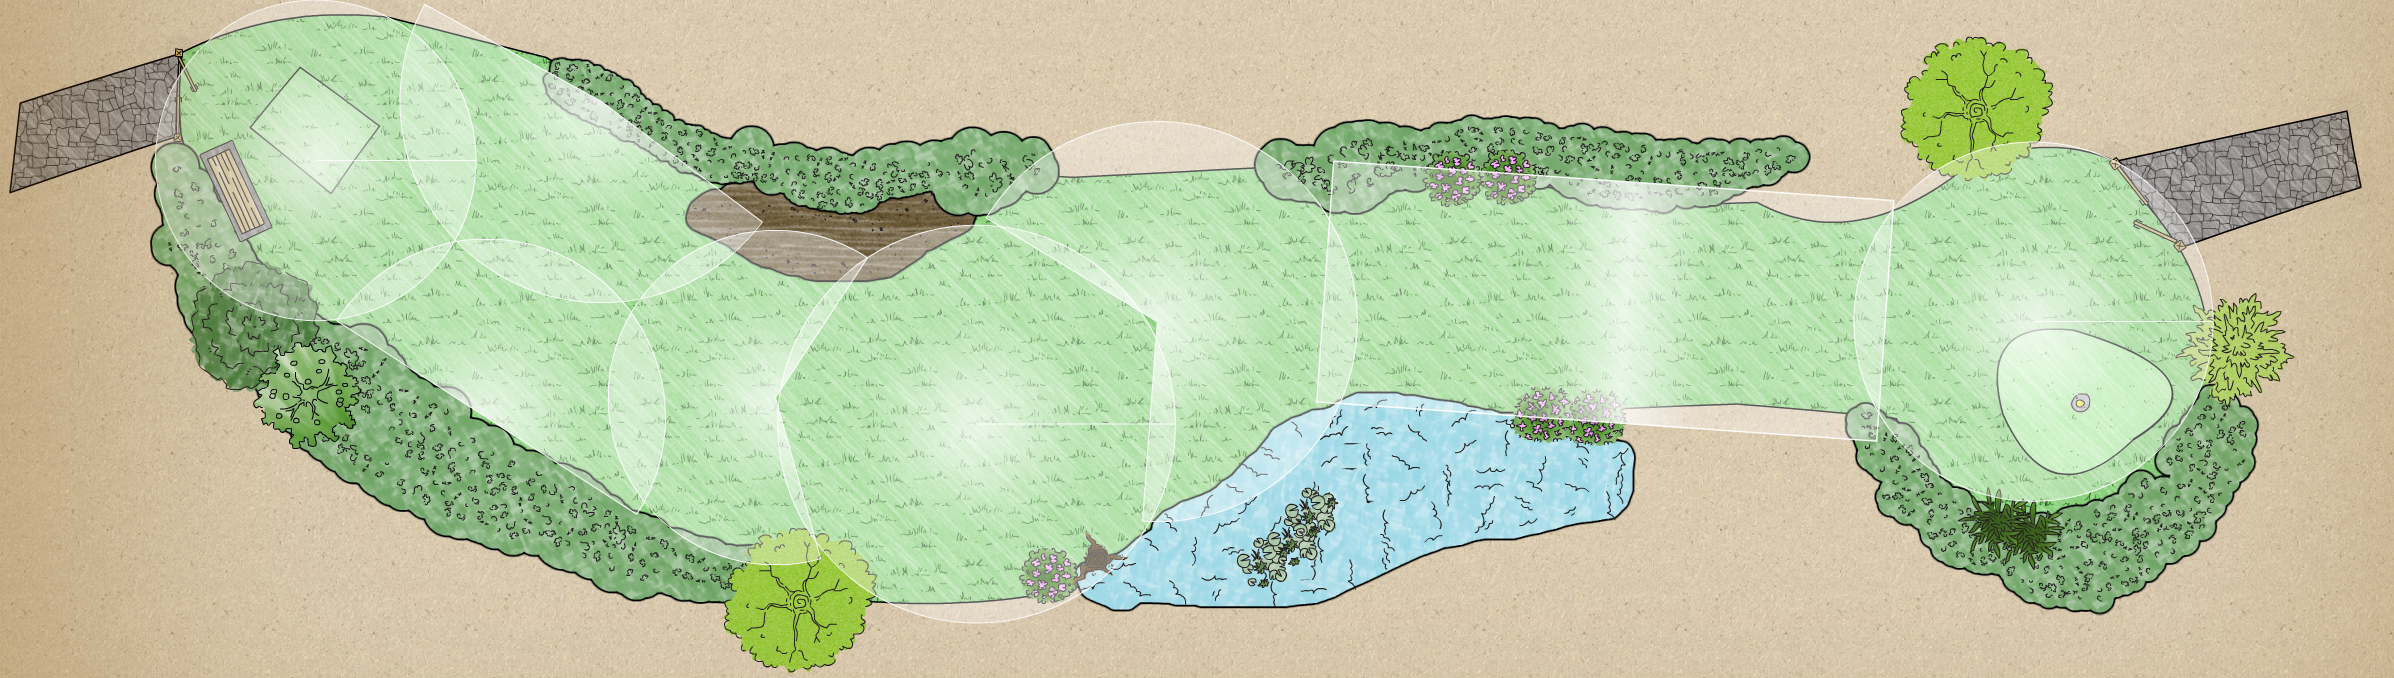
\includegraphics[height=4.1cm]{filer/indledning/billeder/hul_med_sprinkler}}
\caption{Overblik af golfhul med system}
\label{fig:systemoverblik}
\end{figure}

Figur \ref{fig:systemoverblik} illustrerer et hul på en given golfbane. Dette hul er inddelt i 11 områder, med hver sin sprinkler. Spinklere er markeret ved halv til helcirkler på figuren. Til venstre på figuren ses tee-stedet med tilhørende indgang. Ved denne indgang er der placeret en bevægelsessensor, som sørger for at der ikke kan vandes på banen, når der er spillere. 

Oversigt over blokkene i systemet kan ses i figur \ref{fig:bloksystemoverblik}. De tre hovedbegreber for systemet er Master, som er hovedenheden baseret på Devkit8000. Enhed som er de autonome undersystemer på hvert hul, hvor hovedenheden er PSoC, og Komponentpakker som er et begreb for pakken med temperatur- og fugtsensor samt sprinkler. Disse er distribueret ud på selve golfhullet.

\begin{figure}[ht] \centering
\fbox{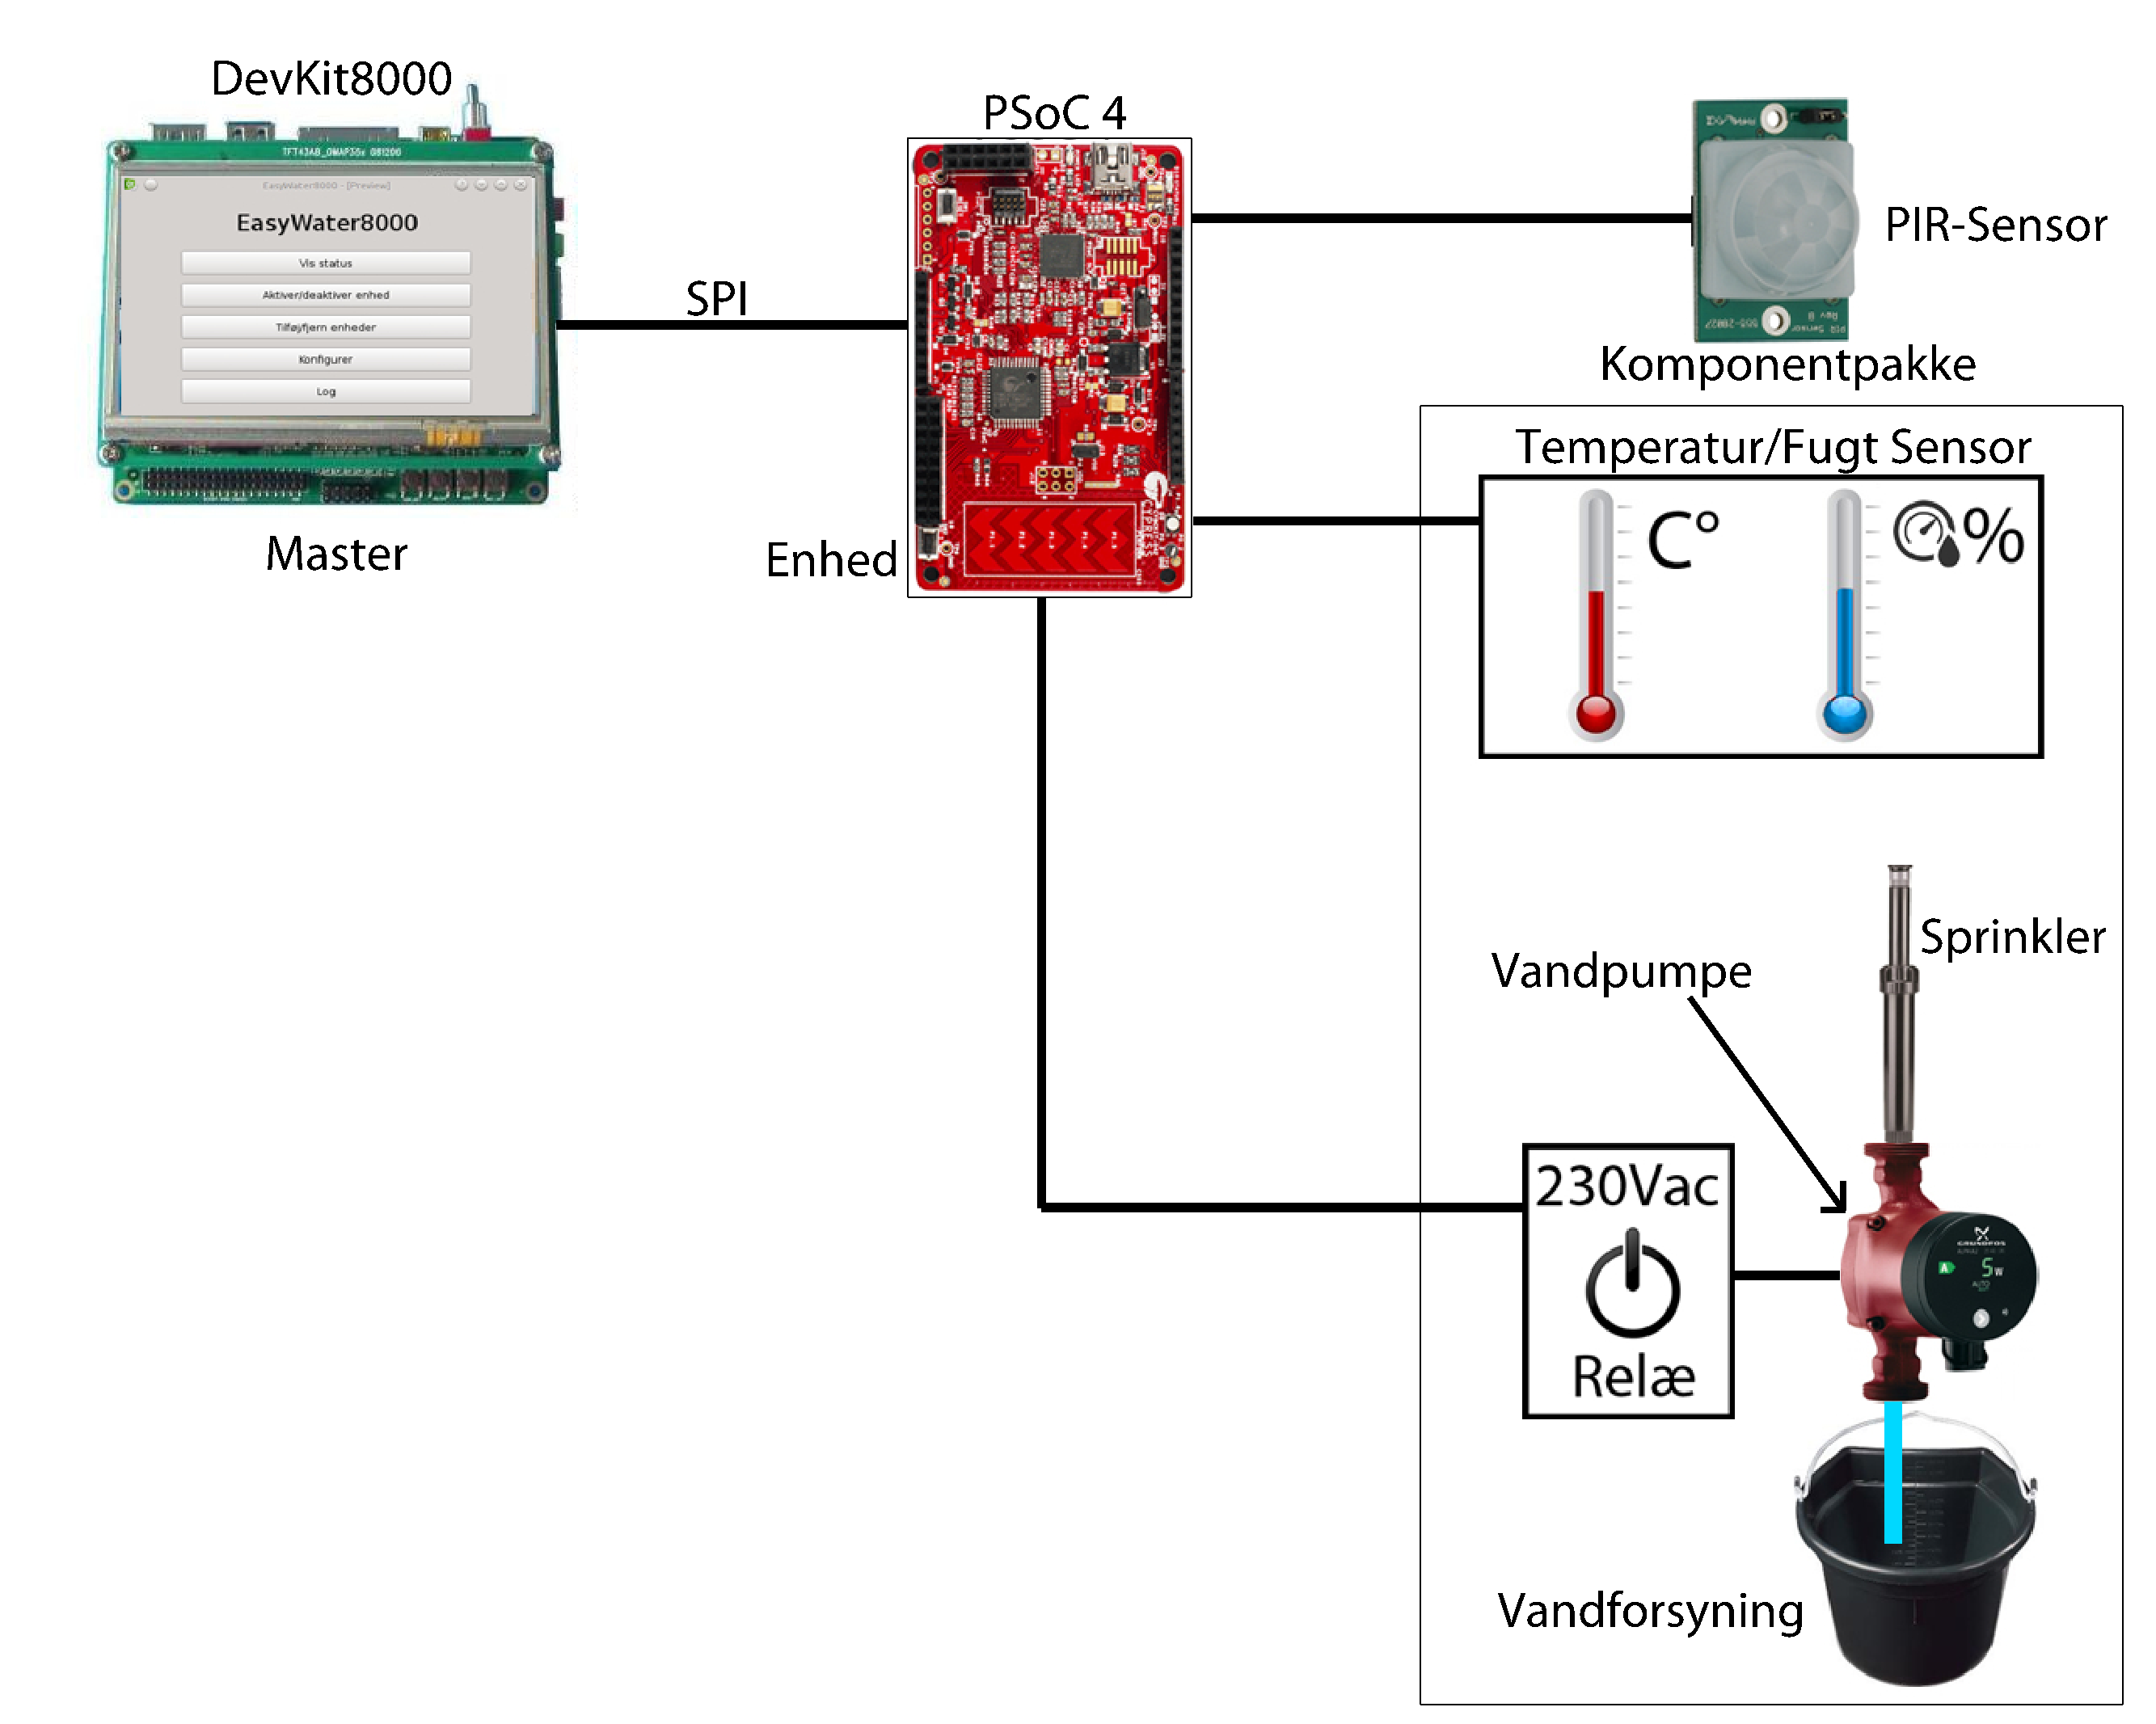
\includegraphics[height=10cm]{filer/indledning/billeder/vandingssystem}}
\caption{Systemoverblik}
\label{fig:bloksystemoverblik}
\end{figure}

En Enhed består altså af:
\begin{enumerate}
\item Fugtighedssensor(er)
\item Temperatursensor(er)
\item Bevægelsessensor(er) 
\item Sprinkler(e)
\item PSoC controller board
\end{enumerate}

Fugt- og temperatursensorerne registrerer banens behov for vanding. Bevægelsessensoren registrerer om der er spillere på det pågældende hul. Sprinkleren sørger for vandingen når der skal vandes. Denne skjules nede i græsset og kommer op når vandingen skal være aktiv.
PSoC4 controller-boardet bliver hjernen i Enheden. Denne holder styr på de generelle funktioner for Enheden så som udlæsning af data, aktivering af sprinkler m.v.

% Opgave formulering

\chapter{Opgaveformulering (MK PO)}

Konstruer et system til vanding af golfbaner. Systemet skal indeholde én Master (Devkit8000) som kontrollerer et netværk af Enheder (PSoC4). Kommunikationen imellem Master og Enhed skal foregå via den serielle kommunikation kaldet SPI. Via denne kommunikation skal Masteren kunne kontrollere de enkelte Enheder, samt indhente log-data fra disse. 
Enheden skal fungere autonomt, når denne er aktiveret. Enheden  er tilkoblet en komponentpakke bestående af fugt- og temperatursensor samt sprinkler med tilhørende pumpe og vandforsyning. Enheden skal således selv styre vanding af trængende områder. En bevægelsessensor skal placeres ved indgangen til hvert golfhul, hvis der registreres bevægelse blokeres en evt. vanding i 30 minutter.  

Figur \ref{fig:systemoversigt} illustrerer ovenstående.  

%SYSTEMOVERBLIK BILLEDE
\begin{figure}[h]
  \centering
    \includegraphics[width=\textwidth]{Billeder/Oversigt over EasyWater8000 og forbindelser mellem delsystemer}
    \caption{Systemoversigt}
    \label{fig:systemoversigt}
\end{figure}


% Afgrænsniger i projektet

\chapter{Projektafgrænsning (JS)}
%afgrænsninger i projektet her.

Et fuldt integreret vandingssystem er, grundet manglende ressourcer og tid, ikke en mulighed på dette semesterprojekt, men der udarbejdes i stedet en skaleret prototype.
Foruden størrelsesbegrænsning er der fra skolens side givet forbud mod, uanset tidligere baggrund, at der arbejdes på 230 VAC. Men da der indgår en 230 VAC pumpe i projektet har skolen givet særtilladelse til at der laves et relæ-kredsløb i en lukket kasse, hvori alle ledende dele er helt afskærmet for fysisk kontakt som kan ses på figur \ref{lab:230Vrelay}.

Hurtigt i projektets forløb fik vi tildelt en pumpe fra Grundfos, det viste sig senere at denne ikke kunne bruges til det ønskede formål med at skabe et vandtryk, da denne er en cirkulationspumpe. 

%Løsningen på dette ender med en billig vandpumpe til påmontering på en 230 V %boremaskine. 

\begin{figure}[H]
  \centering
    \includegraphics[width=0.75\textwidth]{Billeder/230Vrelay}
    \caption{Relæ i afskærmet kasse}
    \label{lab:230Vrelay}
\end{figure}

Efter at den serielle kommunikation (SPI) var implementeret færdig og klar til test, viste det sig at overførelsesafstanden på 22 cm, som først var tiltænkt, ikke kunne lade sig gøre, da dataen blev korrupt undervejs. Denne afstand blev da nedsat til 7 cm for at kunne overføre data uden fejl.
 
I softwareimplementeringen er der tiltænkt en  avanceret fejl-håndtering og filstruktur til at gemme opsætning- og logdata på Devkit8000. På grund af at vi mistede en software-mand i gruppen er disse ting udeladt til fordel for at få den grafiske brugerflade og den autonome funktionalitet op at køre. Dette har resulteret i at alle fejlbeskeder på den grafiske brugerflade ikke er implementeret.

Prototypen udvikles med nogle andre tidsintervaller end dem specificeret i kravspecifikationen. Dette skyldes at vi gerne vil kunne se systemet virke i lille skala og i test øjemed.

Tiderne er som følger.

\begin{itemize}
	\item Datalogning fra Enheder på Master hvert 15. sekund
	\item Datalogning og autonom reaktion på Enheder hvert 8. sekund
	\item Afbrydelse af autonomt system ifm. bevægelse: 20 sekunder
\end{itemize}

% Systembeskrivelse

\chapter{Systembeskrivelse (MK PO)}

EasyWater8000 er et samlet vandingssystem, hovedsagligt målrettet imod vanding af en golfbane. Her følger en detaljeret beskrivelse af systemet.

\begin{figure}[H]
  \centering
    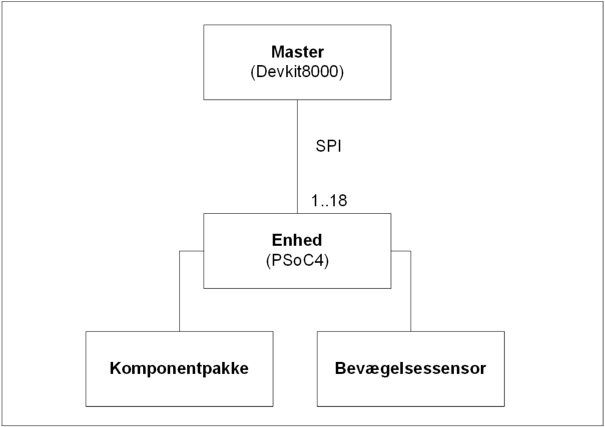
\includegraphics[width=0.9\textwidth]{billeder/systembeskrivelse}
    \caption{Oversigt over det samlede system}
    \label{fig:systembeskrivelse}
\end{figure}

Figur \ref{fig:systembeskrivelse} viser et simplificeret overblik over hvad EasyWater8000 består af. Der er en Master, som er hovedcomputeren i systemet med Linux (Angstrom) som styresystem. Masteren kommunikerer og styrer op til 18 Enheder der hver har en komponentpakke og en bevægelsessensor tilsluttet.

Komponentpakken er en samling af 3 komponenter, en temperatursensor og en fugtsensor til at hhv. måle temperaturen og fugtigheden i jorden omkring komponentpakken, samt en sprinkler til at vande græsset og jorden i samme område.

Bevægelsessensoren sidder ved hvert teested på golfbanen, og registrerer bevægelse i det område. Når der bliver registreret bevægelse vil sensoren give signal til at deaktivere vandingen på det givne golfhul, så golfspillerne ikke bliver utilsigtet våde.

Et golfhul kunne se ud som på Figur \ref{fig:hul_med_sprinkler}

\begin{figure}[H]
  \centering
    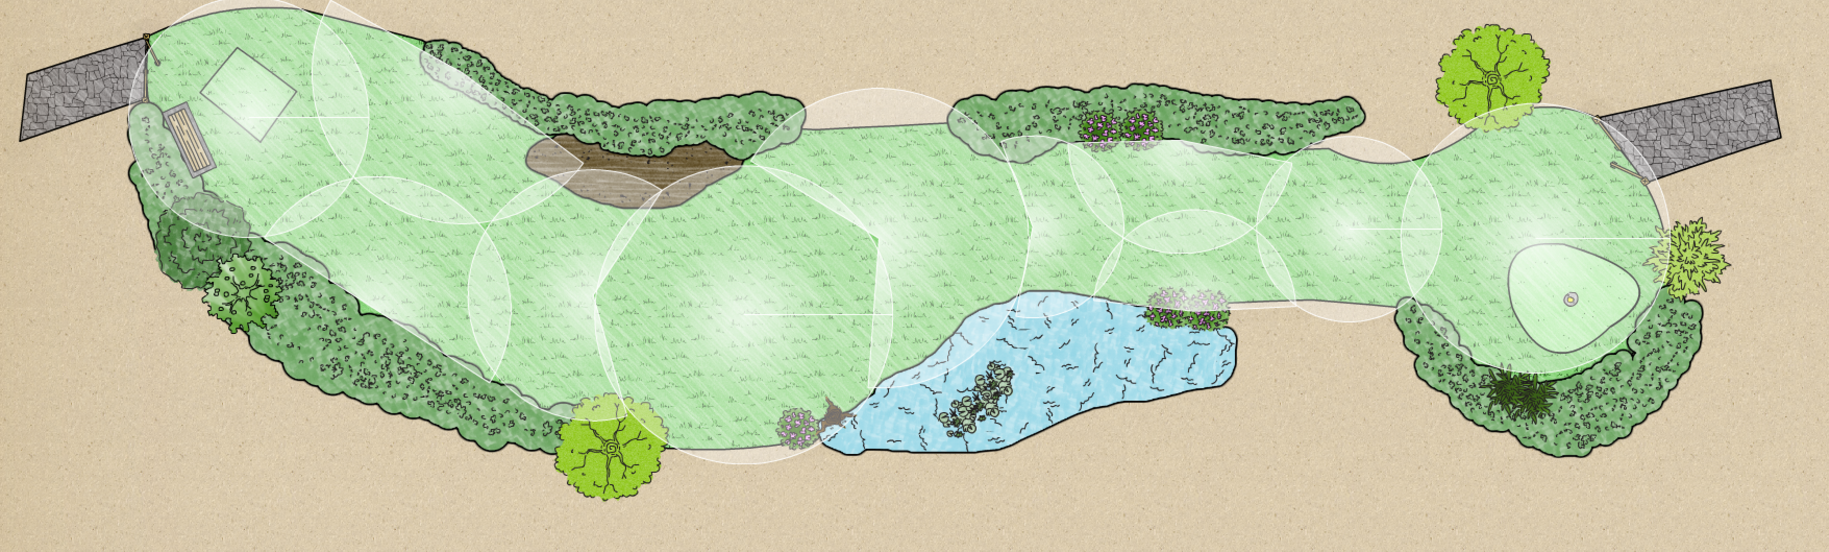
\includegraphics[width=\textwidth]{billeder/hul_med_sprinkler}
    \caption{Eksempel på golfbane med sprinklere}
    \label{fig:hul_med_sprinkler}
\end{figure}

Enhederne kører autonomt, dvs. de selv monitorerer fugt og temperatur og vander hvis grænserne overskrides. Enhederne får deres grænseværdier fra Masteren og logger sine målte data til Masteren, via SPI-kommunikation.

% Kravspec

\chapter{Krav}
EasyWater8000 er et system udviklet med henblik på at lette en greenkeepers opgave med at holde græsset på golfbanen. 	Systemet skal automatisk tænde for sprinklerne på golfbanen når den bliver for tør. Dette gør at greenkeeperen ikke selv skal tænde for det eller sætte faste vandetidspunkter, men at græsset bliver vandet når det har brug for det. Systemet måler både fugt og temperatur, al data samles i en log som kan printes på styringen (Masteren).  Desuden observerer systemet om en person eller spiller går ind på banen og deaktiverer vandingssystemet i en periode for systemet ikke vander hullet mens spilleren er derpå. 

Greenkeeperen kan fra styringen sætte en række værdier for hvor tørt og varmt der skal være før der vandes. Når værdierne er sat kan systemet køre af sig selv. Greenkeeperen kan også tvinge en vanding igennem hvis der f.eks. er en konkurrence næste dag og golfbanen således ikke vandes hele dage da der er personer derpå hele tiden. 

% generelle krav for systemet 

\chapter{Kravspecifikation}

% Indledning
\section{Indledning}
Gruppen vil udvikle et system til vanding af golfbaner. I forbindelse med stigende temperaturer bliver det mere kritisk, at vandingen af golfbaner sker på de rigtige tidspunkter, for at holde banen spilbar. For at spare på ressourcerne er det også kritisk, ikke at spilde store mængder vand, på vanding af områder som ikke trænger til det. 

Med et system af intelligente enheder der arbejder autonomt, men som modtager indstillinger for vandingen fra en Master, styres vandingen på hele Golfbanen centralt. På denne måde sparer man arbejdstid for greenkeeperen og vandingen sker kun når det er nødvendigt. Systemet kaldes for EasyWater8000. 
Normalt vil man placere en af disse enheder ved hvert hul på golfbanen og lave et netværk af sensorer lokalt til denne enhed. Enheden kan herved overvåge området og vande hvis nødvendigt. Alle enhederne forbindes til et netværk, som er koblet sammen med en masterenhed. Grænseværdierne, for f.eks. jordfugtigheden, der afgør hvornår enheden, skal påbegynde vanding kommer fra Master og styres igennem denne af greenkeeperen. 


\begin{figure}[ht] \centering
\fbox{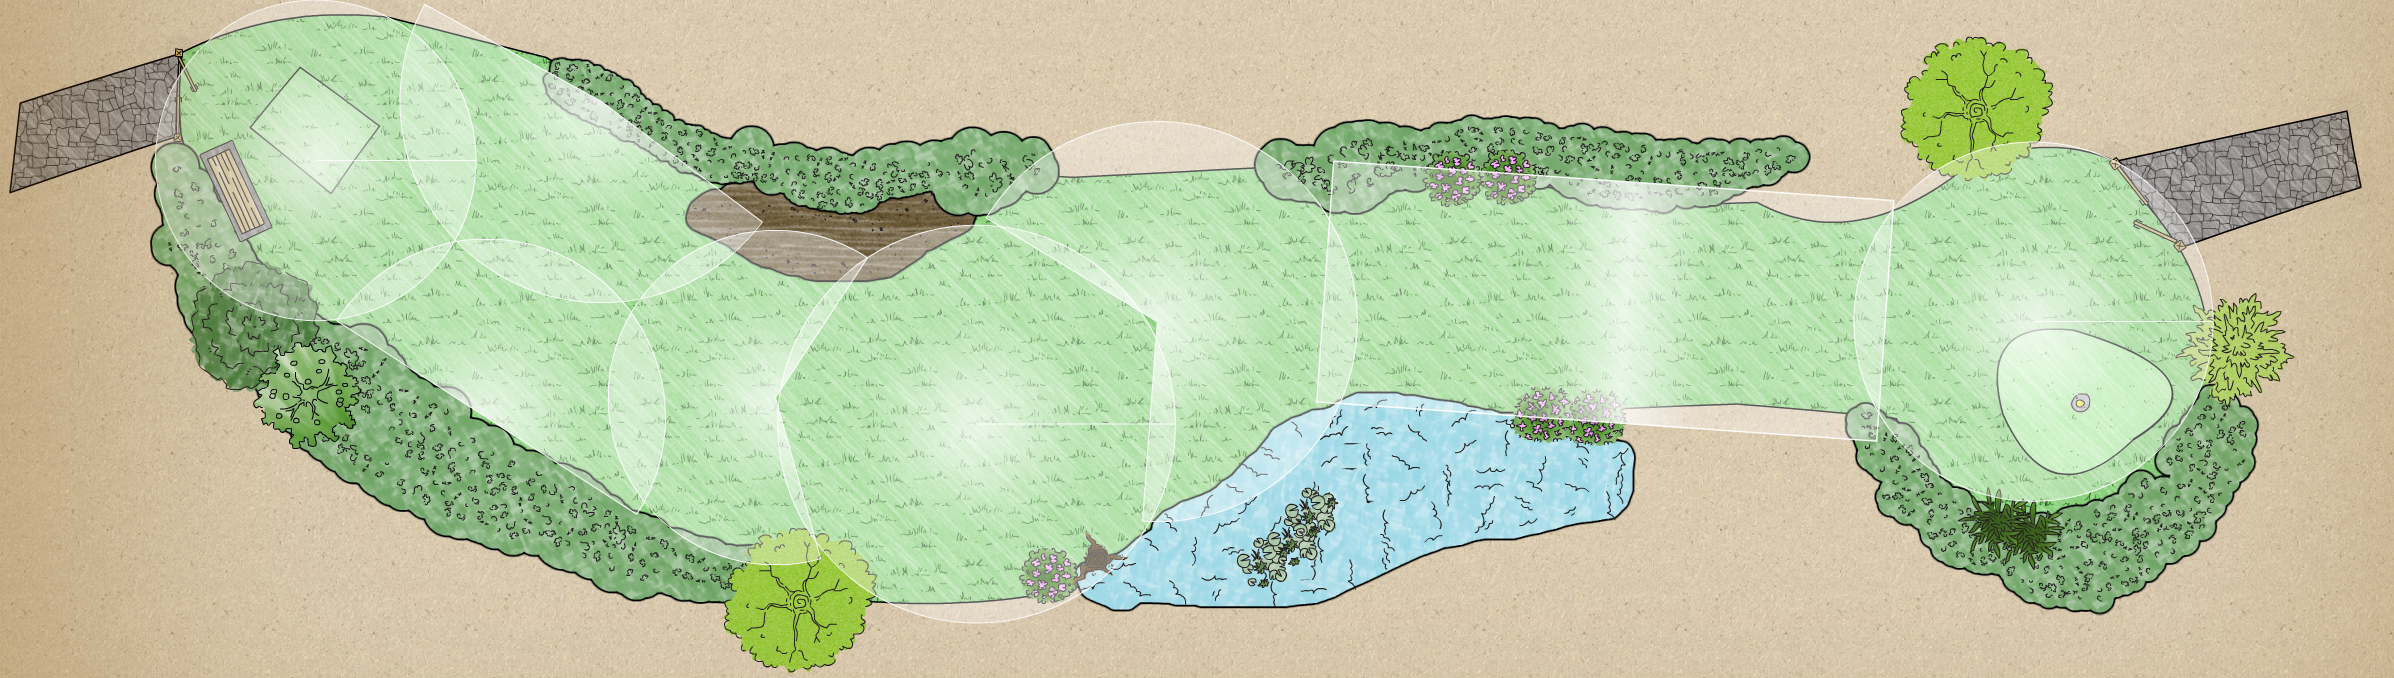
\includegraphics[height=4.1cm]{filer/indledning/billeder/hul_med_sprinkler}}
\caption{Overblik af golfhul med system}
\label{fig:systemoverblik}
\end{figure}

Figur \ref{fig:systemoverblik} illustrerer et hul på en given golfbane. Dette hul er inddelt i 11 områder, med hver sin sprinkler. Spinklere er markeret ved halv til helcirkler på figuren. Til venstre på figuren ses tee-stedet med tilhørende indgang. Ved denne indgang er der placeret en bevægelsessensor, som sørger for at der ikke kan vandes på banen, når der er spillere. 

Oversigt over blokkene i systemet kan ses i figur \ref{fig:bloksystemoverblik}. De tre hovedbegreber for systemet er Master, som er hovedenheden baseret på Devkit8000. Enhed som er de autonome undersystemer på hvert hul, hvor hovedenheden er PSoC, og Komponentpakker som er et begreb for pakken med temperatur- og fugtsensor samt sprinkler. Disse er distribueret ud på selve golfhullet.

\begin{figure}[ht] \centering
\fbox{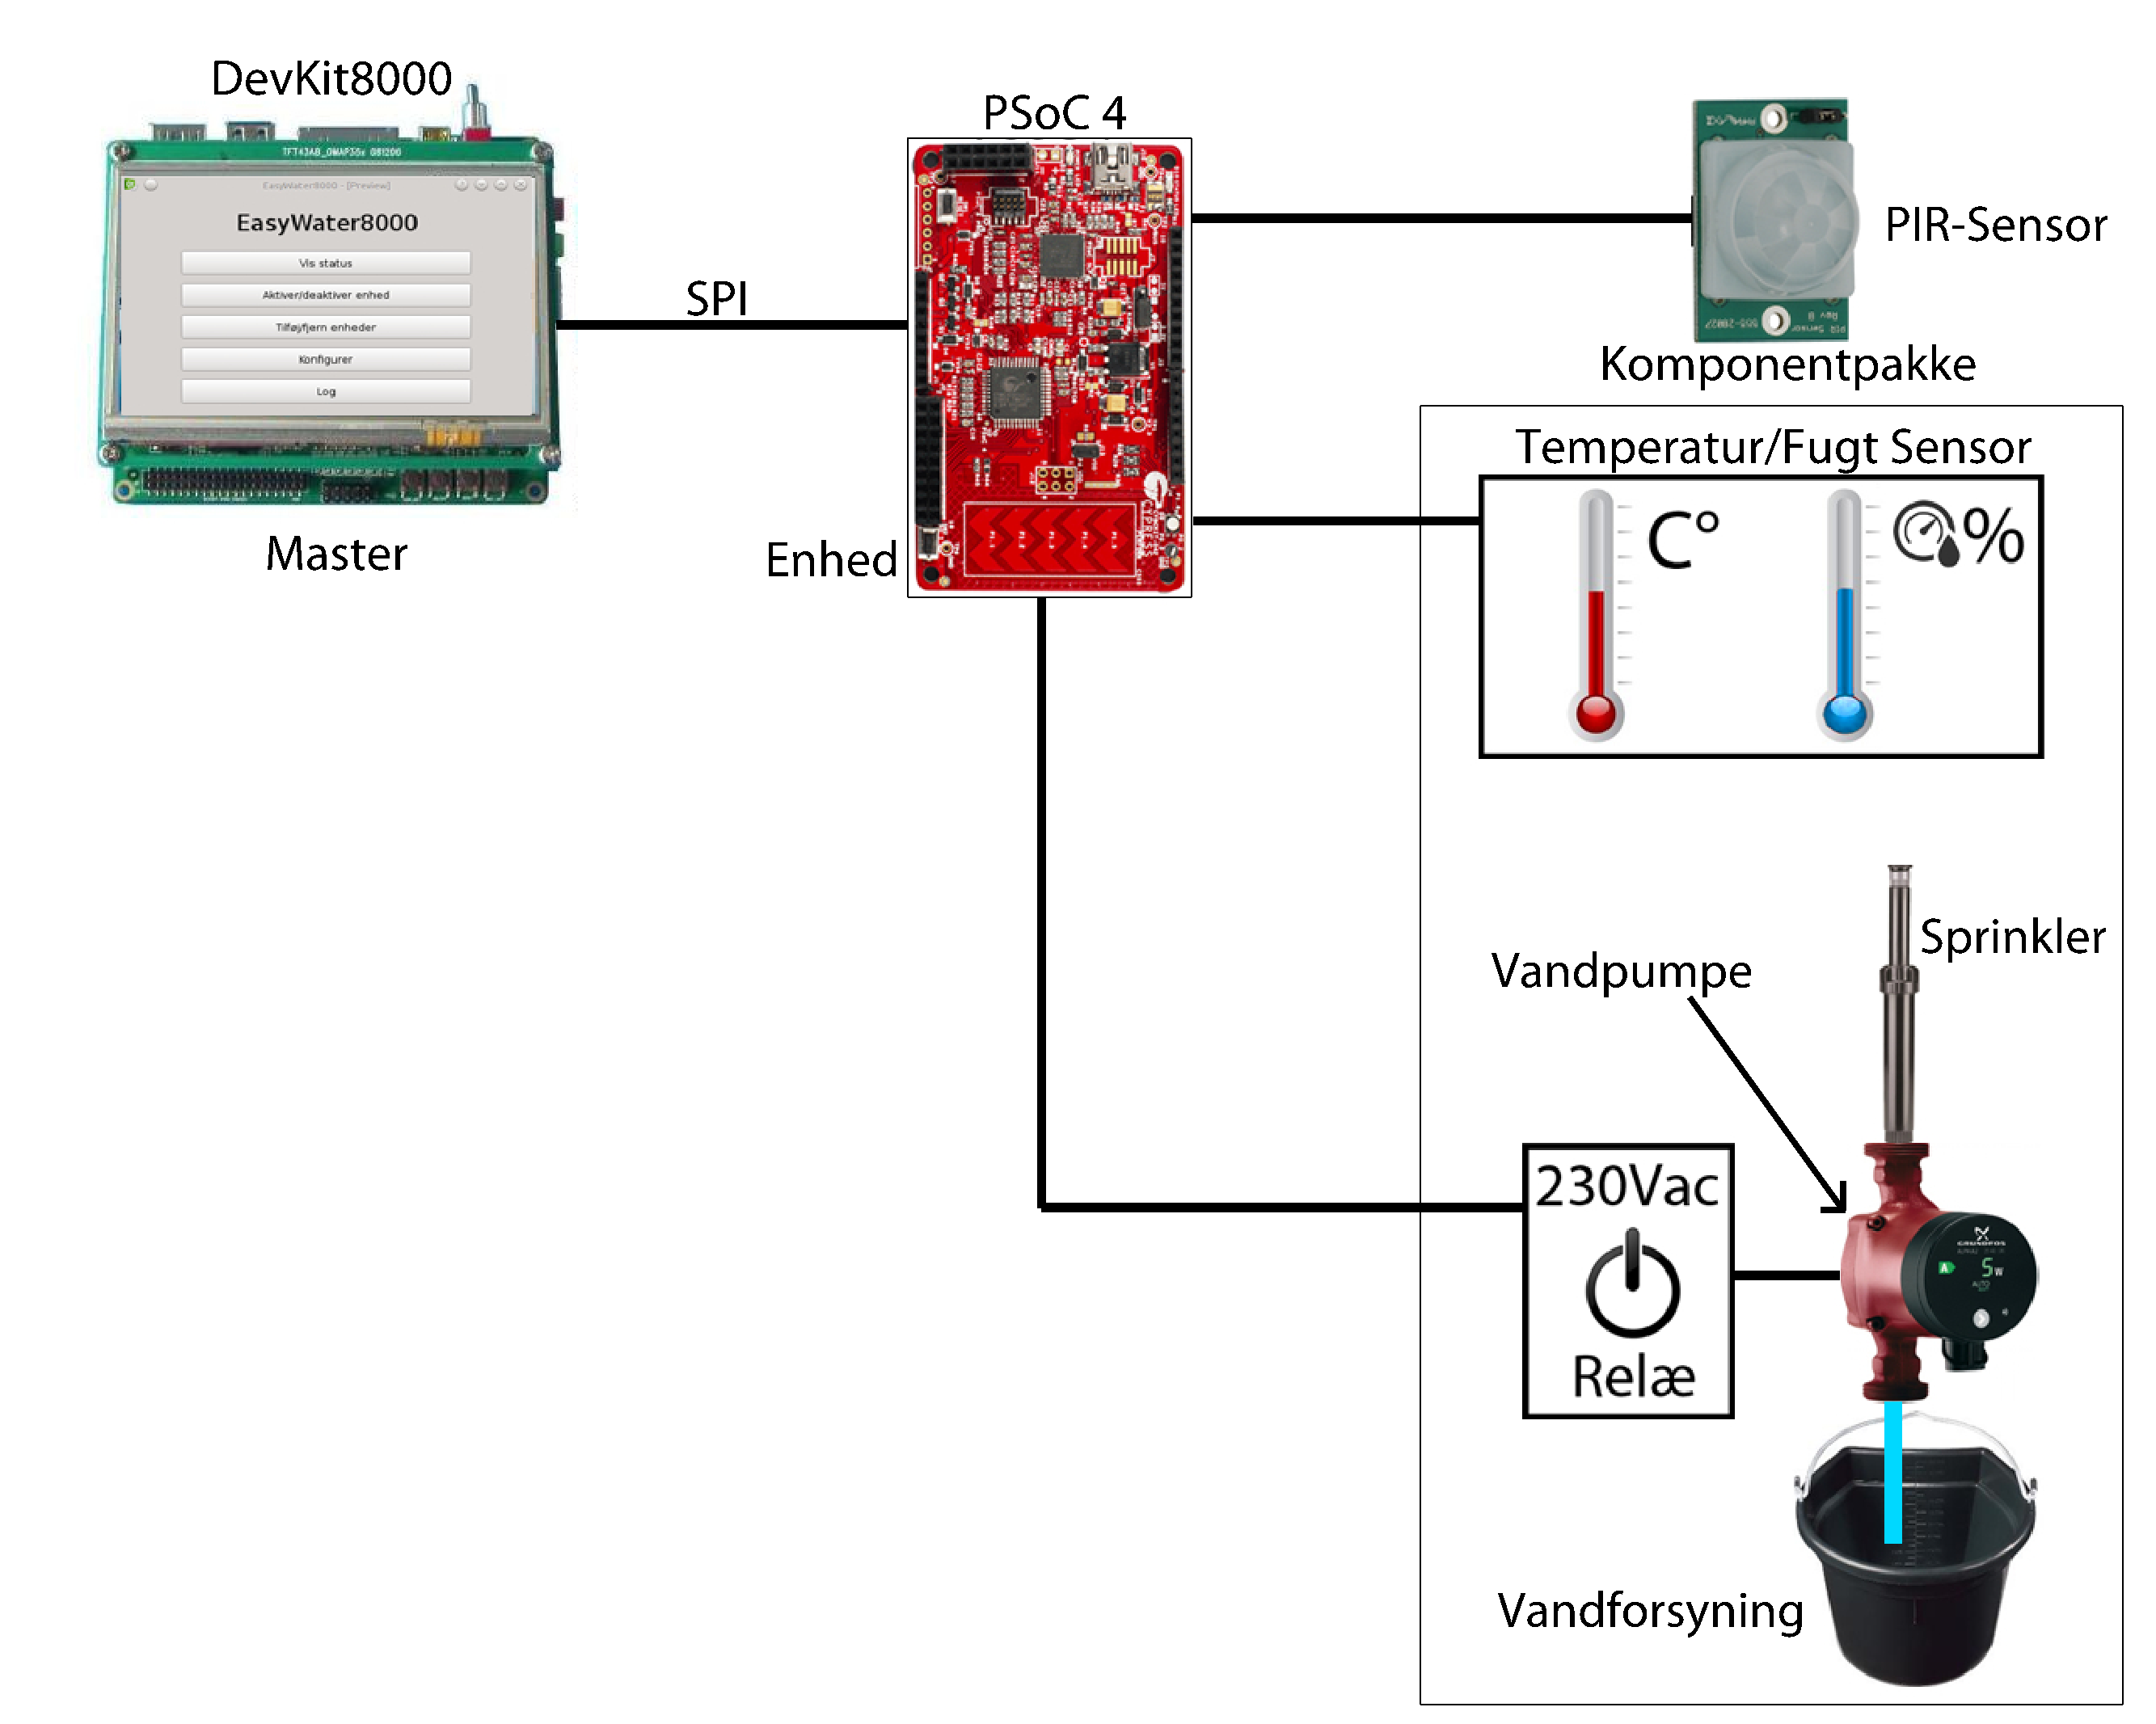
\includegraphics[height=10cm]{filer/indledning/billeder/vandingssystem}}
\caption{Systemoverblik}
\label{fig:bloksystemoverblik}
\end{figure}

En Enhed består altså af:
\begin{enumerate}
\item Fugtighedssensor(er)
\item Temperatursensor(er)
\item Bevægelsessensor(er) 
\item Sprinkler(e)
\item PSoC controller board
\end{enumerate}

Fugt- og temperatursensorerne registrerer banens behov for vanding. Bevægelsessensoren registrerer om der er spillere på det pågældende hul. Sprinkleren sørger for vandingen når der skal vandes. Denne skjules nede i græsset og kommer op når vandingen skal være aktiv.
PSoC4 controller-boardet bliver hjernen i Enheden. Denne holder styr på de generelle funktioner for Enheden så som udlæsning af data, aktivering af sprinkler m.v.

% Aktører
\newpage
\section{Aktører}
Her beskrives systemets aktører. Disse vil blive refereret til, i de efterfølgende usecase-beskrivelser.


%% !!! Aktør kontekst diagram !!!
\begin{figure}[htbp] \centering
\fbox{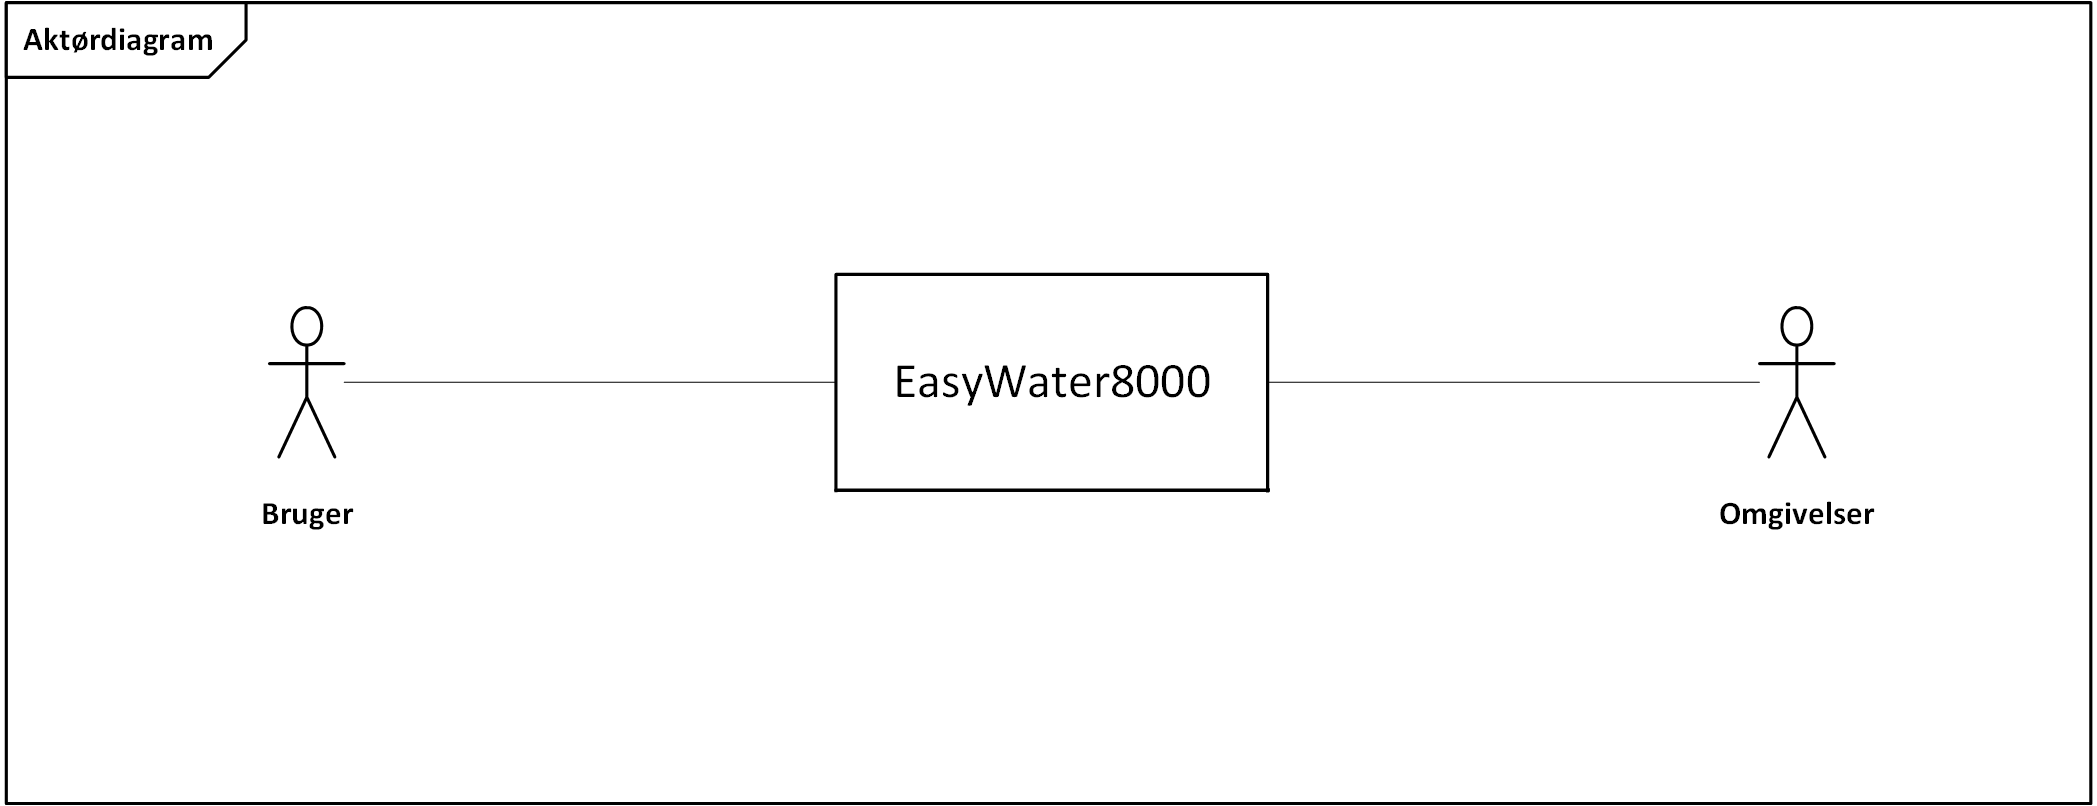
\includegraphics[width=0.9\textwidth]{filer/kravspec/visio/Kontekst_Diagram}}
\caption{Kontekst diagram}
\label{lab:kontekstdiagram}
\end{figure}

\begin{table}[!htbp] \centering
	\begin{tabular}{|p{2.5cm}|p{11.5cm}|}
	\hline
		\textbf{Aktør navn} & \textbf{Beskrivelse} \\\hline
		Bruger & Bruger-aktøren vil normalt være greenkeeperen. Det er vedkommende som kontrollerer og betjener systemet. (Primær) \\\hline

		Golfbane & De almene omgivelser på golfbanen, som har indflydelse på systemets sensorer. Det indebærer temperatur, fugtighed og bevægelser i områderne omkring systemet. (Sekundær) \\\hline
	\end{tabular}
\end{table}



% Usecases
\newpage
\section{Usecases}\label{header:usecases}

Her følger en dybere beskrivelse af systemets opbygning og måde at virke på. Dette gøres med fulde usecase-beskrivelser hvor systemets virkning er beskrevet i detaljer.

%% !!! Use case diagram !!!
\begin{figure}[H] \centering
\vspace*{\fill}
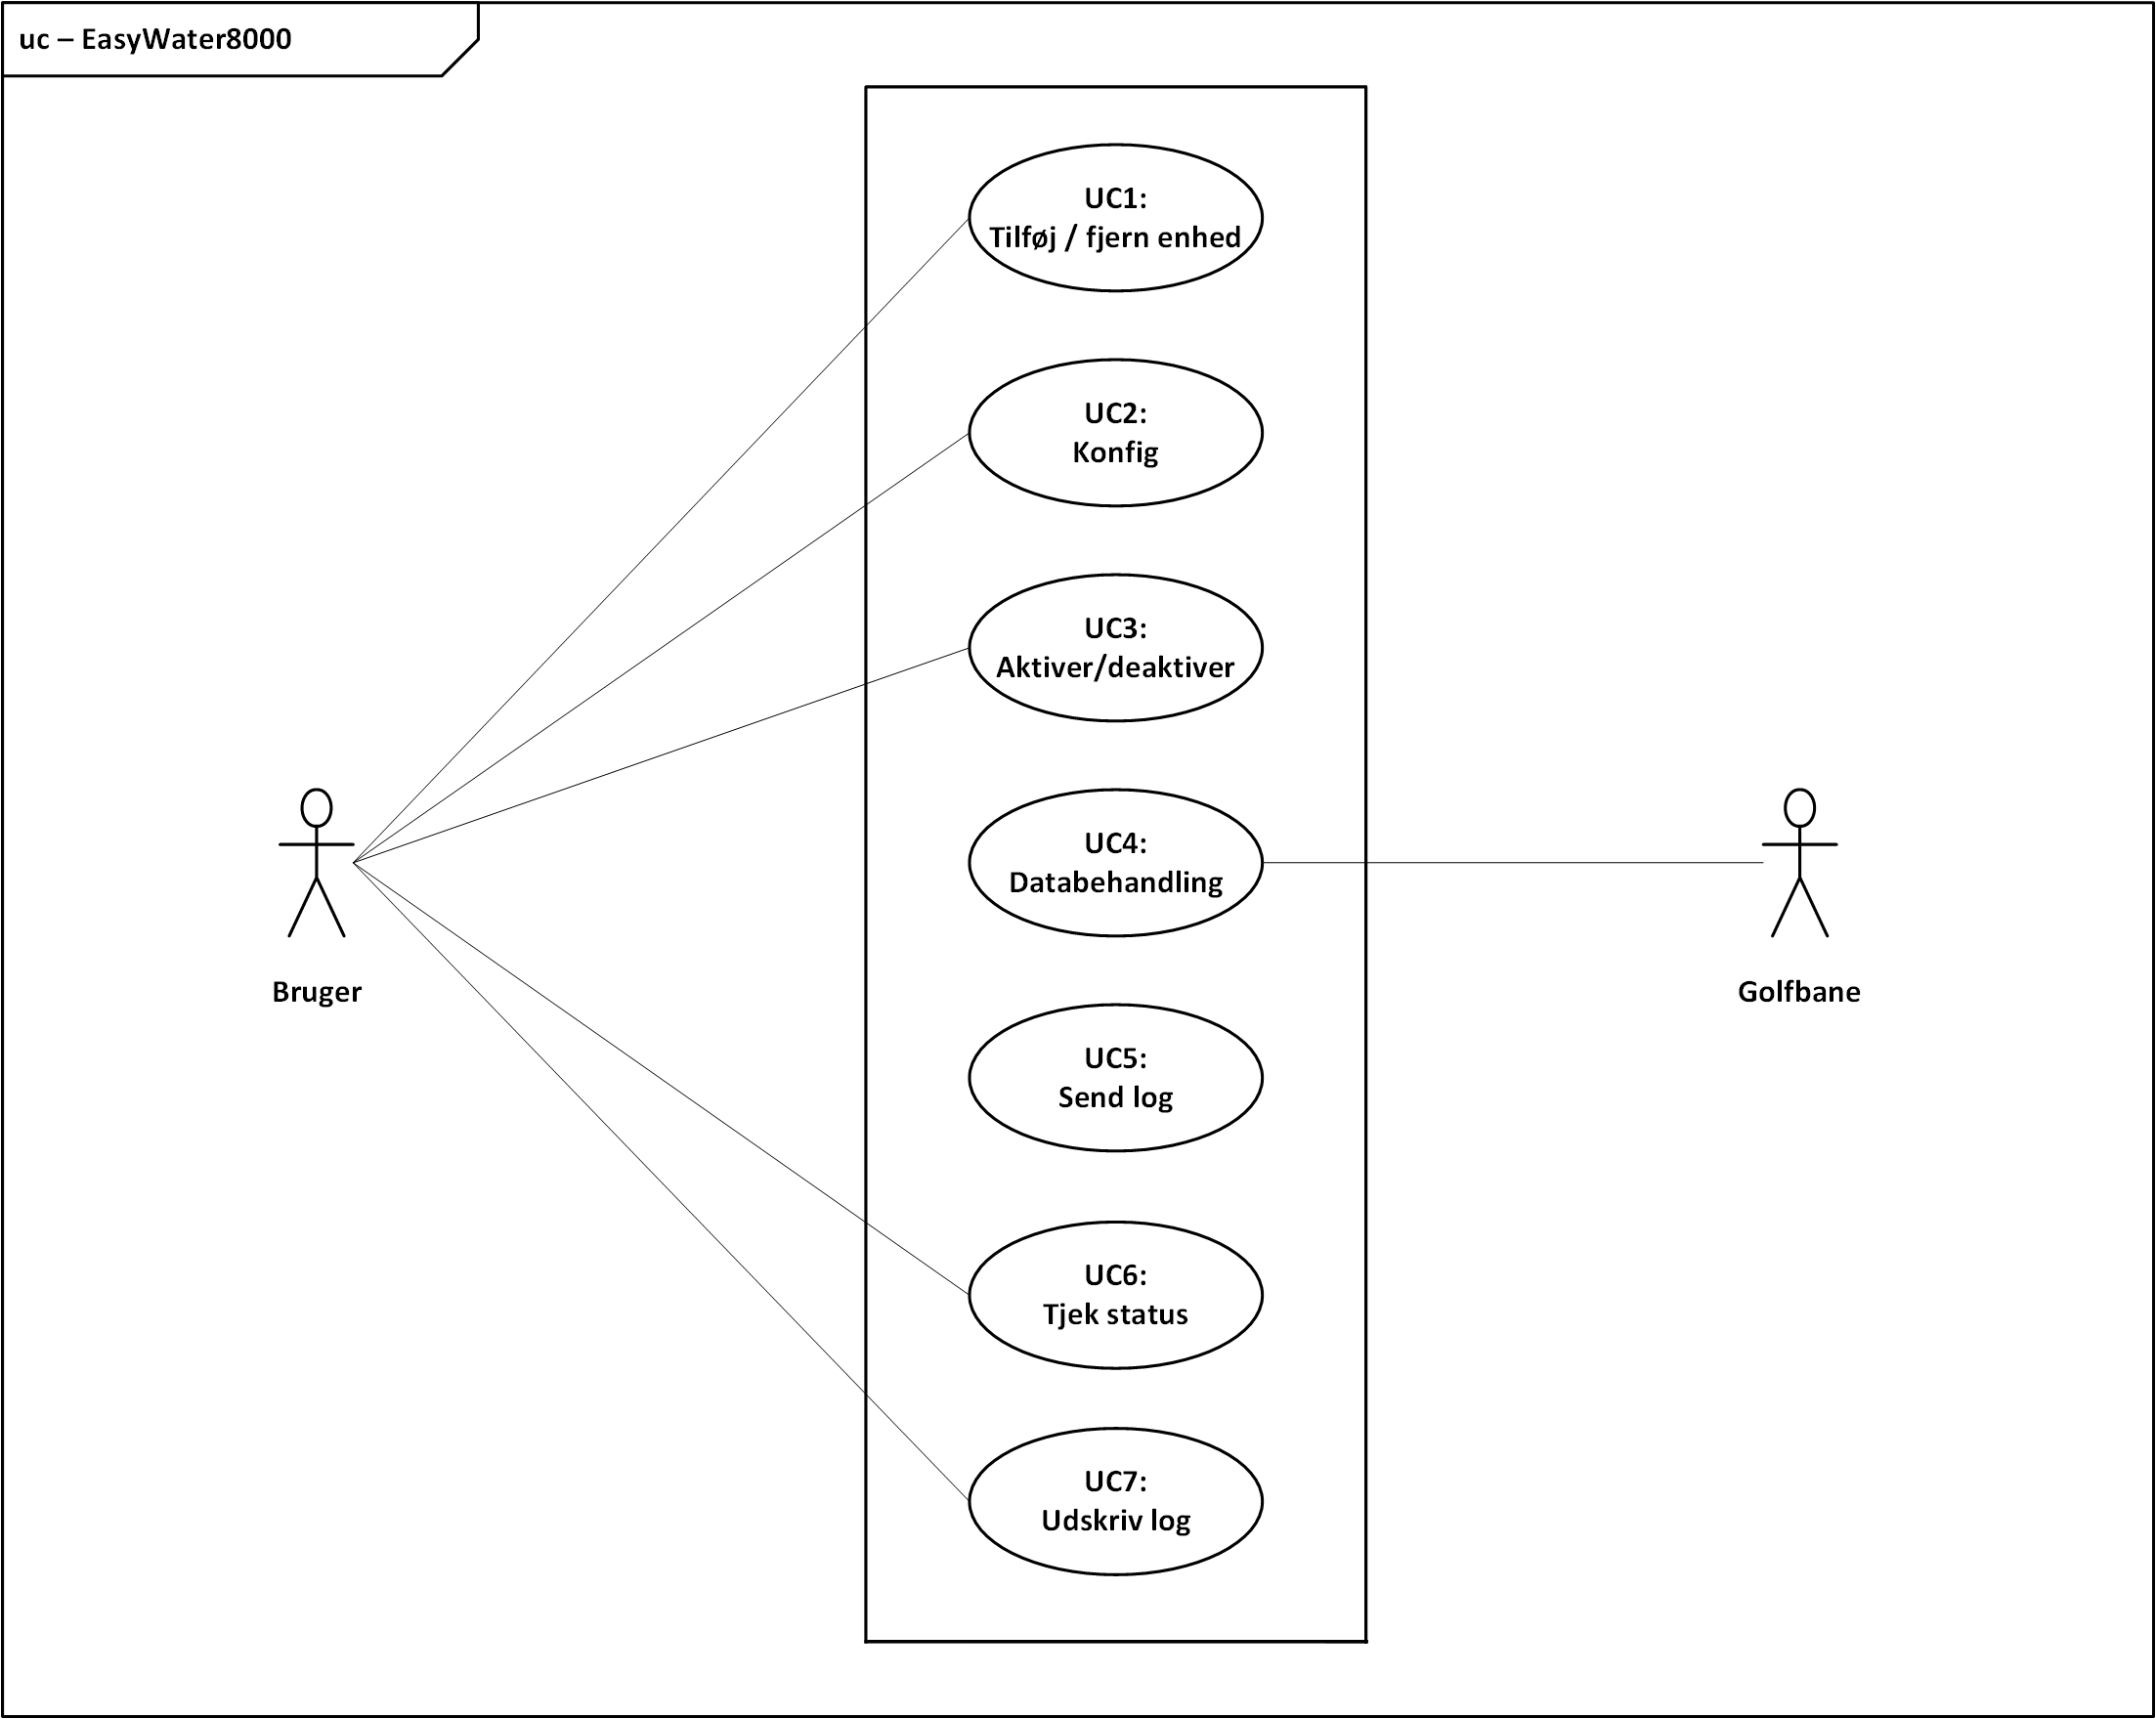
\includegraphics[width=\textwidth]{filer/kravspec/visio/Usecase_Diagram}
\caption{Usecase diagram}
\label{lab:usecasediagram}
\vspace*{\fill}
\end{figure}


\newpage
% UC1: Tilføj/fjern enhed

\subsection{UC1: Tilføj/fjern enhed}
\begin{center} \centering \label{UC1}
	\begin{longtable}{|p{5cm}|p{9cm}|}  %% Longtable = forsætter på næste side
	\hline
		\multicolumn{2}{|l|}{\textbf{UC1: Tilføj\slash fjern enhed}} \\\hline %% HUSK UCECASE NUMMER + NAVN
		\endfirsthead
		
		\multicolumn{2}{l}{...fortsat fra forrige side} \\ \hline %% Til LONGTABLE
		\multicolumn{2}{|l|}{\textbf{UC1: Tilføj\slash fjern enhed}} \\\hline %% HUSK UCECASE NUMMER + NAVN
		\endhead	
		
		\textbf{Mål}								&Bruger kan tilføje eller fjerne Enheder fra systemet			\\\hline
		\textbf{Initialisering}					&Bruger														\\\hline
		\textbf{Aktører og Stakeholders}			&Bruger(Primær)												\\\hline 
		\textbf{Referencer}						&Ingen														\\\hline
		\textbf{AASH}							&1															\\\hline
		\textbf{Efterfølgende tilstand}			&Ønsket Enhed er tilføjet eller fjernet fra systemet		\\\hline
		\textbf{Hovedforløb}					
			&\begin{enumerate}
	
				\item Bruger vælger ''Tilføj eller fjern enhed'' i hovedmenuen
				
				\item En liste af opsatte enheder præsenteres på skærmen				
				
				\item \label{uc1valg} Bruger vælger ''Tilføj''
				
				\begin{enumerate}
					\item \label{uc1indtast} Master beder bruger om at indtaste informationer
					
					\item \label{uc1indtast_fejl} Bruger indtaster hul-nr., adresse og parametre på Enhed
										
					\item Enhed forbindes til kommunikationsnetværket
					
					\item \label{uc1verif} Master verificerer forbindelsen til Enhed
						
					\textbf{[Undtagelse \ref{uc1verif}.a]} \newline
					Enheden kan ikke verificeres
					
					\item Master tilføjer Enhed til systemet

				\end{enumerate}

				\item Bruger vælger celle og trykker ''Fjern''

				\begin{enumerate}

					\item Master deaktiverer Enhed
					
					\item Master sletter Enhed fra systemet
				
				\end{enumerate}
				
				\item Master opdaterer liste med opsatte enheder
				
				\item Bruger kan returnere til hovedmenuen eller opsætte ny enhed (Gå til UC1.\ref{uc1valg})
			\end{enumerate}\\\hline
		\textbf{Undtagelser}
			&\begin{enumerate}[label=\ref{uc1verif}.a]
				
				\item Master viser fejlbesked angående verificering af enheden. Bruger kan forsøge igen (Gå til UC1.\ref{uc1verif} eller vælge ''Tilbage'')

			\end{enumerate}														\\\hline
	\end{longtable} 
\end{center}

%% TIPS:
%% LABEL TIL PUNKT: \label{labelnavn}
%% REFERENCE: \ref{labelnavn}

% UC2: Konfig

\subsection{UC2: Konfig}
\begin{center} \centering
	\begin{longtable}{|p{6cm}|p{8cm}|}  %% Longtable = forsætter på næste side
	\hline
		\multicolumn{2}{|l|}{\textbf{UC2: Aktiver/deaktiver}} \\\hline %% HUSK UCECASE NUMMER + NAVN
		\endfirsthead
		
		\multicolumn{2}{l}{...fortsat fra forrige side} \\ \hline %% Til LONGTABLE
		\multicolumn{2}{|l|}{\textbf{UC2: Aktiver/deaktiver}} \\\hline %% HUSK UCECASE NUMMER + NAVN
		\endhead	
		
		\textbf{Mål}								&At bruger kan aktivere og/eller deaktivere enheder			\\\hline
		\textbf{Initialisering}					&Bruger			\\\hline
		\textbf{Aktører og Stakeholders}			&Bruger(primær), PsoC(sekundær), devkit8000(sekundær)			\\\hline
		\textbf{Referencer}						&Ingen			\\\hline
		\textbf{Antal af samtidige hændelser}	&1			\\\hline
		\textbf{Forudsætning}					&devkit8000 er opsat og systemet er idel. Seriel bus er intakt.			\\\hline
		\textbf{Efterfølgende tilstand}			&Ingen			\\\hline
		\textbf{Hovedforløb}					
			&\begin{enumerate}
	
				\item Bruger logger ind på devkit8000
				
				\item Bruger vælger aktiver/deaktiver i hovedmenuen
				
				\item Bruger vælger aktiver eller deaktiver efter ønske
				
				\item Bruger indtaste adresse på valgte enhed for at aktivere eller deaktivere denne
	
			\end{enumerate}\\\hline
	\end{longtable}
	\label{UC2} 
\end{center}

%% TIPS:
%% LABEL TIL PUNKT: \label{labelnavn}
%% REFERENCE: \ref{labelnavn}

% UC3: Aktiver/deaktiver

\subsection{UC3: Aktiver/deaktiver}
\begin{center} \centering \label{UC3} 
	\begin{longtable}{|p{5cm}|p{9cm}|}  %% Longtable = forsætter på næste side
	\hline
		\multicolumn{2}{|l|}{\textbf{UC3: Aktiver/deaktiver}} \\\hline %% HUSK USECASENUMMER + NAVN
		\endfirsthead
		
		\multicolumn{2}{l}{...fortsat fra forrige side} \\ \hline %% Til LONGTABLE
		\multicolumn{2}{|l|}{\textbf{UC3: Aktiver/deaktiver}} \\\hline %% HUSK USECASENUMMER + NAVN
		\endhead	
		
		\textbf{Mål}								&At aktivere / deaktivere Enhed	\\\hline
		\textbf{Initialisering}					&Bruger				\\\hline
		\textbf{Aktører og Stakeholders}			&Bruger(Primær)		\\\hline
		\textbf{Referencer}						&Ingen				\\\hline
		\textbf{AASH}							&1					\\\hline
		\textbf{Forudsætning}					&Master er opsat og systemet kører \newline
												 Forbindelsen er intakt	\\\hline
		\textbf{Efterfølgende tilstand}			&Enhedstilstand ændres aktiv/deaktiv\\\hline
		\textbf{Hovedforløb}					
			&\begin{enumerate}
	
	
				\item Bruger vælger ''aktiver/deaktiver'' i hovedmenu
				
				\item Bruger markerer enhed ud fra liste af opsatte enheder
				
				\item \label{uc3aktiver} Bruger vælger ''Aktiver'' eller ''Deaktiver'' for at ændre enheden\newline
				\textbf{[Undtagelse \ref{uc3aktiver}.a]} Bruger vælger ''Afbryd''
				
				\item Master udskriver på dennes skærm, at ønsket Enhed er aktiveret eller deaktiveret		
			
				\item Bruger vælger ''Afslut''
				
				\item Master viser hovedmenu	
	
			\end{enumerate}\\\hline
			
		\textbf{Undtagelser}
			&\begin{enumerate}[label=\ref{uc3aktiver}.a]
				
				\item Bruger vælger ''Afbryd''
				
					\subitem Master viser hovedmenu
			\end{enumerate}\\\hline			
			
	\end{longtable}
\end{center}

%% TIPS:
%% LABEL TIL PUNKT: \label{labelnavn}
%% REFERENCE: \ref{labelnavn}

% UC4: Indsamle data

\subsection{UC4: Databehandling}
\begin{center} \centering \label{UC4}
	\begin{longtable}{|p{5cm}|p{9cm}|}  %% Longtable = forsætter på næste side
	\hline
		\multicolumn{2}{|l|}{\textbf{UC4: Indsamle data}} \\\hline %% HUSK USECASENUMMER + NAVN
		\endfirsthead
		
		\multicolumn{2}{l}{...fortsat fra forrige side} \\ \hline %% Til LONGTABLE
		\multicolumn{2}{|l|}{\textbf{UC4: Indsamle data}} \\\hline %% HUSK USECASENUMMER + NAVN
		\endhead	
		
		\textbf{Mål}								&Indsamle data fra omkringliggende jord. Temperatur, fugt og bevægelse			\\\hline
		\textbf{Initialisering}					&Enhedstimer			\\\hline
		\textbf{Aktører og Stakeholders}			&Omgivelser				\\\hline
		\textbf{Referencer}						&UC8: Vanding		\\\hline
		\textbf{AASH}							&1 per Enhed			\\\hline
		\textbf{Forudsætning}					&Aktiv Enhed			\\\hline
		\textbf{Efterfølgende tilstand}			&Data gemt i Enhed 	\\\hline
		\textbf{Hovedforløb}					
			&\begin{enumerate}
	
				\item Sensorer måler kontinuert temperatur og fugt i banen og bevægelse på banen
				
				\item Enhed henter temperatur- og fugtdata samt vandingsstatus ved hver udløb af Enhedstimer
				
				\item Enhed gemmer data				
				
				\item Enhed modtager data ved bevægelse  
				
			\end{enumerate}\\\hline
	\end{longtable}
\end{center}

%% TIPS:
%% LABEL TIL PUNKT: \label{labelnavn}
%% REFERENCE: \ref{labelnavn}

% UC5: Tjek status

\subsection{UC5: Tjek status}
\begin{center} \centering \label{UC5} 
	\begin{longtable}{|p{5cm}|p{9cm}|}  %% Longtable = forsætter på næste side
	\hline
		\multicolumn{2}{|l|}{\textbf{UC5: Vanding}} 		\\\hline %% HUSK UCECASE NUMMER + NAVN
		\endfirsthead
		
		\multicolumn{2}{l}{...fortsat fra forrige side} 	\\ \hline %% Til LONGTABLE
		\multicolumn{2}{|l|}{\textbf{UC5: Vanding}} 		\\\hline %% HUSK UCECASE NUMMER + NAVN
		\endhead	
		
		\textbf{Mål}								&At vande trængende områder	\\\hline
		\textbf{Initialisering}					&Ingen						\\\hline
		\textbf{Aktører og Stakeholders}			&Golfbane(Primær)			\\\hline
		\textbf{Referencer}						&UC4: Indsamle data 			\\\hline
		\textbf{AASH}							&1							\\\hline
		\textbf{Forudsætning}					&Aktiv Enhed					\\\hline
		\textbf{Efterfølgende tilstand}			&Aktiv						\\\hline
		\textbf{Hovedforløb}					
			&\begin{enumerate}
				
				\item Enhed læser fugt- og temperaturværdier fra UC4: Indsamle data
				
				\item \label{uc5sprinkler} Vanding startes på områder med for lave værdier
				
					\textbf{[Undtagelse \ref{uc5sprinkler}a]} Bevægelse registreret
	
			\end{enumerate}\\\hline

		\textbf{Undtagelser}
			&\begin{enumerate}[label=\ref{uc5sprinkler}a.]
			
				\item Sprinkler deaktiveres i 30 minutter og herefter gentages hovedforløb	
			
			\end{enumerate}\\\hline
	\end{longtable}
\end{center}

%% TIPS:
%% LABEL TIL PUNKT: \label{labelnavn}
%% REFERENCE: \ref{labelnavn}

% UC6: Udskriv log

\subsection{UC6: Udskriv log}
\begin{center} \centering
	\begin{longtable}{|p{6cm}|p{8cm}|}  %% Longtable = forsætter på næste side
	\hline
		\multicolumn{2}{|l|}{\textbf{UC1: USECASENAVN}} \\\hline %% HUSK UCECASE NUMMER + NAVN
		\endfirsthead
		
		\multicolumn{2}{l}{...fortsat fra forrige side} \\ \hline %% Til LONGTABLE
		\multicolumn{2}{|l|}{\textbf{UC1: USECASENAVN}} \\\hline %% HUSK UCECASE NUMMER + NAVN
		\endhead	
		
		\textbf{Mål}								&Skriv her			\\\hline
		\textbf{Initialisering}					&Skriv her			\\\hline
		\textbf{Aktører og Stakeholders}			&Skriv her			\\\hline
		\textbf{Referencer}						&Skriv her			\\\hline
		\textbf{Antal af samtidige hændelser}	&Skriv her			\\\hline
		\textbf{Forudsætning}					&Skriv her			\\\hline
		\textbf{Efterfølgende tilstand}			&Skriv her			\\\hline
		\textbf{Hovedforløb}					
			&\begin{enumerate}
	
				\item %%Punkt 1
				
				\item %%Punkt 2
				
				\item %%Etc.
	
			\end{enumerate}\\\hline
	\end{longtable}
	\label{UC6} 
\end{center}

%% TIPS:
%% LABEL TIL PUNKT: \label{labelnavn}
%% REFERENCE: \ref{labelnavn}

%% Ikke-funktionelle krav

\section{Ikke-funktionelle krav}\label{header:ikke-funk}
% Ikke-funktionelle krav
\begin{enumerate}

\subsubsection*{Brugbarhed}
\item Opsætningen skal ske af autoriseret personale
\item UI skal kunne benyttes af bruger efter gennemlæst manual


\subsubsection*{Pålidelighed}
\item Levetid: 2 år uden hardware nedbrud
\item Software IDLE tid: minimum 1 måned uden restart


\subsubsection*{Ydeevne}
\item Master skal kunne håndtere minimum 18 enheder
\item Sprinkler skal kunne vande et areal afdækket af 360 grader med radius min. 3.5 m 
\item Der skal kunne tilføjes yderligere enheder efter opsætning af systemet


\subsubsection*{Vedligeholdelse}
\item Enheder skal være udskiftelige uden at det er nødvendigt at tilgå sensorer eller sprinkler
\item Sprinklere skal være let tilgængelige for personale


\subsubsection*{Generelle krav}
\item Al kommunikation sker via en seriel bus 


\subsubsection*{Enheder}
\item Enhed skal kunne operere autonomt efter denne er sat op fra Master
\item Enheder skal sende log information til Master efter hver udførte måling
\item Enheder skal sende log information til Master efter hver udført vanding

\end{enumerate}

\subsubsection*{Begrænsninger}
\begin{itemize}
\item Der udarbejdes en skaleret udgave, da vi ikke har adgang til en hel golfbane
\item Grundet tidsbegrænsninger udvikles der ikke et fuldt system 
\item Som minimum skal der produceres funktionel Master og én komplet Enhed
\item Systemet udvikles således, at der til hver sprinkler tilhører en pumpe. Denne løsning vil ikke vælges i en produktionsudgave, her vil der være én vandforsyning, med et tryk stort nok, til at tilføre samtlige sprinklere, den nødvendige mængde vand. Sprinklerne vil i denne færdige udgave styres vha. magnetventiler 
% Skal uddybes i fremtidigt atbejde ?
\end{itemize}





\section{Grafiske brugerflade-skitser (BS)}
\label{subsec:GUI}
%% SW arkitektur: GUI skitser

Inden det endelige GUI udvikles laves nogle skitser som udviklingen læner sig op af. Ud fra UC beskrivelserne findes de skærmbilleder som skal vises på Master og skitseres.

Her følger korte beskrivelser af hver skitse samt skitsen selv.

\subsubsection{Startmenu}
Figur \ref{fig:GUI-Startmenu} er den første menu brugeren kommer til. Her er valgmulighederne præsenteret for brugeren.

\begin{figure}[htbp] \centering
{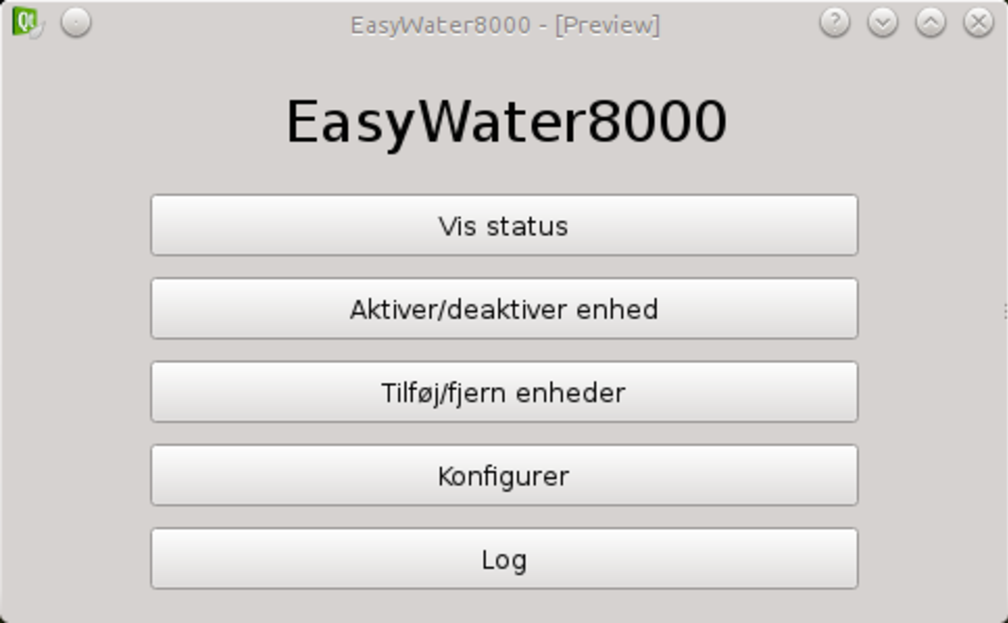
\includegraphics[scale=0.5]{filer/pics/GUI/Start-menu}}
\caption{Skitse af startmenu på GUI}
\label{fig:GUI-Startmenu}
\end{figure}

\subsubsection{Vis Status}
På figur \ref{fig:GUI-aktuel-status} vises den aktuelle status af systemets enheder. Den øverste række tal er tilkoblede Enheder. Den anden række tal er komponentpakker tilkoblet den enkelte enhed.

\begin{figure}[htbp] \centering
{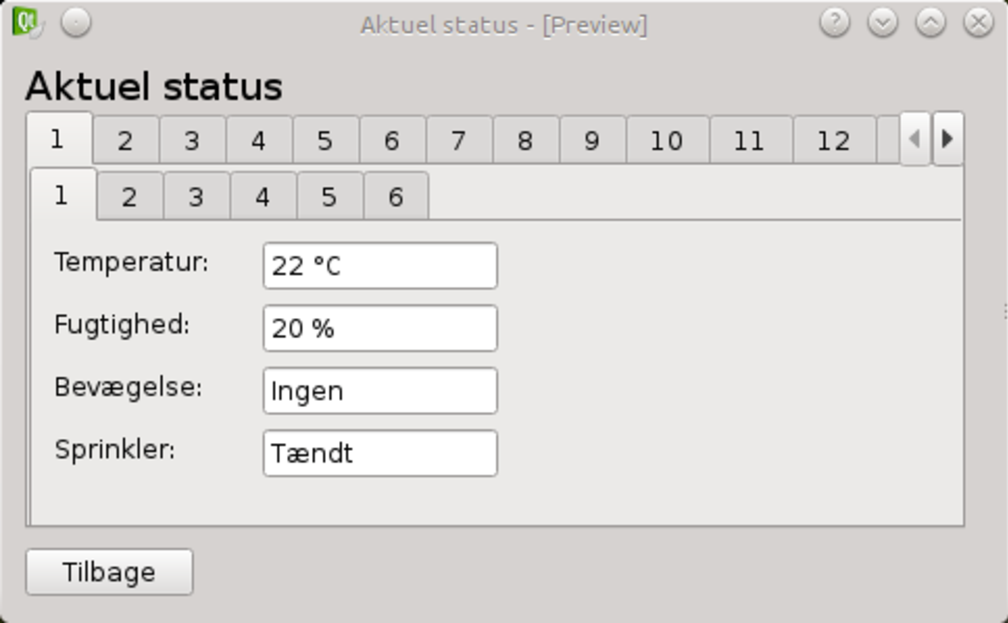
\includegraphics[scale=0.5]{filer/pics/GUI/Aktuel-status}}
\caption{Skitse af ''Vis status'' på GUI}
\label{fig:GUI-aktuel-status}
\end{figure}

\subsubsection{Aktiver og deaktiver enhed}
Skitsen på figur \ref{fig:GUI-aktiver-deaktiver} viser brugerens mulighed for at aktivere og deaktivere enkelte enheder i systemet.

\begin{figure}[htbp] \centering
{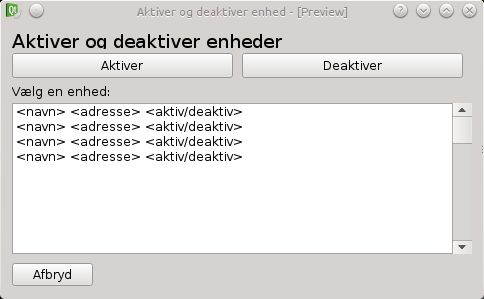
\includegraphics[scale=0.5]{filer/pics/GUI/Aktiver-deaktiver-enheder}}
\caption{Skitse af ''Aktiver og deaktiver enhed'' på GUI}
\label{fig:GUI-aktiver-deaktiver}
\end{figure}

\subsubsection{Tilføj/fjern enheder}
De præsenterede muligheder i forbindelse med at fjerne og tilføje enheder til systemet er vist på figur \ref{fig:GUI-tilfoj-fjern}.

\begin{figure}[htbp] \centering
{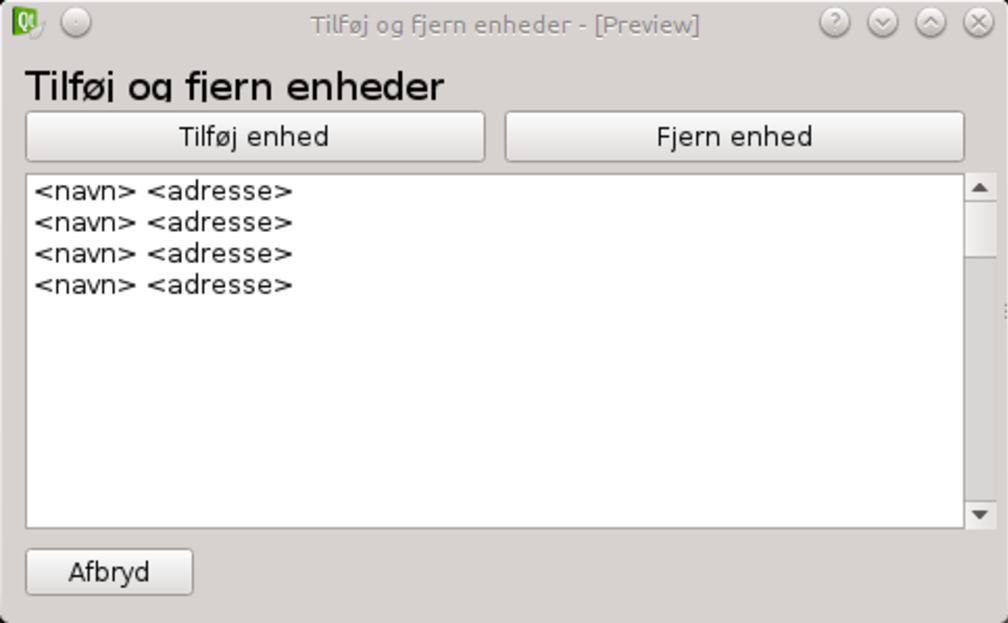
\includegraphics[scale=0.5]{filer/pics/GUI/Tilfoj-fjern-enheder}}
\caption{Skitse af ''Tilføj/fjern enheder'' på GUI}
\label{fig:GUI-tilfoj-fjern}
\end{figure}

\subsubsection{Konfigurer}
Når brugeren skal konfigurerer en enhed bruges skitsen på figur \ref{fig:GUI-konfigurer}. Her vælger brugeren hvilken enhed der skal konfigureres.

\begin{figure}[htbp] \centering
{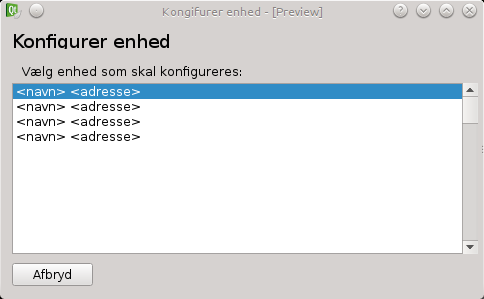
\includegraphics[scale=0.5]{filer/pics/GUI/Konfigurer-enhed}}
\caption{Skitse af ''Konfigurer'' på GUI}
\label{fig:GUI-konfigurer}
\end{figure}

\subsubsection{Indstil parametre}
Når brugeren har valgt en enhed som skal konfigureres vises skærmen på figur \ref{fig:GUI-indstil-parametre}. Her kan brugeren indtaste parametrene for enheden.

\begin{figure}[htbp] \centering
{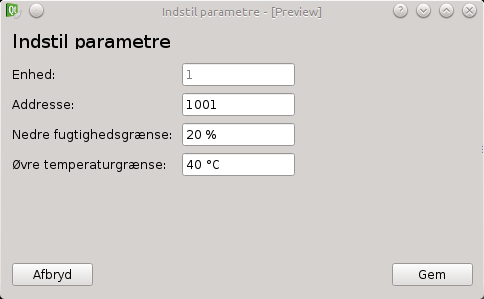
\includegraphics[scale=0.5]{filer/pics/GUI/Indstil-parametre}}
\caption{Skitse af ''Indstil parametre'' på GUI}
\label{fig:GUI-indstil-parametre}
\end{figure}

\subsubsection{Log}
Loggen præsenterer de indsamlede data fra alle enhederne. Det er muligt at se alle data på en gang, som vist på figur \ref{fig:GUI-log-alle}, hvor den øverste fanerække er numre på opsatte enheder i systemet, eller man kan vælge de enkelte enheder og se deres forskellige komponentpakker, som vist på figur \ref{fig:GUI-log-enhed}, hvor den anden fanerække er komponentpakker koblet op på systemet.

\begin{figure}[htbp] \centering
{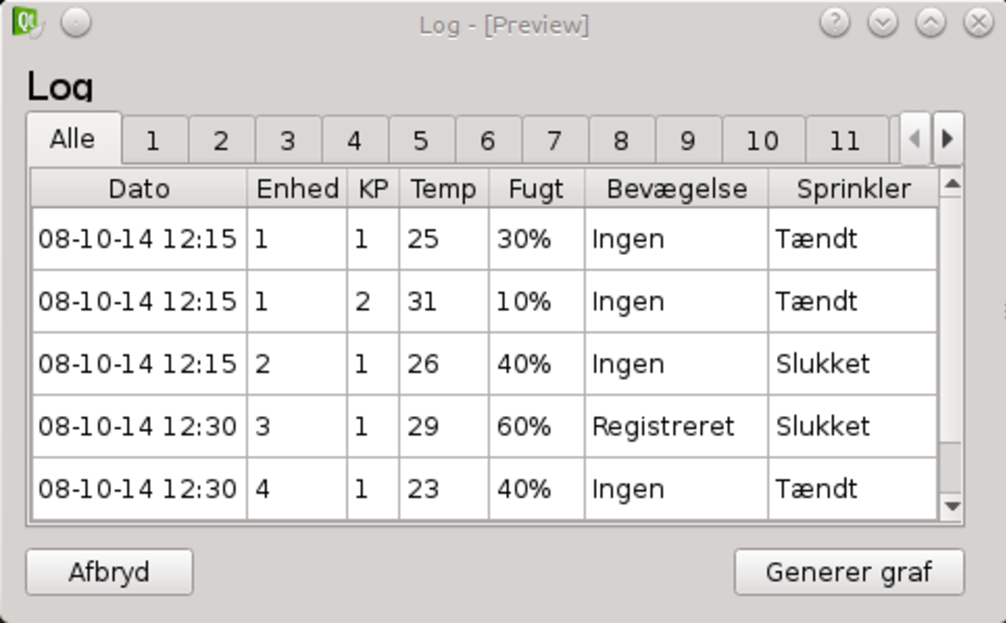
\includegraphics[scale=0.5]{filer/pics/GUI/Log-alle}}
\caption{Skitse af ''Log'' for alle enheder på GUI}
\label{fig:GUI-log-alle}
\end{figure}

\begin{figure}[htbp] \centering
{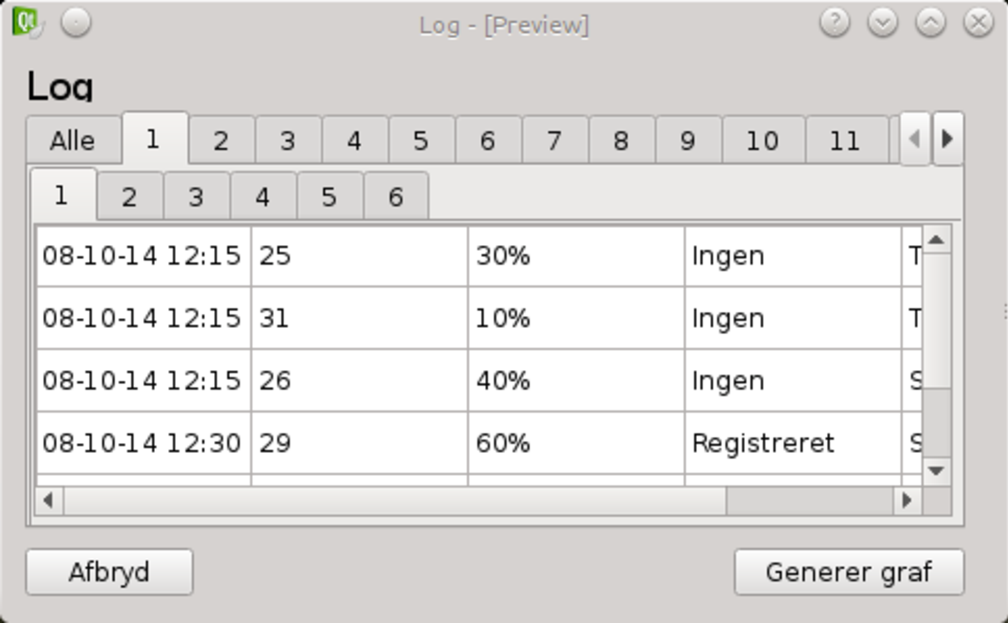
\includegraphics[scale=0.5]{filer/pics/GUI/Log-enhed}}
\caption{Skitse af ''Log'' for enkelt enhed på GUI}
\label{fig:GUI-log-enhed}
\end{figure}





% Arbejdsprocessen


\chapter{Arbejdsproces}

\section{Udviklingsmodeller}
Gruppearbejdet til dette semester-projekt har taget udgangspunkt i arbejdsmetoden fra sidste semester, i det gruppen dengang havde succes med netop denne. Arbejdsmetoden tager udgangspunkt i ASE-modellen, se figur \ref{fig:ASE_modellen}. ASE-modellen har en fælles fase og en fagspecifik fase. Gruppen har arbejdet sammen i fællesfasen med udarbejdelse af projektformulering, kravspecifikation, accepttest og til dels systemarkitektur. Herefter har gruppen arbejdet i teams i den fagspecifikke fase, hvor design og implementeringen ligger. Efter den fagspecifikke fase samles gruppen igen i en fælles fase for den endelige accepttest udføres og rapport udarbejdes. 

%ASE MODELLEN BILLEDE
\begin{figure}[h]
  \centering
    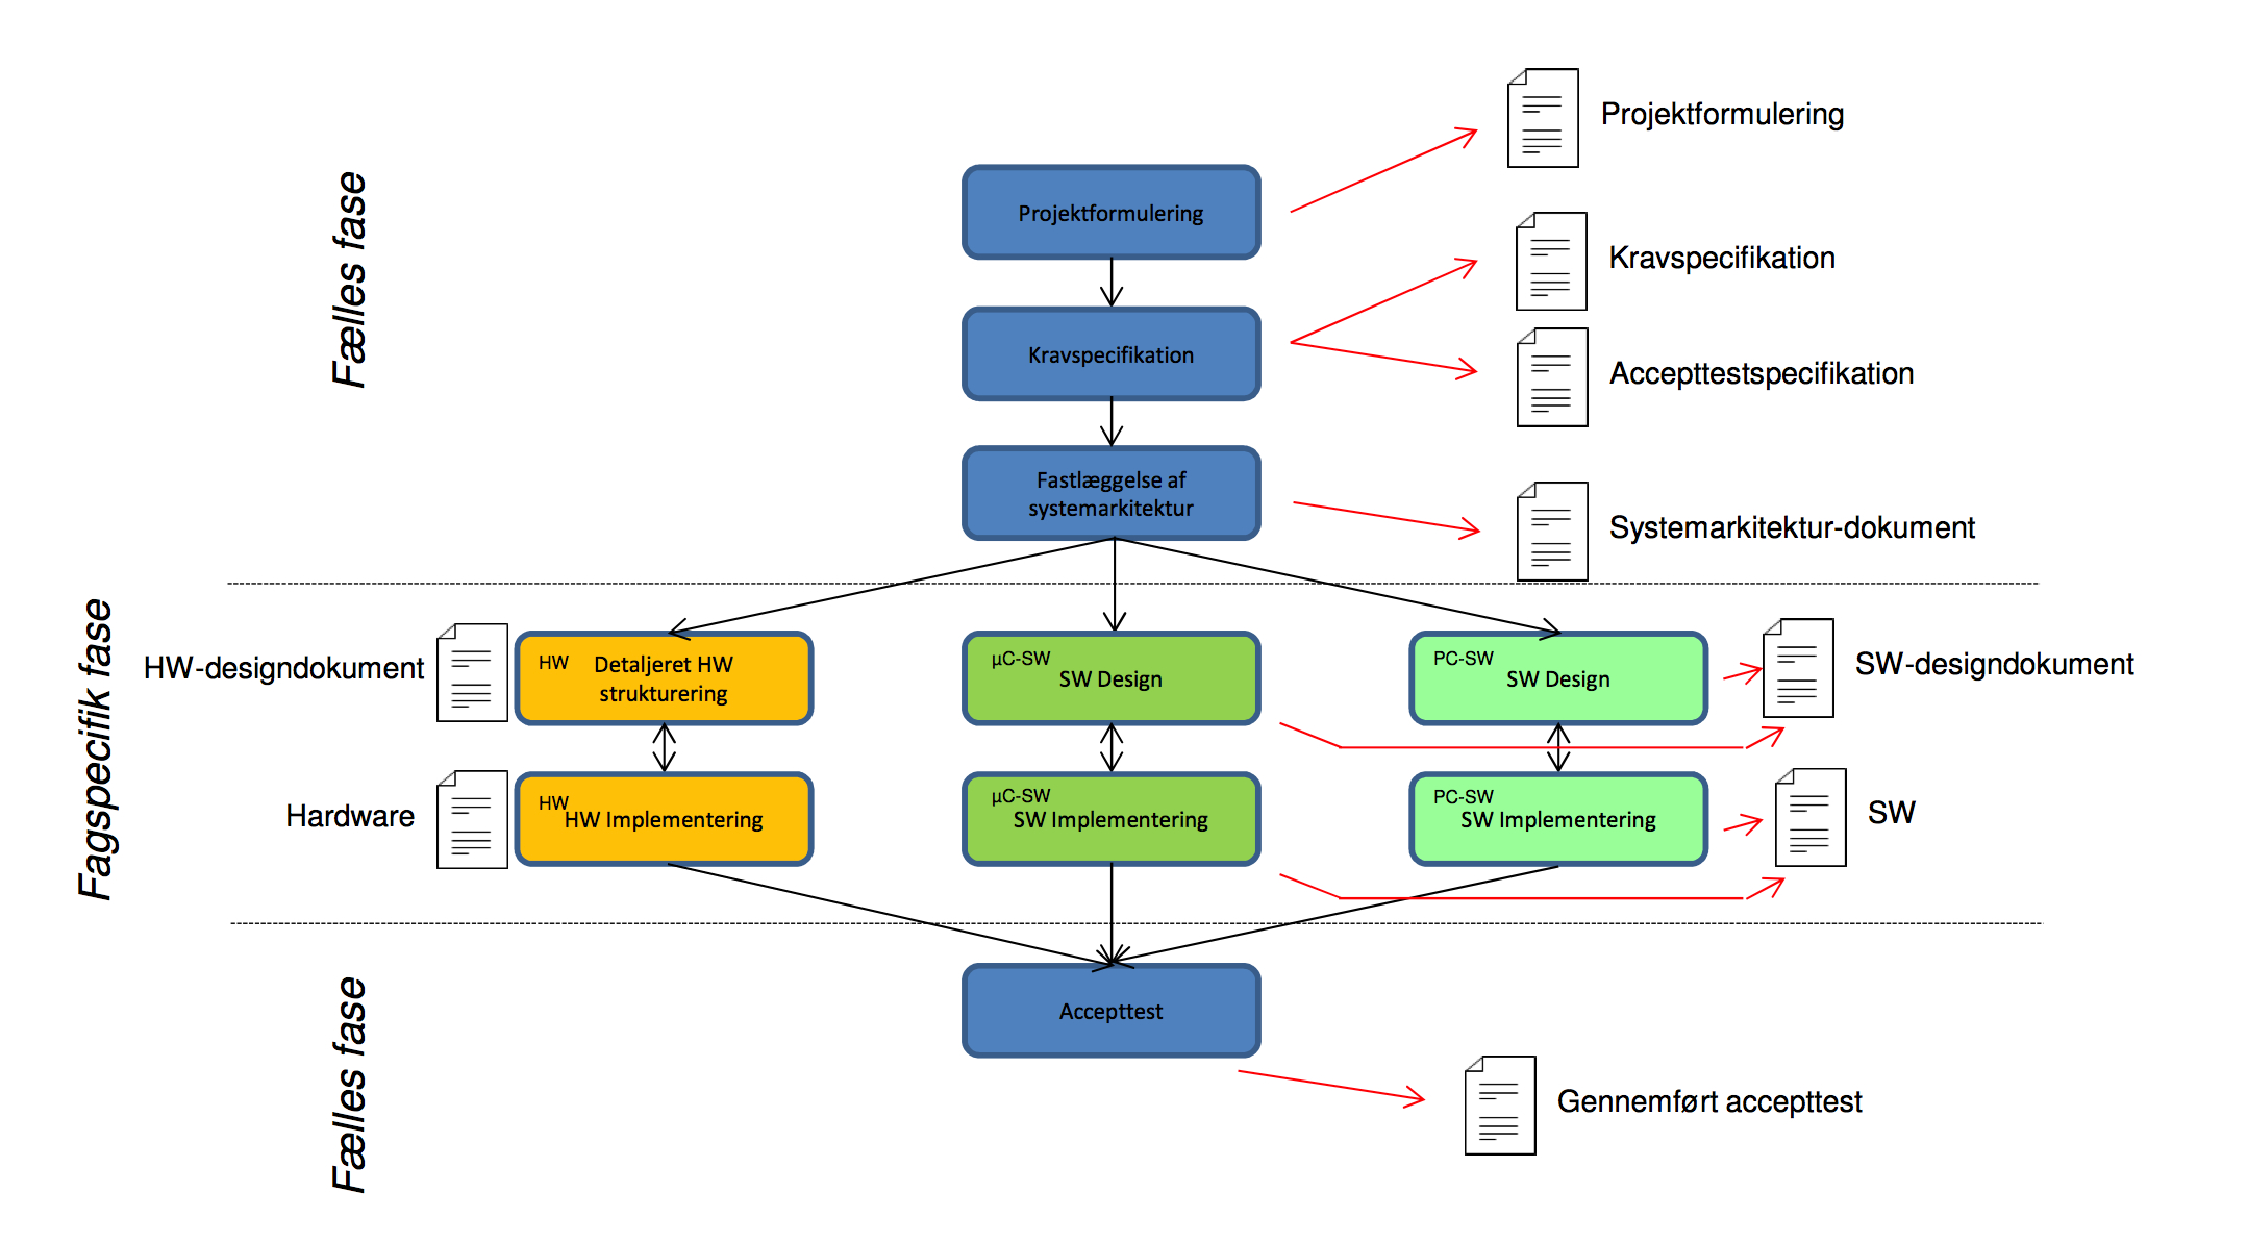
\includegraphics[width=\textwidth]{Billeder/ASE_modellen}
    \caption{ASE-modellen}
    \label{fig:ASE_modellen}
\end{figure}

V-modellen, se figur \ref{fig:V_modellen}, er benyttet sammen med ASE-modellen. V-modellen bygger på at hver enkelt delfase afsluttes før en ny delfase påbegyndes. En test af hver fase planlægges ved slutningen af den forgående. 

%V-MODELLEN BILLEDE
\begin{figure}[h]
  \centering
    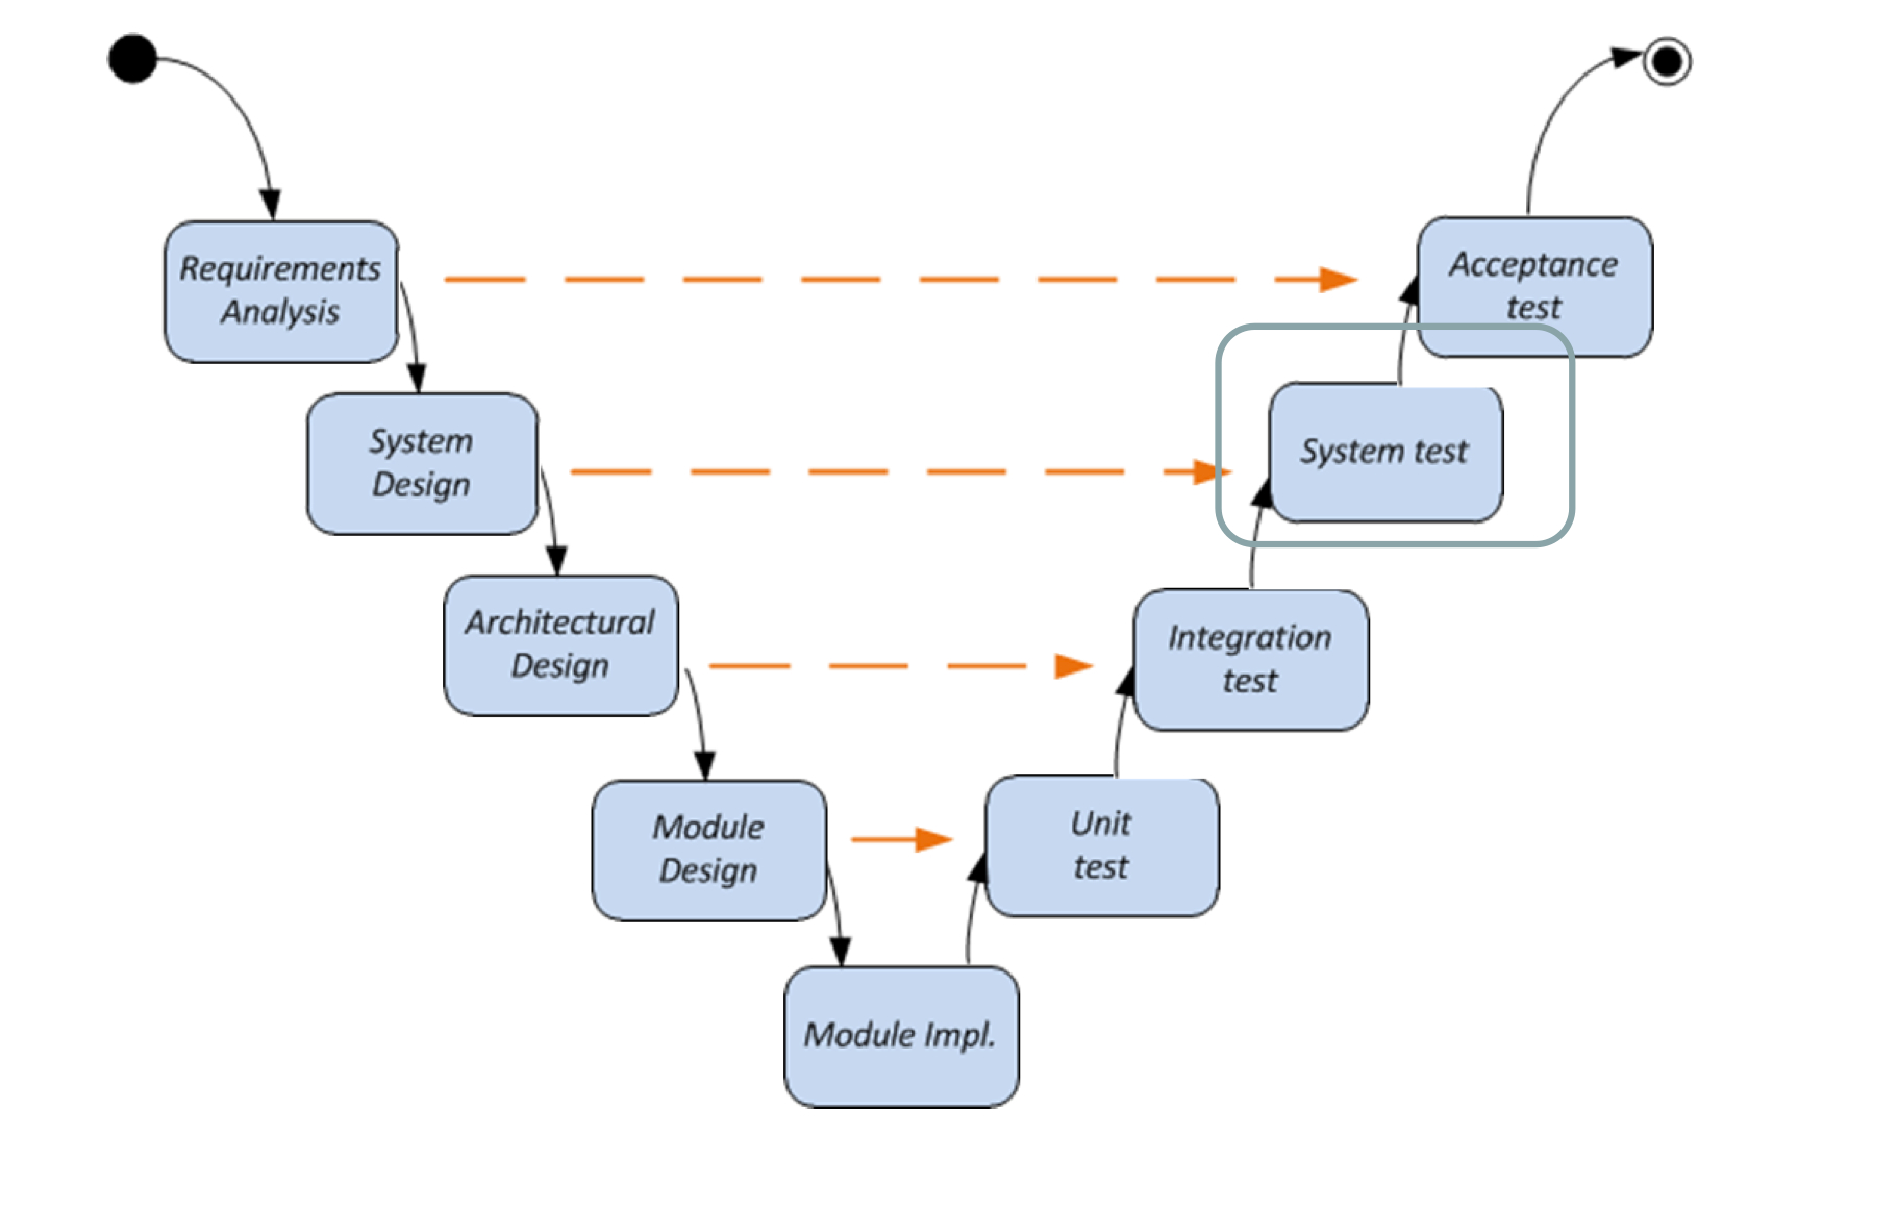
\includegraphics[width=\textwidth]{Billeder/V_modellen}
    \caption{V-modellen}
    \label{fig:V_modellen}
\end{figure}

\section{Møder, tidsplan, logbog og referater}

I forbindelse med gennemførelse af dette projekt er der afholdt en række møder. Gruppemøder, vejledermøder samt reviewmøder. 

Som hovedregel har der været afholdt ét vejleder møde og mindst ét gruppemøde hver uge, dog med enkelte undtagelser. 

Vejledermødet har været fast hver tirsdag. Dette møde har fungeret som den primære kontakt mellem gruppen og vejleder. Vejleren har ofte haft adgang til foreløbig dokumentation, som vejlederen har givet konstruktiv feedback på.

Gruppemøderne har haft et fast punkt: Status, hvem er i gang med hvad og hvor langt er hver i sær med de pågældende opgaver. Ydermere er der afholdt tre trivselsrunder. Disse giver mulighed for at give ris/ros til de enkelte gruppemedlemmer samt mulighed for at gøre opmærksom på ikke-projekt-relaterede emner. 
Gruppen har fra start udarbejdet en gruppekontrakt\footnote{Gruppekontakten foreligger på bilags-CDen navn: Gruppekontrakt.pdf}. Denne kontrakt udgør et fælles standpunkt for gruppen og de indbyrdes aftaler. Gruppen indførte et koncept kaldet ''Stå-op-møde'', dvs. et møde der tager under 10 minutter. Mødets mål er planlagt, således at tiden ikke spildes. 

Der er afholdt reviews. Et review af kravspecifikationen samt et review af systemarkitekturen. 
Disse reviews har fået afklaret nogle problemstillinger som reviewgruppen fremlagde. 
Gruppen aftalte efter samtale med gruppe 2, at aflyse review af deres systemarkitektur, da de ikke ville vente med at rette dokumentet til før reviewet var modtaget, dette skete med vejleders sammentykke.  

Alle møder er skrifteligt dokumenteret af sekretæren med logbog og mødereferater. 

Tidsplanen\footnote{Tidsplanen forefindes på bilags-CDen. Navn: Tidsplan.pdf} er løbende blevet opdateret 

\section{Arbejdsfordeling}

Gruppen har som helhed haft et godt og solidt samarbejde. 

Allerede en måned efter projekts start oplevede gruppen ustabilitet i Jeppe Stærks fremmøde. Jeppe havde private problemer, som vi i gruppen selvfølgelig mente, at han skulle have tid til. Sidste gang vi så og hørte fra Jeppe var i uge 41. Siden har han, af ukendte årsager, valgt at ignorere alt kontakt til gruppen og dens medlemmer. Gruppen valgte d. 27/10-2014 at meddele Jeppe, skrifteligt, at han fra dags dato var ude af gruppen.     

\subsection{Arbejdsgrupper}
Gruppen har hovedsagligt været opdelt i tre mindre arbejdsgrupper i forbindelse med faserne: Design, implementering og modultest. Forfattere til de enkelte kapitler er angivet med initialer.
Overordnet er opdelingen: HW (Jakob, Lennart, Mick, Poul og Simon) og SW (Bjørn og Jesper). 
HW og SW har arbejdet i nedenstående tre undergrupper.

\textbf{Gruppen indeholdende Bjørn og Jesper} \newline
Bjørn og Jesper har stået for alt software over HW API-niveau. Design og arkitektur er udviklet i tæt samarbejde og selve koden er implementeret ved at uddelegere de forskellige klasser, efterhånden som de er vurderet vigtige og nødvendige.

\textbf{Gruppen indeholdende Jakob og Lennart} \newline
Jakob og Lennart har primært arbejdet med FT-sensoren, både HW- og SW-delen her for. Undervejs i forløbet er arbejdet delt lidt op, så Jakob hovedsageligt arbejdede med softwaren til PSoC4 og Lennart med den fysiske hardware. Der har været et godt arbejde og udregning af filteret samt designet af hele sensoren blev lavet sammen mens implementering heraf blev delt mere op. 


\textbf{Gruppen indeholdende Mick, Poul og Simon} \newline
Mick, Poul og Simon har igennem designfasen arbejdet tæt sammen om SPI-kommunikationen, PIR-sensoren, vandpumpe med tilhørende relæ og tilslutningsprintet. Mick og Poul har herefter stået for implementeringen af SPI-kommunikationen, mens Simon har færdiggjort de andre dele samt implementeret tilslutningsprintet.


\subsection{Rollefordeling}

\textbf{Opsætning \LaTeX dokumenter} \newline
Hovedansvarlig: Mick 

\textbf{Sekretær i forbindelse med logbog og referater} \newline
Hovedansvarlig: Simon

\textbf{Projektleder, mødeindkalder og holder samt tavlestyring } \newline
Hovedansvarlig: Poul

\textbf{Vejlederkontakt} \newline
Hovedansvarlig: Poul   



% Udviklingsværktøjer


\chapter{Udviklingsværktøjer (PO)} \label{head:udviklingsvaektoejer}
I det følgende afsnit beskrives, de benyttede, udviklingsværktøjer i forbindelse med dette projekt. 

\section{LaTeX og TexMaker}
Både denne rapport og tilhørende dokumentation er skrevet i sproget \LaTeX. Største delen af gruppen havde erfaring med \LaTeX fra sidste semester projekt. 

\LaTeX er et tekstbaseret kodesprog som gør brugeren fri af layout således at fokus kan rettes mod indholdet. Det kræver selvfølgelig at man sætter sig ind i dette sprog og overholder kodestandarden. 

TexMaker er benyttet som teksteditor til \LaTeX. Denne editor gør det muligt at navigere rundt imellem forskellige .tex-filer og bygge dokumenterne via TexMakers indbyggede pdf-viewer.

\section{Multisim}
National Instruments Multisim er benyttet til kredsløbsdesign og simulering af disse. 

\section{PSoC Creator}
PSoC Creator fra Cypress er benyttet i forbindelse med softwareprogrammeringen af Enheden (PSoC4). PSoC4 er Cypress' nyeste ARM baserede Programmable System-on-Chip med en Cortex-M0 processor. 

\section{Eclipse}
Eclipse er benyttet i forbindelse med softwareprogrammeringen af Masteren (Devkit8000). Eclipse kræver et Linux baseret operativsystem.

\section{Qt Creator}
Qt Creator er benyttet i forbindelse med den grafiske brugerflade på Masteren (Devkit8000).

\section{Microsoft Visual Studio 13}
Er anvendt til at skrive hardware-uafhængige \verb+C+ klasser til Enheden (PSoC4).

\section{Logic}
Logic fra Salae er en logik analysator der er benyttet til at gemme digitale signaler, så det herefter var muligt at analyse f.eks dele af SPI-kommunikationen. Logic har indbygget SPI-protokol.

\section{EAGLE}
EAGLEs PCB layout editor er benyttet til design af print til FT-sensoren.

\section{Microsoft Visio}
Microsoft Visio er benyttet til at udarbejde UML- og SysML-diagrammer. 

\section{Maple}
Matematik software, til matematiske udregninger og grafer.

\section{Electronic Toolbox}
App af Marcus Roskosch til smartphones og tablets, til at hjælpe med komponent valg på integreret hardware m.m. 

\section{Filhåndtering}
Der er benyttet 2 cloud services i forbindelse med filhåndteringen for dette projekt

\subsection{GitHub}
GitHub er benyttet til versionsstyring af projektdokumenter dvs. Alle .tex-filer til dokumentation og rapport, softwarekildekode, UML- og SysML-diagrammer, Multisim-kredsløbsdiagrammer. GitHub sørger for at alle altid har nyeste version. 

\subsection{Google Drev}
Google Drev er benyttet i flere forskellige forbindelser. Fælles dokumenter, mødereferater, logbog, tidsplan og fælles dokumenter i forbindelse med rette runder.

% Systemarkitektur

\chapter{Systemarkitektur}
Systemarkitekturen består af en række forskellige diagrammer med dertilhørende tekst. Diagrammerne er opbygget efter SysML standarden\footnote{ISE undervisningen på 2. semester}

\begin{figure}[htbp] \centering
\section{Domænemodel (JC)}
{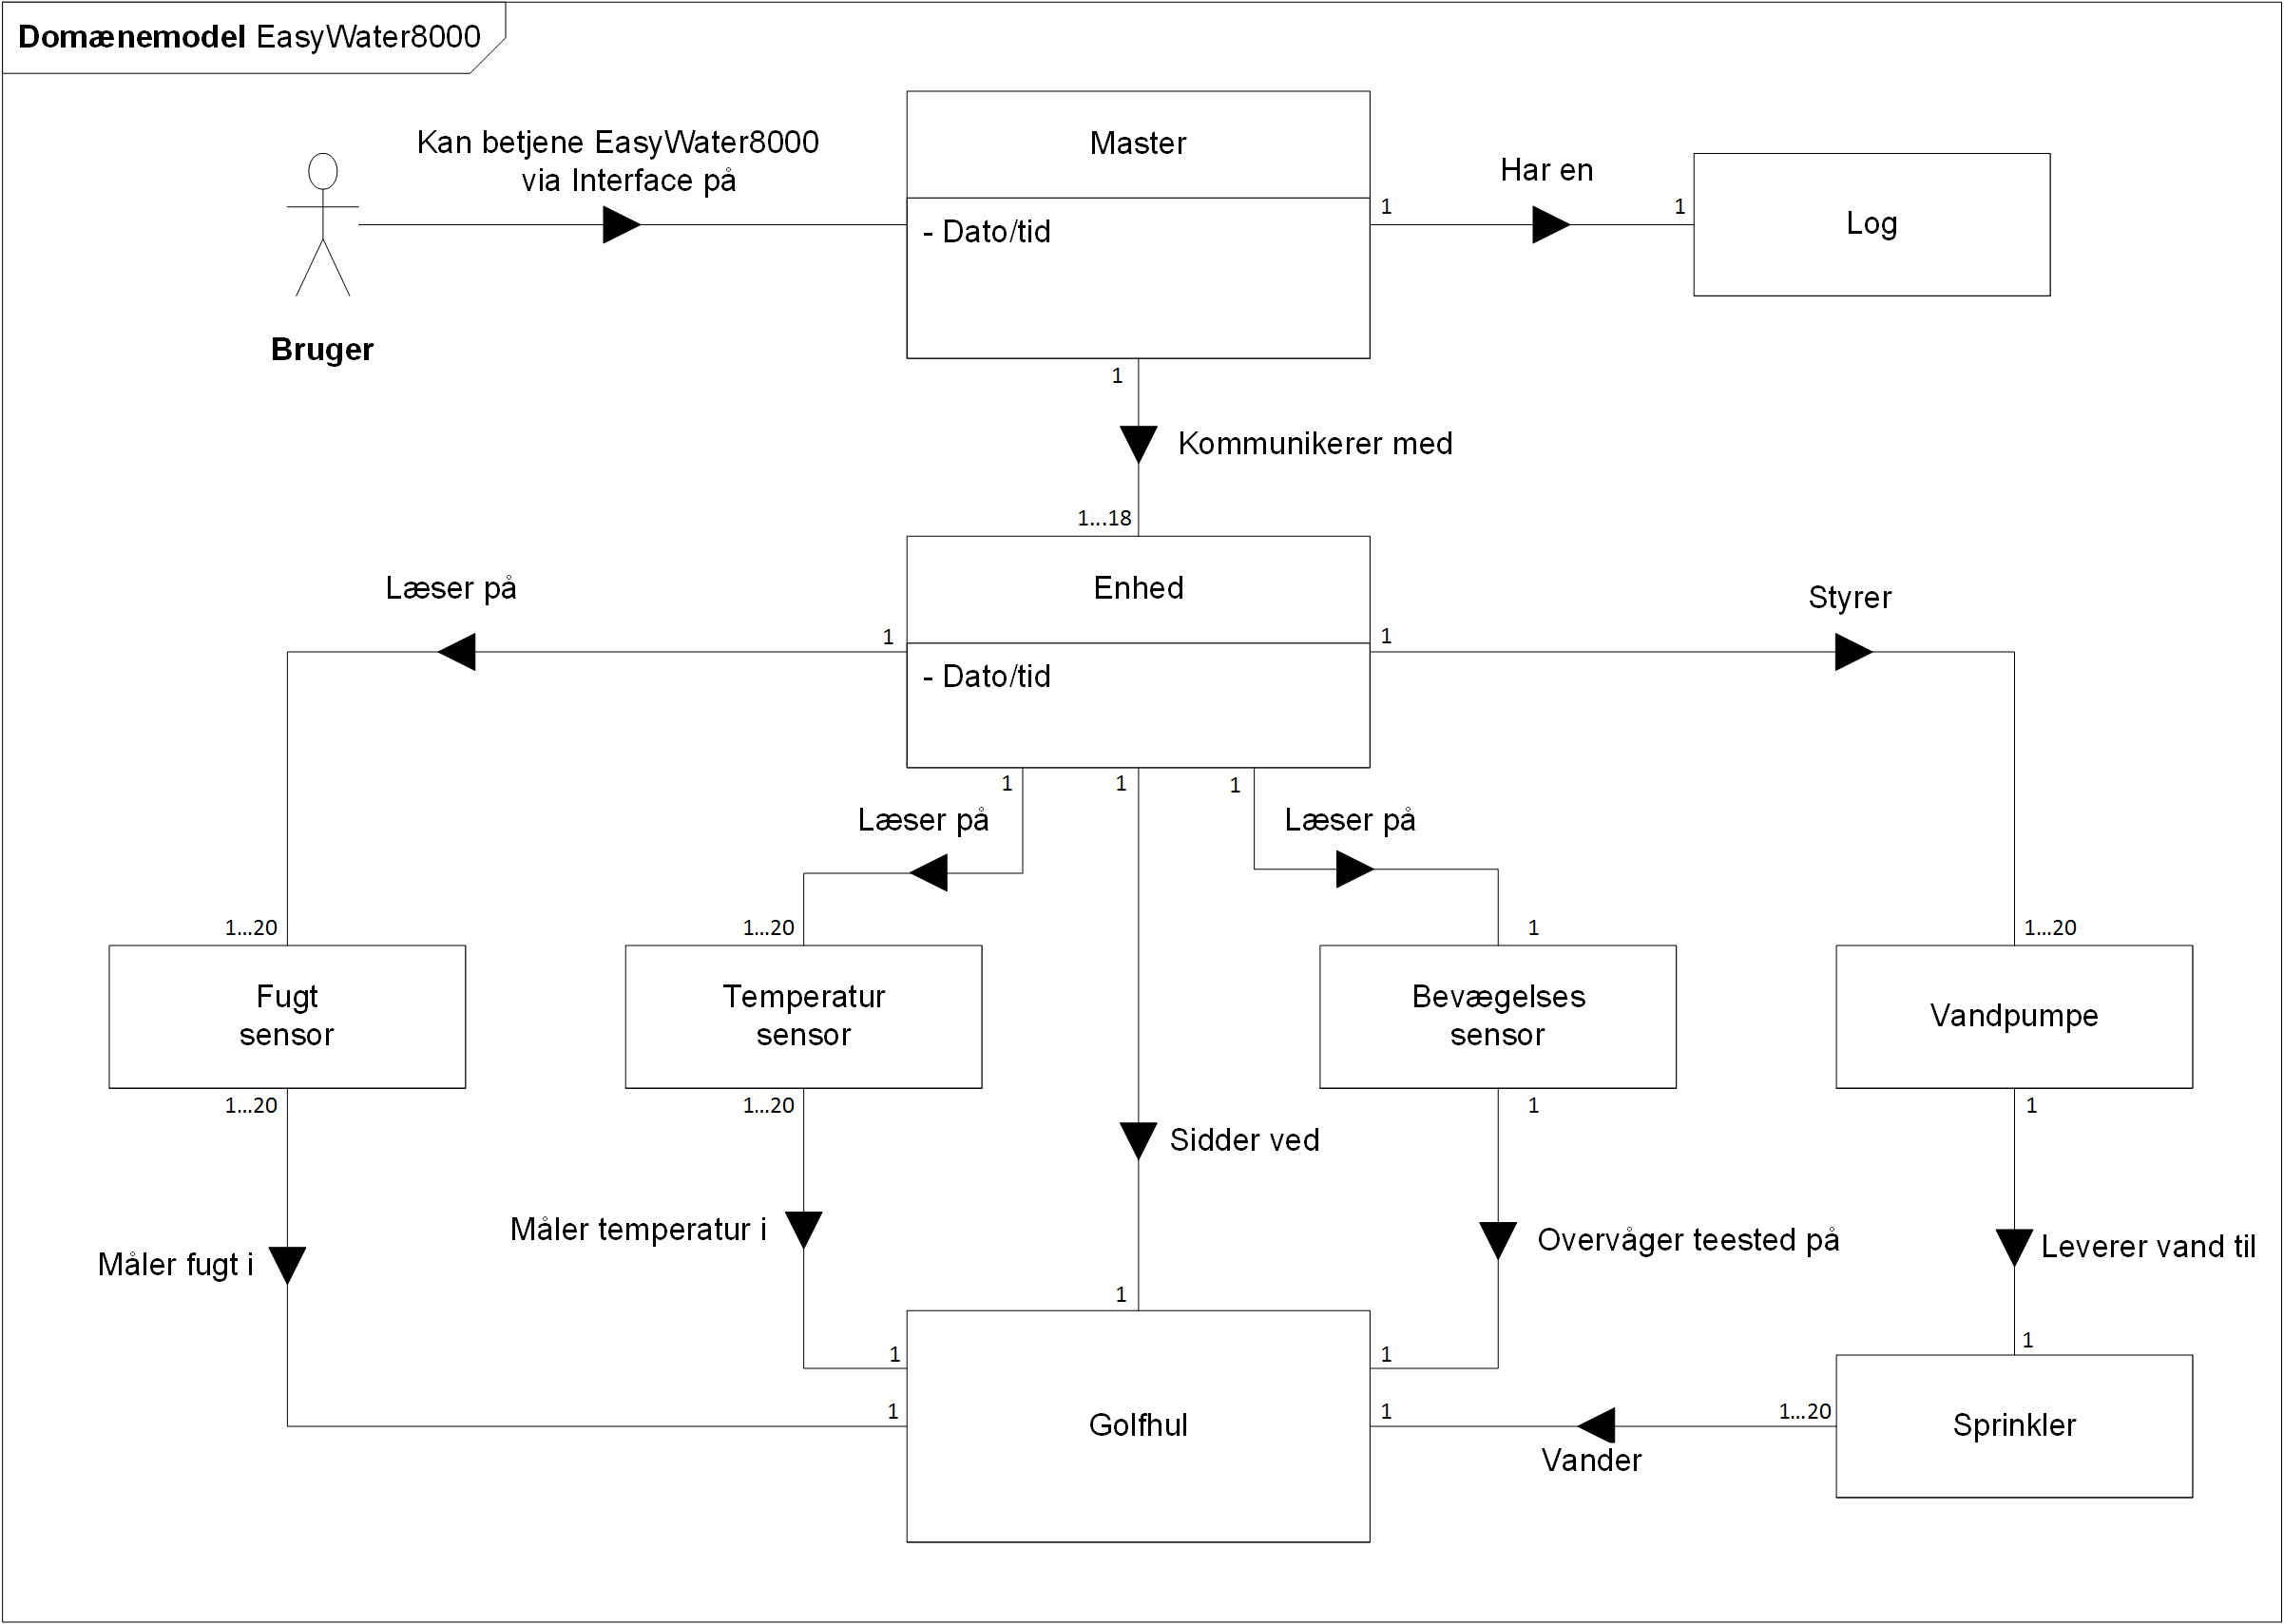
\includegraphics[width=\textwidth]{filer/systemarkitektur/Domainmodel}}
\caption{Domænemodel for EasyWater8000}
\label{lab:domainmodel}
\end{figure}
Domænemodellen i figur \ref{lab:domainmodel} beskriver EasyWater8000 systemets funktionalitet og de forskellige deles indbyrdes sammenhæng. 

\newpage
%% Hardware
\section{Hardware beskrivelse (HW)}
\begin{figure}[H] \centering
\subsection{BDD}
{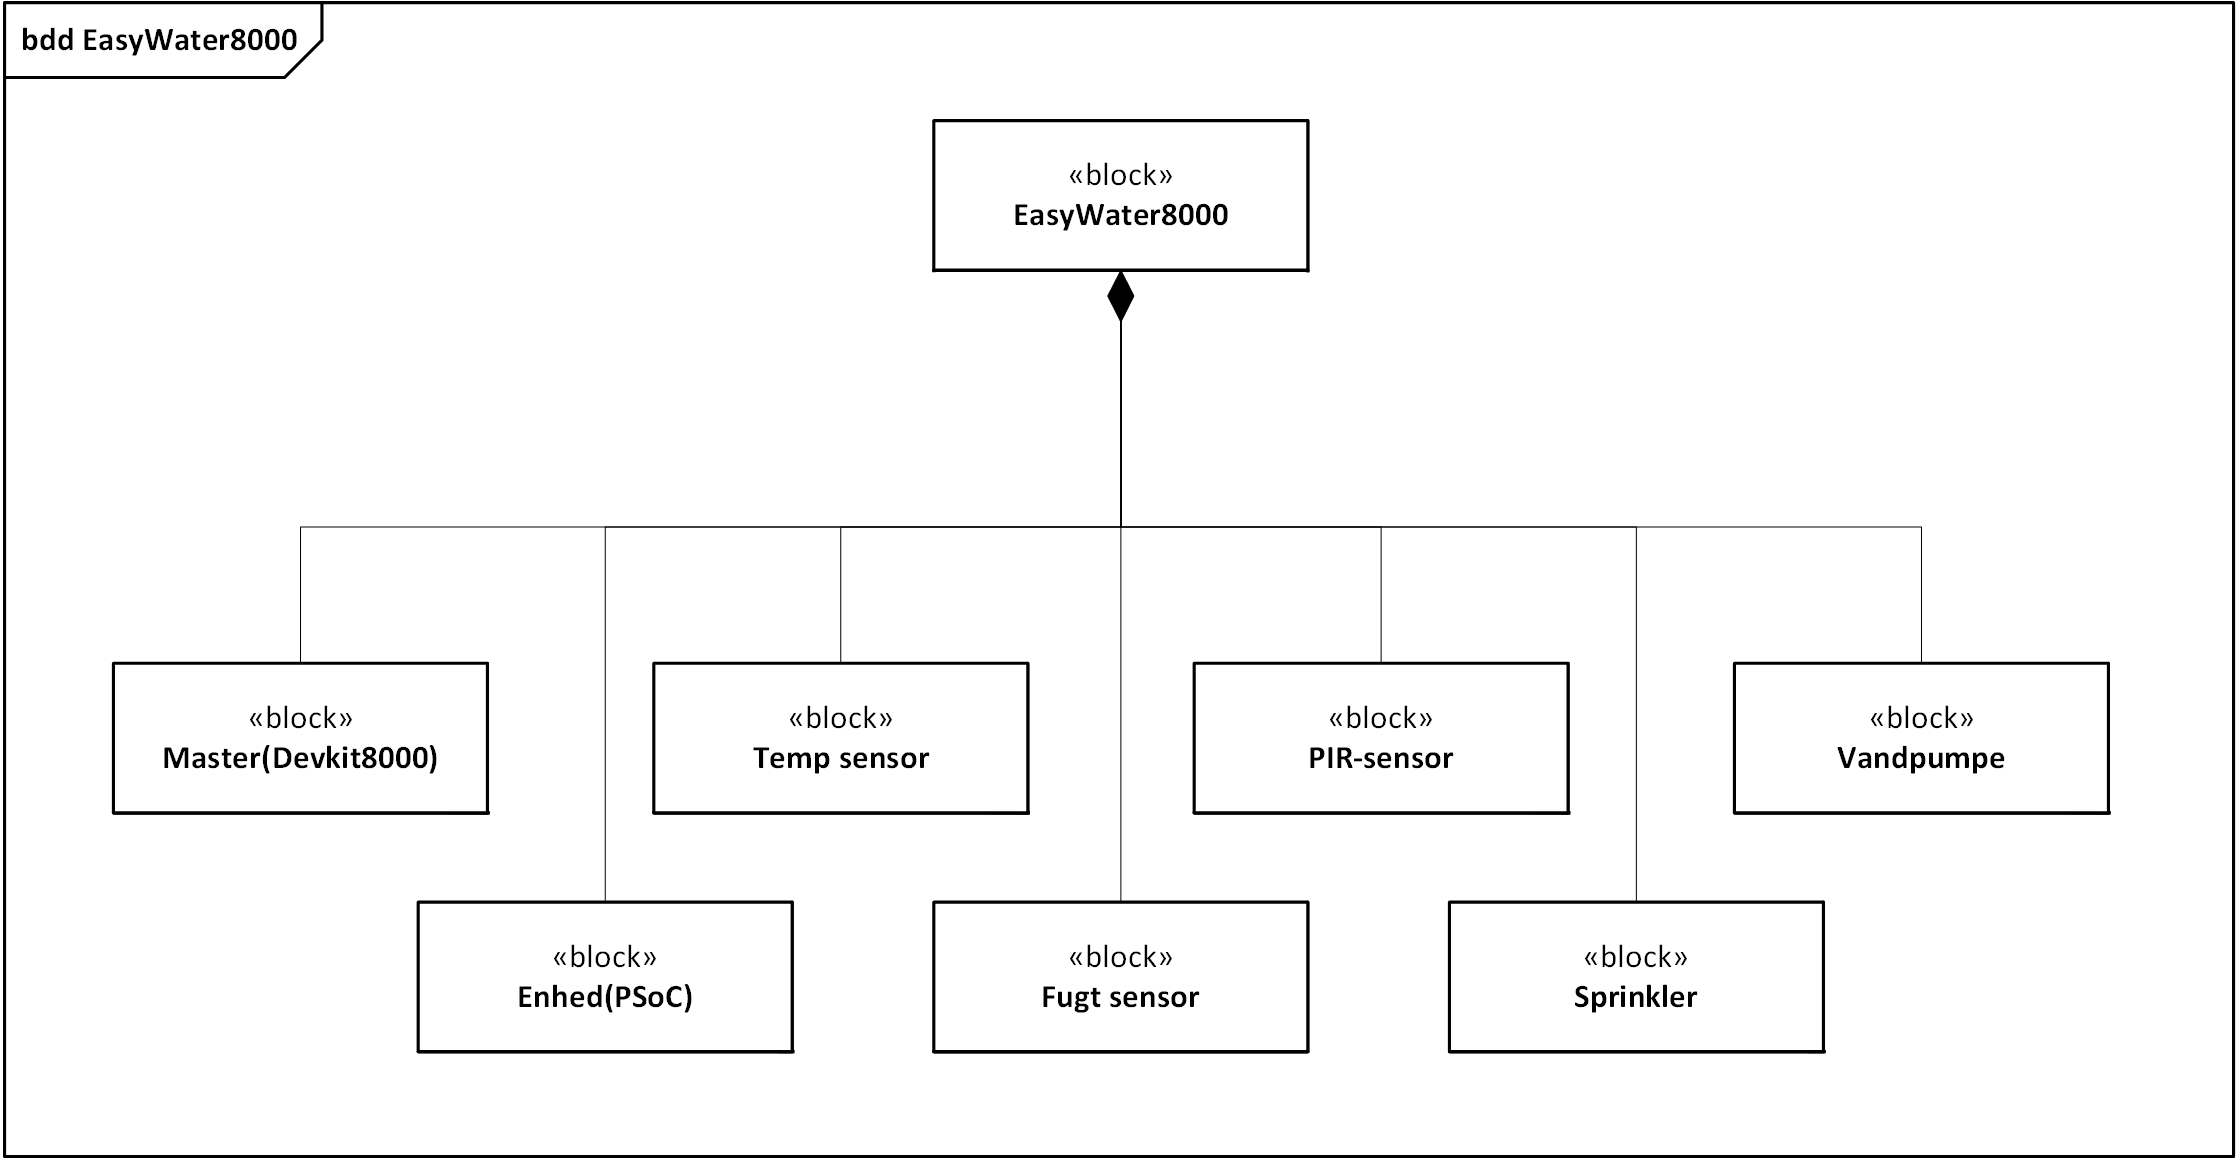
\includegraphics[width=0.9\textwidth]{filer/systemarkitektur/BDD}}
\caption{BDD for EasyWater8000}
\label{lab:bdd}
\raggedright
\end{figure}
BDD diagrammet giver et overblik over hvad det samlede EasyWater8000 system består af, samt indbyrdes multiplicitet. FT sensoren er en kombineret fugt- og temperatursensor.  \newline \newline

\begin{figure}[H] \centering
\subsection{BDD Master}
{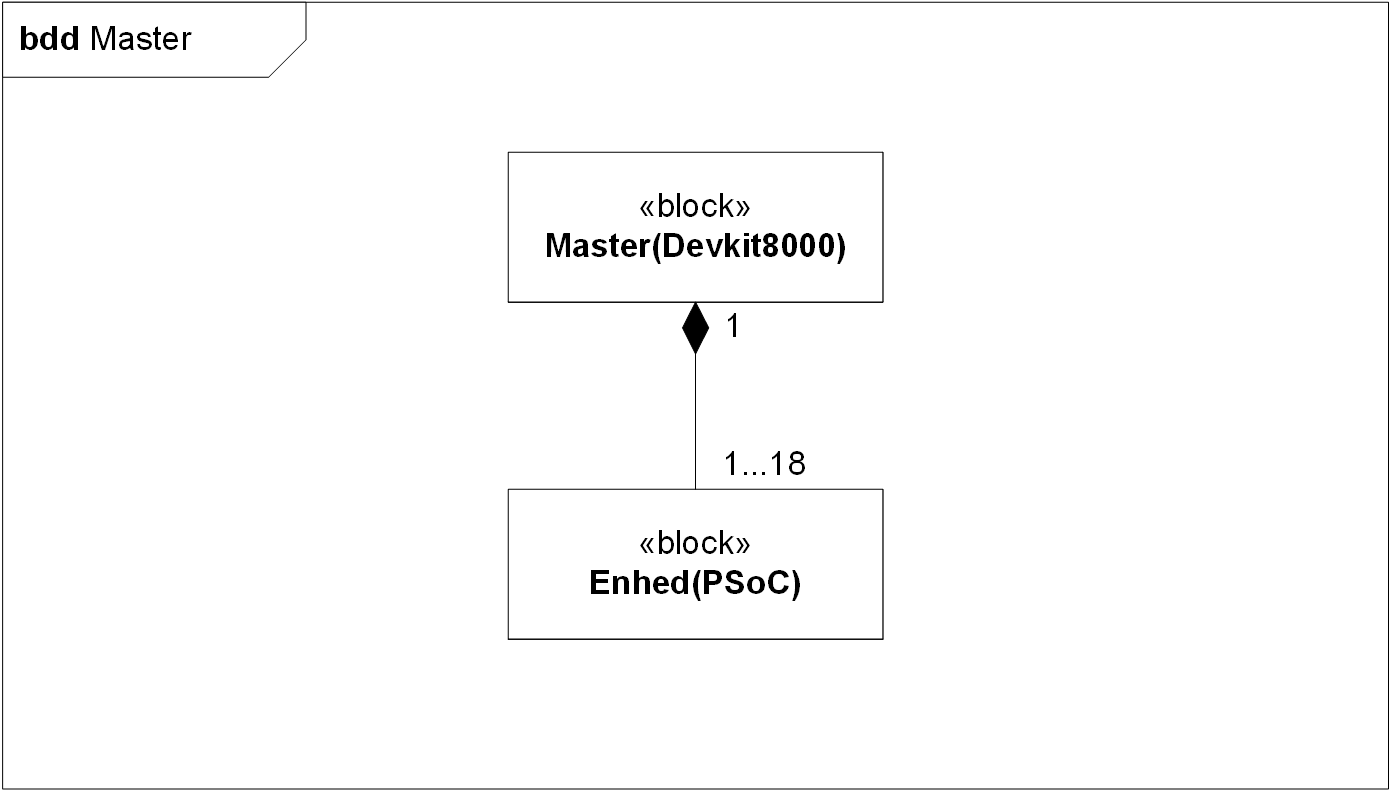
\includegraphics[width=0.7\textwidth]{filer/systemarkitektur/BDD_Master}}
\caption{BDD Master}
\label{lab:bddmaster}
\raggedright
\end{figure}
BDD diagrammet for Master, viser at Master består af ét Devkit8000, som kobles op med en til 18 Enheder.

\begin{figure}[H] \centering
\subsection{BDD Enhed}
{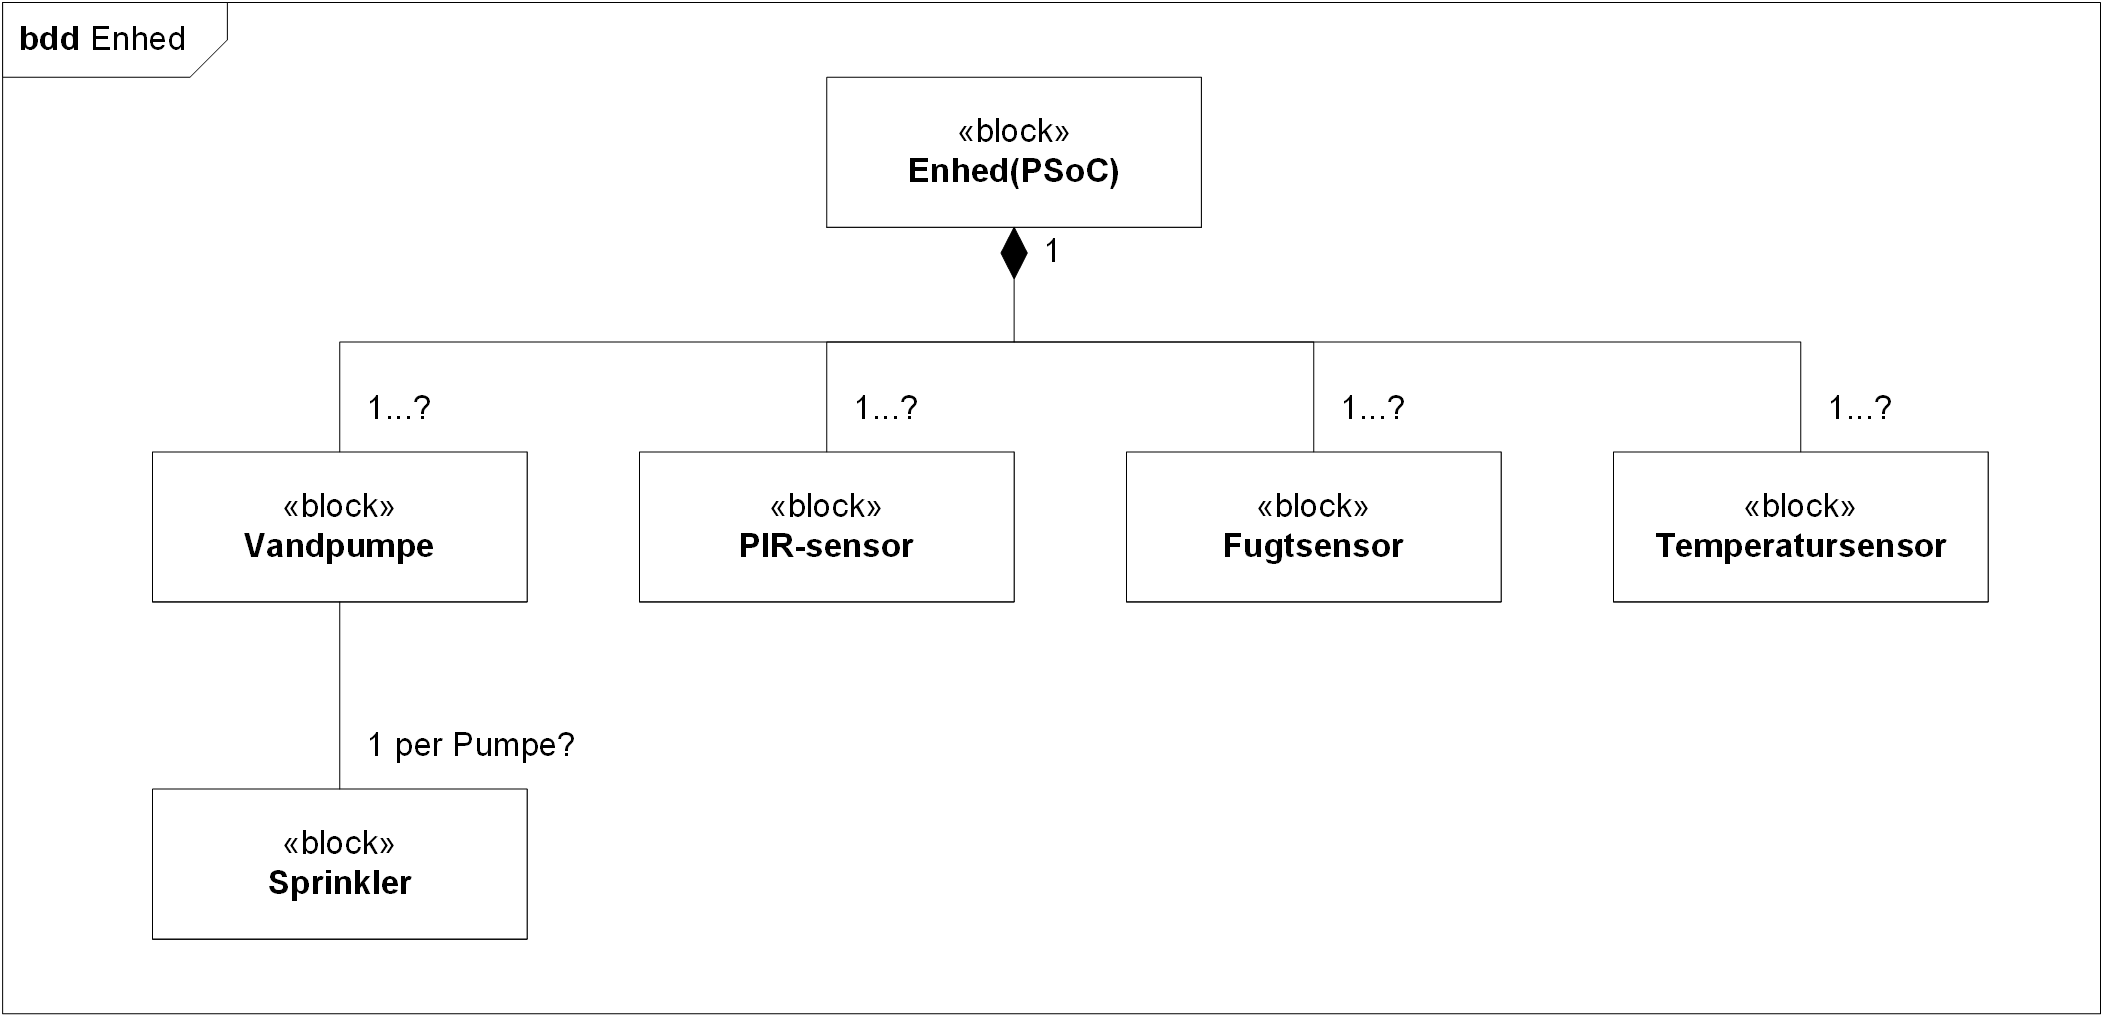
\includegraphics[width=0.9\textwidth]{filer/systemarkitektur/BDD_Enhed}}
\caption{BDD Enhed}
\label{lab:bddenhed}
\raggedright
\end{figure}

BDD diagrammet for Enhed, viser at én Enhed består af én PSoC som kan kobles sammen med op til 20 Vandpumper, 20 FT-sensorer samt 1 PIR-sensor. Sprinkleren bliver i systemet koblet sammen med én Vandpumpe.


\begin{figure}[H] \centering
\subsection{IBD}
{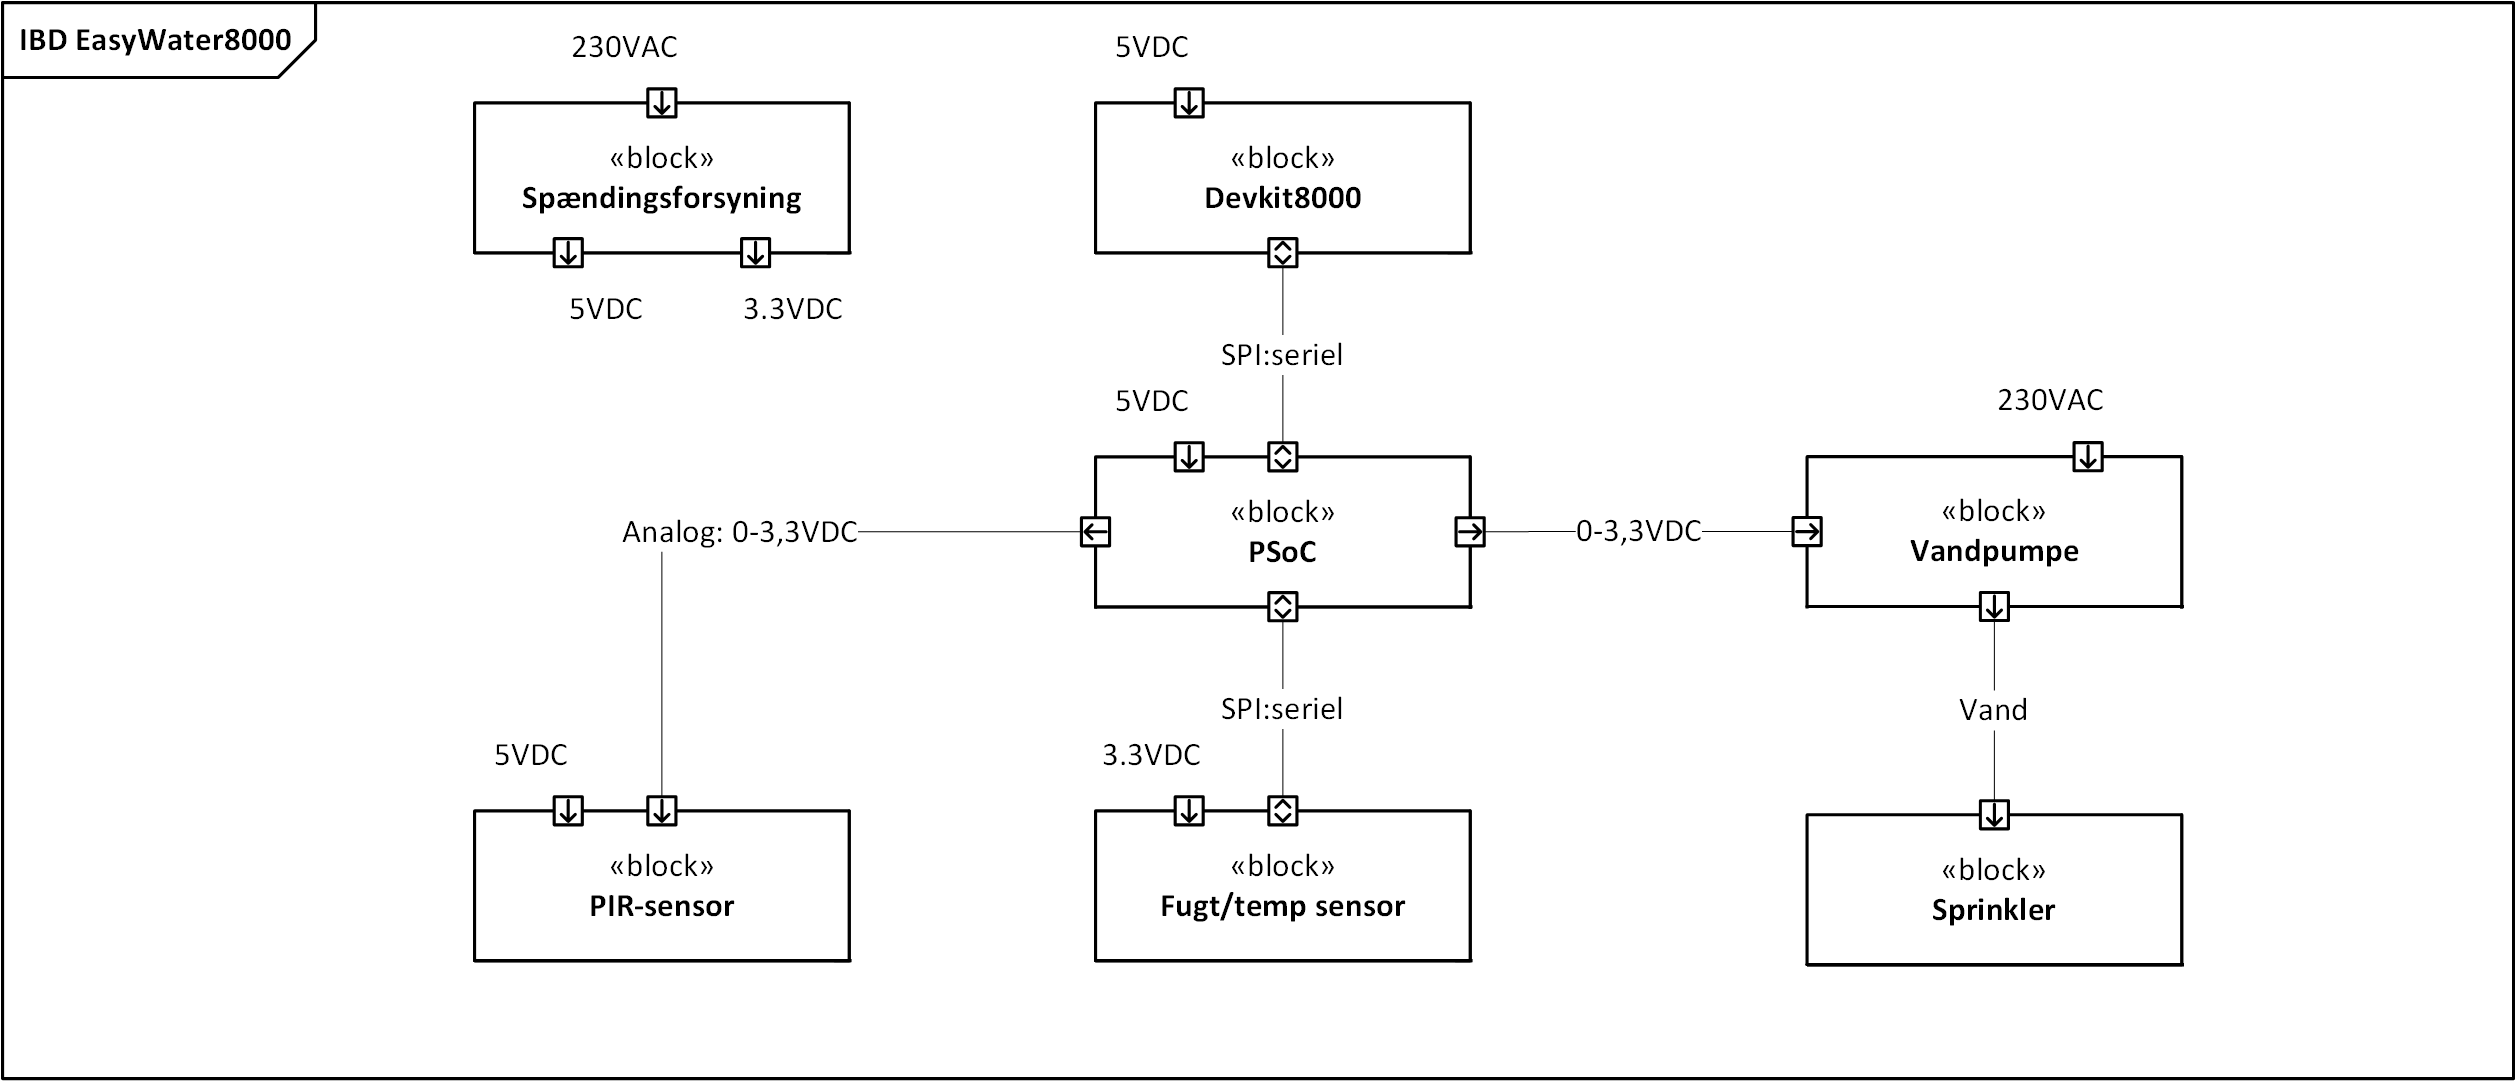
\includegraphics[width=0.9\textwidth]{filer/systemarkitektur/IBD}}
\caption{IBD for EasyWater8000}
\label{lab:ibd}
\raggedright
\end{figure}
IBD diagrammet giver et internt overblik over hvordan hele systemet er forbundet. Der ses hvilke typer signaler der bliver sendt imellem de forskellige blokke. \newline \newline
\textbf{Spændingsforsyning}: Spændingsforsyningens forbindelser er ikke påtegnet da dette ville give et uoverskueligt diagram, de er i stedet beskrevet med standardflowports. Spændingsforsyningen forsyner Enhed (PSoC4), FT sensor, PIR-sensor samt relæet i vandpumpen. Master (Devkit8000) har sin egen spændingsforsyning.  \newline \newline
\textbf{FT sensor}: Blokken beskriver at fugt- og temperatursensor er integreret i en chip. \newline \newline
\textbf{Relæ styring}: Blokken beskriver at vandpumpen består af et relæ, der står for at tænde/slukke for den. \newline \newline

\begin{table}[H] %% Blok og Signal Tabel
\subsection{Grænseflade}
For at opnå forståelse for signalerne mellem blokkene laves en grænseflade beskrivelse, der beskriver de enkelte blokkes porte og hvilke signaler der sendes imellem disse.

\subsubsection{Blok beskrivelse}
Til at beskrive blokkene nærmere anvendes tabel \ref{table:Bloktabel}. Her er hvert signal i en respektiv blok kommenteret og blokkens funktion er kort beskrevet. 

\caption{Tabel med beskrivelse af respektive blokke}
\begin{small}
\begin{tabular}{|p{3,3cm}|p{3,3cm}|p{3,3cm}|p{3,3cm}|}
\hline
\textbf{Bloknavn} & \textbf{Funktion} & \textbf{Signaler} & \textbf{Kommentar} \\ \hline

Master(Devkit8000) & Styreenhed der modtager input fra touchskærm og kommunikere serielt med Enhed(er) & Input:Touch & Masteren modtager inputs fra brugeren via touch \\ \cline{3-4}	
& 				   & SPI:SPI seriel & Seriel data kommunikation \\ \hline

Enhed(PSoC) & Enhed er grænsefladen til den fysiske verden igennem sensorer & SPI:SPI seriel & Seriel data kommunikation \\ \cline{3-4}
& & PIR-TTL 		& Signal fra PIR-sensor	\\ \cline{3-4}
& & VP-TTL 		& Signal til vandpumpe 	\\ \cline{3-4}
& & FT-TTL 		& Signal til FT-sensor 	\\ \cline{3-4}
& & FT-Analog 	& Signal fra FT-sensor 	\\ \hline

FT-sensor & Måler temperatur og fugt & FT-Analog & Analog signal til Enhed \\ \cline{3-4}
& & FT-TTL 	& Signal fra Enhed 	\\ \hline

PIR-sensor & Detekterer bevægelse & PIR-TTL & Signal til Enhed \\ \hline

Vandpumpe & Forsyner sprinkler med vand & Vand:Vand & Vand til sprinkler \\ \hline
 
Sprinkler & Fordeler vand på golfbane & Vand:Vand & Vand til golfbane \\ \hline

Spændingsforsyning & Forsyner EasyWater8000, Master har sin egen spændingsforsyning & Power:3,3VDC \newline Max strømbelastning: 3,4A & Forsyning til FT-sensor \\ \cline{3-4}
& & Power:5VDC \newline Max strømbelastning:2,2A		& Forsyning til PIR-sensor, Enhed 	\\ \hline
\end{tabular}
\end{small}
\label{table:Bloktabel}
\end{table}

\begin{table}[H]
\subsection{Signal beskrivelse}
For at fuldende beskrivelsen af grænsefladen er der lavet en signaltabel (tabel\ref{table:Signaltabel}). Hvert signal er beskrevet, og området et signal er defineret under, er også beskrevet. Blok og terminal indgår også. 
\caption{Tabel over signaler med terminaler}
\begin{small}
\begin{tabular}{|p{2cm}|p{2cm}|p{2cm}|p{2cm}|p{2cm}|p{2,2cm}|}
\hline

\textbf{Signal-navn}	&\textbf{Funktion} 		&\textbf{Område} &\textbf{Port 1} 	&\textbf{Port 2} 			&\textbf{Kommentar} \\ \hline

SPI:SPI seriel 			&Seriel kommunikation 	& 				&Master (DK\_02)		&Enhed (P\_DK)			&					 \\\hline

PIR-TTL 					&TTL 					&0(lav)\slash3,3V(høj) 	&PIR-sensor (PIR\_01) &Enhed (P\_PIR)			&Interrupt reagerer på høj flanke 					\\\hline
VP-TTL 					&TTL 					&0(lav)\slash3,3V(høj) 	&Enhed (P\_VP)  &Vandpumpe (VP\_01)				&					\\\hline
					
FT-TTL					&TTL						&0(lav)\slash3,3V(høj) 	&Enhed (P\_FT2) &FT-sensor (FT\_02)				&	    				\\\hline
FT-Analog				&Analog 					&0-3,3V 	\newline +/-10\%	&FT-sensor (FT\_01) &Enhed (P\_FT1)				& PWM signal	    				\\\hline

\end{tabular}
\end{small}
\label{table:Signaltabel}
\end{table}

\clearpage
%% Sowftware
\section{Software beskrivelse}
For at danne overblik over software-udviklingen inden det egentlige design laves bruges N+1 modellen.
Denne beskriver fire faser som tager hånd om de overordnede ting inden for software, alt sammen med use-cases som den røde tråd.
De fire fase er:
\begin{enumerate}
	\item Logical View
	\item Deployment View
	\item Implementation View
	\item Data View
\end{enumerate}

Ud over disse punkter tænkes der også en overordnet fejl-håndtering ind i projektet samt skitser for den grafiske brugerflade. Disse punkter er beskrevet i detaljer her efter.

\subsection{Logical View (JSA)}
%% SW arkitektur: Logical View

Logical View skal danne et overblik over hvilke softwarepakker der befinder sig på platforme. Blokkene inde i de respektive pakker kan sammen med domænemodellen, hjælpe med at give et overblik over hvilke klasser og kernemoduler der skal bruges.

\begin{figure}[htbp] \centering
{\includegraphics[scale=0.7]{filer/systemarkitektur/logical_view_devkit}}
\caption{Logical view for Devkit8000 illustrerer hvilke softwarepakker der befinder sig på Masteren }
\label{fig:Logical View Devkit8000}
\end{figure}

Figur \ref{fig:Logical View Devkit8000} illustrerer hvilke softwarepakker der ligger på Masteren. I bunden er \textit{Device drivers}-pakken som håndterer SPI kommunikationen imellem Master og Enhed. I midten ligger \textit{Hardware API}-pakken som håndterer protokol-vedtægter ifm. kommunikationen. \textit{Application}-pakken tager sig af alt UI samt log og fejlhåndtering.

\clearpage

\newenvironment{figure1}[1][]{\begin{figure}[#1]\vspace{3.0cm}}{\vspace{1.0cm}\end{figure}}
\begin{figure1}[htbp] \centering
{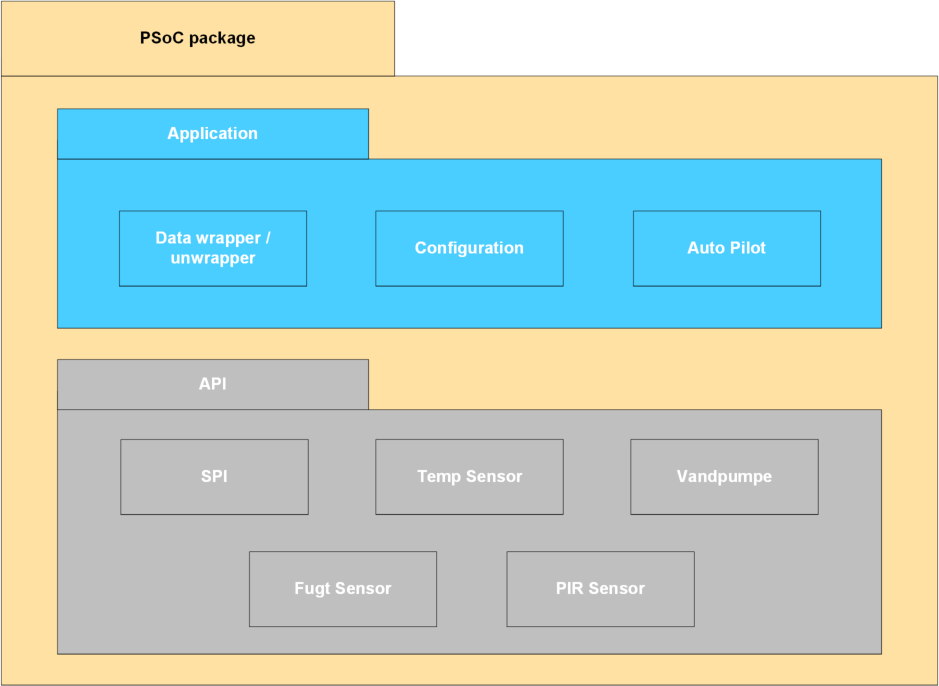
\includegraphics[scale=0.7]{filer/systemarkitektur/logical_view_psoc}}
\caption{Logical view for PSoC illustrer hvilke software pakker der befinder sig på enhederne}
\label{fig:Logical View PSoC}
\end{figure1}

Figur \ref{fig:Logical View PSoC} illustrerer hvilke softwarepakker der ligger på Enhederne. \textit{API}-pakken består af den software som håndterer hardwaren, dvs. den tager imod input og får formateret det til noget brugbart for \textit{Application}-pakken. \textit{Application}-pakken håndterer den indsamlede data som den får fra sensorene igennem \textit{API}-pakken. Denne data sammensættes iht. protokollen og sendes til API pakken som får det sendt til Devkit8000. Pakken skal også håndterer data fra Devkit8000 til at konfigurerer de parametre der styrer automatiseringen af vandingen.



\subsection{Deployment View ()}
%% SW arkitektur: Deployment View

Deployment view skal illustrere hvor hvilke lag af software ligger på vores platforme. Devkit8000 kører linux og har derfor flere software lag end PSoC'en.
 
\vspace{15 mm}

\begin{figure}[htbp] \centering
{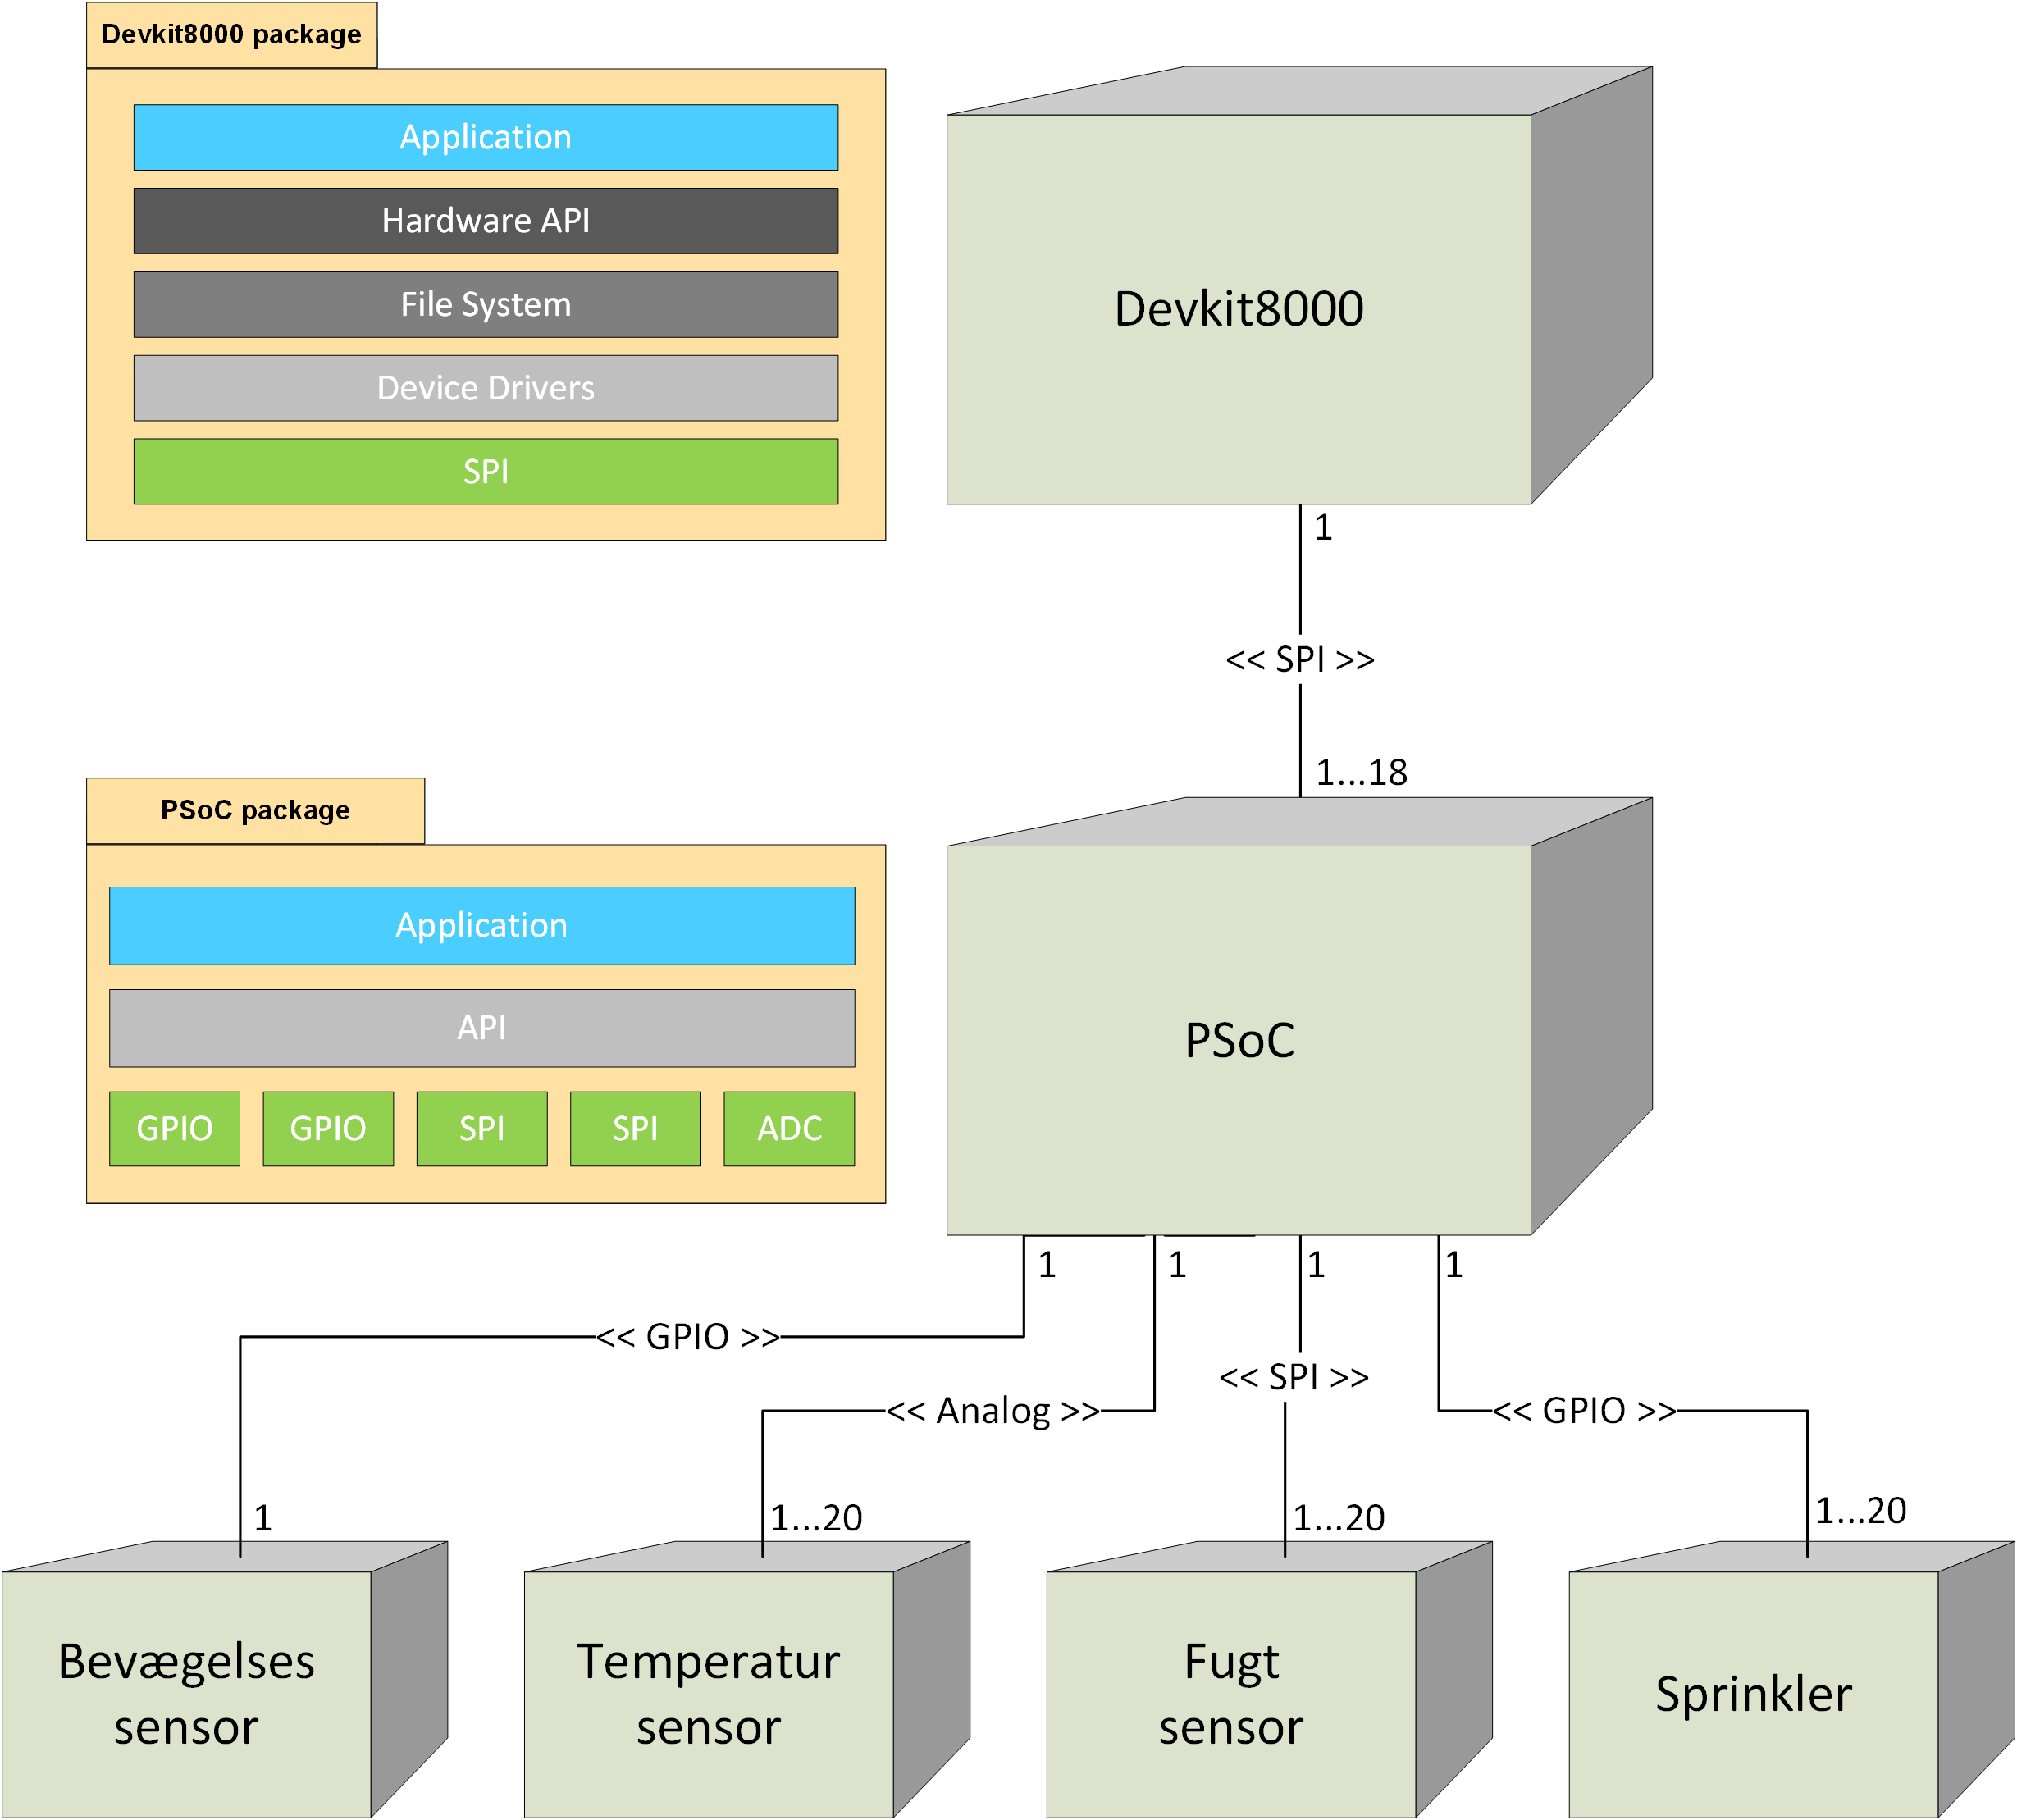
\includegraphics[scale=0.7]{filer/systemarkitektur/Deployment_model}}
\caption{Deployment model illustrere de forskellige software og hardware(grønne) lag}
\label{fig:Deployment Model}
\end{figure}

\vspace{5 mm}

\subsubsection{Devkit8000}
\textit{Applications} laget består af alt den software som har med brugeren at gøre, dvs. UI og tilhørende controllers. Applicationslaget tager imod input fra brugeren og reagere på det enten ved at kalde nogle af sine egne controllers eller sende kommandoer til hardware APIen. Laget skal desuden få data fra nedenstående lag til at fremstå overskueligt over for brugeren.

\clearpage

\textit{Hardware API} laget består af almindelige klasser som gør brug af file systemets kommandoer som f.eks open og close.

\textit{File System}

\textit{Device Driver} laget består af den software som håndtere alt hardware input og output. Hardware proxys inklusiv.

\textit{HW connection (grønne bokse)} laget viser hvilke hardware in/out der er til devkittet

\subsubsection{PSoC}

\textit{Applications} laget håndtere den indsamlede data som den får fra sensorene igennem API'en. Denne data sammensættes ifølge protokollen og sendes til API'en som får det sendt til devkittet. Laget skal også håndtere data fra devkittet til at konfigurere de parametre der styre automatiseringen af vandingen som applications laget også håndtere.

\textit{API} laget består af den software som håndtere hardwaren. dvs den tager imod input og får formateret det til noget læseligt til applications laget. Derudover står den for at få sendt de informationer applicationslaget ber om på en effektiv og sikker måde.

\textit{HW connection (grønne bokse)} laget viser hvilke hardware in/out der er til PSoC'en

\subsection{Implementation View ()}
%% SW arkitektur: Implementation View

Inden programmerne designes, fastlægges en struktur for kildekoden. På den måde er det nemmere for flere programmører at arbejde med delene i programmet samtidigt.

Strukturen skal være som vist i figur \ref{fig:implementationview}. Under mappen ''Kildekode'' skal hver klasse have en mappe med dertil hørende filer. Ligeledes med ''Testprogrammer'' mappen, som indholder testprogrammer som verificerer funktionaliteten af de enkelte moduler.
Mappen ''Kompilerede programmer'' er til de endelige programmer.

\begin{figure}[htbp] \centering
{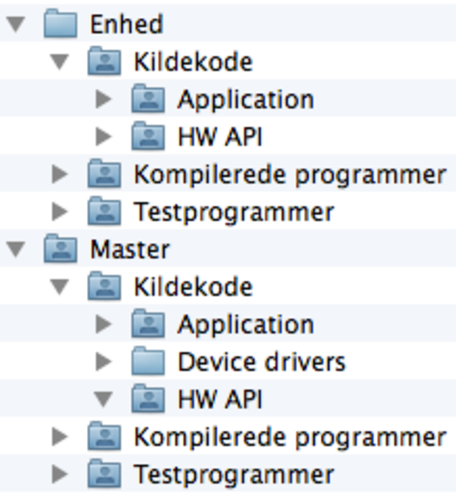
\includegraphics[scale=0.7]{filer/pics/SW-Implementation-View}}
\caption{Mappestruktur for software-kilder}
\label{fig:implementationview}
\end{figure}

\subsection{Data View (BS)}
%% SW arkitektur: Data View

I forbindelse med EasyWater8000s log skal der gemmes data på en nem og håndterbar måde. Det skal være muligt at gemme følgende data:

\begin{enumerate}
	\item Tidsstempel
	\item Temperatur
	\item Fugtighed
	\item Bevægelse
	\item Vanding
\end{enumerate}

Ydermere skal disse informationer gemmes for hver Enhed. Så hvis der er 18 huller med i alt 18 Enheder, skal ovenstående gemmes for alle 18 enheder.

Når informationen skal præsenteres for brugeren skal det ske i en tabel som vist på figur \ref{fig:GUI-log-alle} i afsnit \ref{subsec:GUI}, data for en enkelt enhed som på figur \ref{fig:GUI-log-enhed} i afsnit \ref{subsec:GUI} eller på en graf så man kan se ændringer over tid som vist på figur \ref{fig:log-graf}.

\begin{figure}[htbp] \centering
{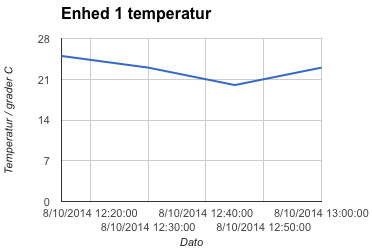
\includegraphics[scale=0.5]{filer/pics/SW-Log-graf}}
\caption{Graf for temperatur for én Enhed}
\label{fig:log-graf}
\end{figure}

Tabellen skal have en fane for hver opkoblet Enhed. Her kan man se informationer fra hver enkelt Enhed. Det bør også være muligt at se alle enheders informationer samtidigt.

Dataen struktureres i semikolon-separerede filer (\verb+.csv+) på Master. Hver Enhed har en fil hvor alle data er samlet med udgangspunkt i strukturen vist i liste \ref{list:log-csv-struktur}.

\begin{lstlisting}[caption=Semikolon-separeret datafil til log af enheder, label={list:log-csv-struktur}]
<enheds-nr>;
<KP-nr>; <dato>; <temperatur>; <fugtighed>; <bevaeglse>; <vanding>;
<KP-nr>; <dato>; <temperatur>; <fugtighed>; <bevaeglse>; <vanding>;
...
<KP-nr>; <dato>; <temperatur>; <fugtighed>; <bevaeglse>; <vanding>;
\end{lstlisting}

Dette resulterer i en filstruktur som vist på liste \ref{list:log-fil-struktur} hvis der er koblet 18 Enheder op på Master.

\begin{lstlisting}[caption=Filstruktur for logfiler på Master, label={list:log-fil-struktur}]
<log>/
  <enheds-nr1>.csv
  <enheds-nr2>.csv
  ...
  <enheds-nr17>.csv
  <enheds-nr18>.csv
\end{lstlisting}

Hyppigheden for målingerne og logningen er beskrevet i de ikke-funktionelle krav, \ref{header:ikke-funk}.


\subsection{Fejl-håndtering (JC)}
%% SW arkitektur: Fejlhåndtering

Systemet kan håndterer fejl og disse vil blive gemt i en fejllog som bliver gemt på Master. 

Fejlhåndteringen bliver klaret af en klasse på Devkit8000 som håndterer at skrive det rigtige fejl ud i en \verb+.txt+-fil. Klassen vil blive kaldt med en fejlkode hver gang fejl opstår. Klassen forstår så at skrive den rigtige fejl ind i txt filen ud fra den pågældende fejlkode den har modtaget som attribut. 

Alle funktioner vil returnere et negativt heltal som repræsenterer en fejlkoden som klassen kan tolke på.

\begin{figure}[htbp] \centering
{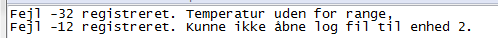
\includegraphics[scale=0.7]{filer/pics/Errortxt}}
\caption{udsnit af Error log}
\label{fig:ErrorLog}
\end{figure}

Billedet på figur \ref{fig:ErrorLog} viser hvordan 2 fejl i error-loggen kunne se ud.

\subsection{Grafiske brugerflade-skitser (BS)}
\label{subsec:GUI}
%% SW arkitektur: GUI skitser

Inden det endelige GUI udvikles laves nogle skitser som udviklingen læner sig op af. Ud fra UC beskrivelserne findes de skærmbilleder som skal vises på Master og skitseres.

Her følger korte beskrivelser af hver skitse samt skitsen selv.

\subsubsection{Startmenu}
Figur \ref{fig:GUI-Startmenu} er den første menu brugeren kommer til. Her er valgmulighederne præsenteret for brugeren.

\begin{figure}[htbp] \centering
{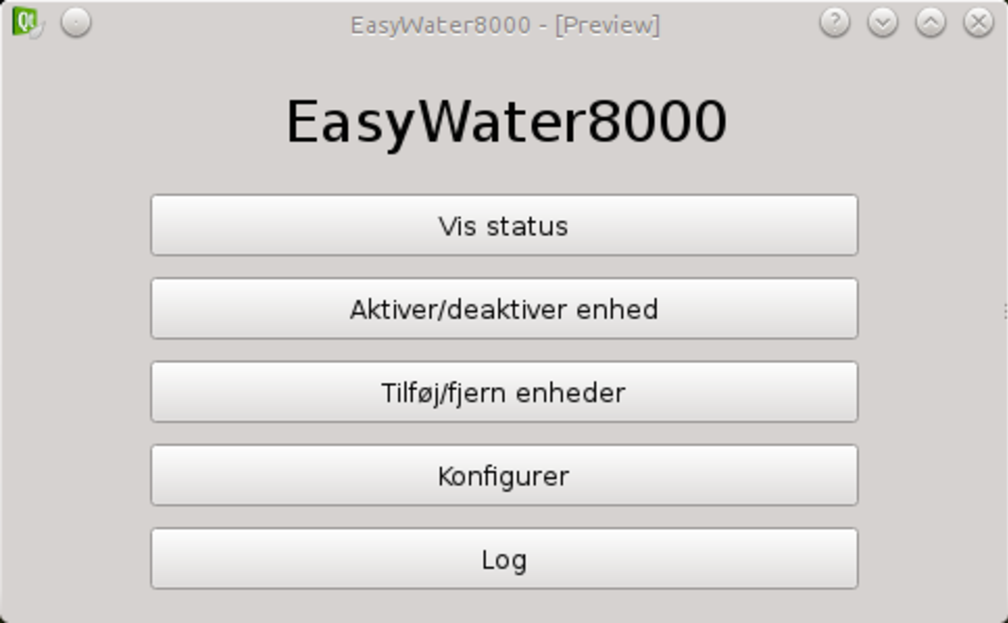
\includegraphics[scale=0.5]{filer/pics/GUI/Start-menu}}
\caption{Skitse af startmenu på GUI}
\label{fig:GUI-Startmenu}
\end{figure}

\subsubsection{Vis Status}
På figur \ref{fig:GUI-aktuel-status} vises den aktuelle status af systemets enheder. Den øverste række tal er tilkoblede Enheder. Den anden række tal er komponentpakker tilkoblet den enkelte enhed.

\begin{figure}[htbp] \centering
{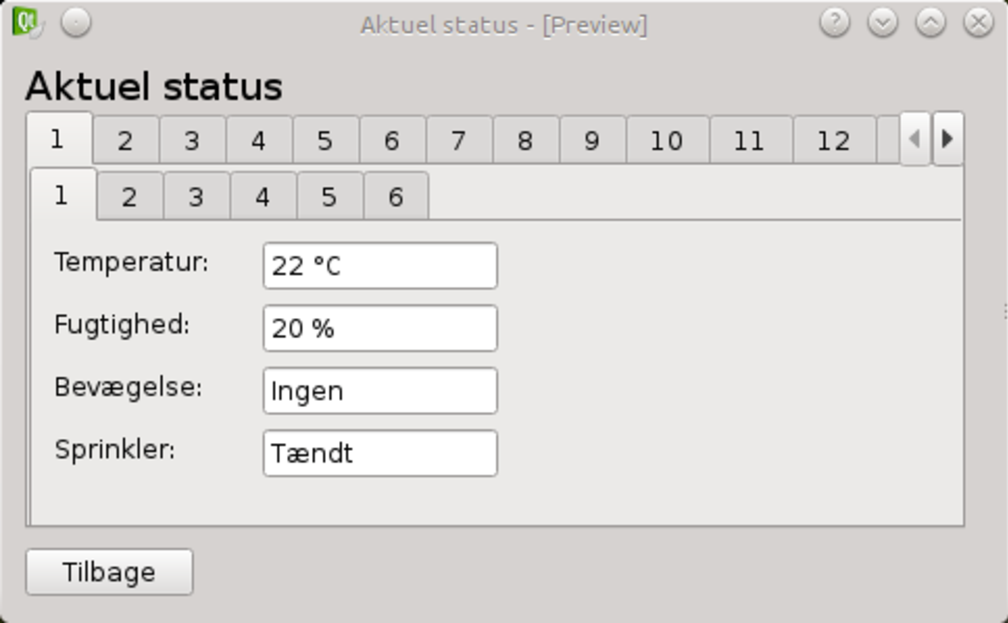
\includegraphics[scale=0.5]{filer/pics/GUI/Aktuel-status}}
\caption{Skitse af ''Vis status'' på GUI}
\label{fig:GUI-aktuel-status}
\end{figure}

\subsubsection{Aktiver og deaktiver enhed}
Skitsen på figur \ref{fig:GUI-aktiver-deaktiver} viser brugerens mulighed for at aktivere og deaktivere enkelte enheder i systemet.

\begin{figure}[htbp] \centering
{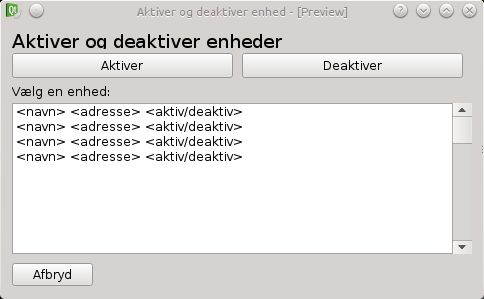
\includegraphics[scale=0.5]{filer/pics/GUI/Aktiver-deaktiver-enheder}}
\caption{Skitse af ''Aktiver og deaktiver enhed'' på GUI}
\label{fig:GUI-aktiver-deaktiver}
\end{figure}

\subsubsection{Tilføj/fjern enheder}
De præsenterede muligheder i forbindelse med at fjerne og tilføje enheder til systemet er vist på figur \ref{fig:GUI-tilfoj-fjern}.

\begin{figure}[htbp] \centering
{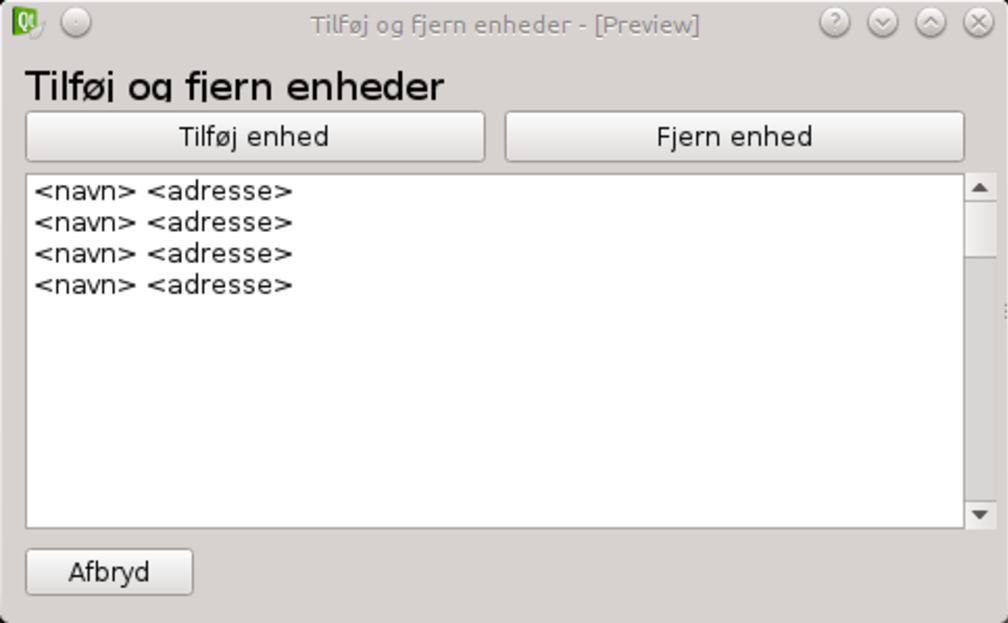
\includegraphics[scale=0.5]{filer/pics/GUI/Tilfoj-fjern-enheder}}
\caption{Skitse af ''Tilføj/fjern enheder'' på GUI}
\label{fig:GUI-tilfoj-fjern}
\end{figure}

\subsubsection{Konfigurer}
Når brugeren skal konfigurerer en enhed bruges skitsen på figur \ref{fig:GUI-konfigurer}. Her vælger brugeren hvilken enhed der skal konfigureres.

\begin{figure}[htbp] \centering
{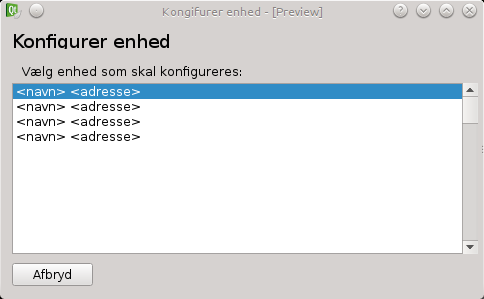
\includegraphics[scale=0.5]{filer/pics/GUI/Konfigurer-enhed}}
\caption{Skitse af ''Konfigurer'' på GUI}
\label{fig:GUI-konfigurer}
\end{figure}

\subsubsection{Indstil parametre}
Når brugeren har valgt en enhed som skal konfigureres vises skærmen på figur \ref{fig:GUI-indstil-parametre}. Her kan brugeren indtaste parametrene for enheden.

\begin{figure}[htbp] \centering
{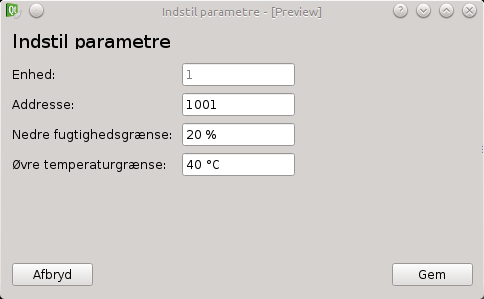
\includegraphics[scale=0.5]{filer/pics/GUI/Indstil-parametre}}
\caption{Skitse af ''Indstil parametre'' på GUI}
\label{fig:GUI-indstil-parametre}
\end{figure}

\subsubsection{Log}
Loggen præsenterer de indsamlede data fra alle enhederne. Det er muligt at se alle data på en gang, som vist på figur \ref{fig:GUI-log-alle}, hvor den øverste fanerække er numre på opsatte enheder i systemet, eller man kan vælge de enkelte enheder og se deres forskellige komponentpakker, som vist på figur \ref{fig:GUI-log-enhed}, hvor den anden fanerække er komponentpakker koblet op på systemet.

\begin{figure}[htbp] \centering
{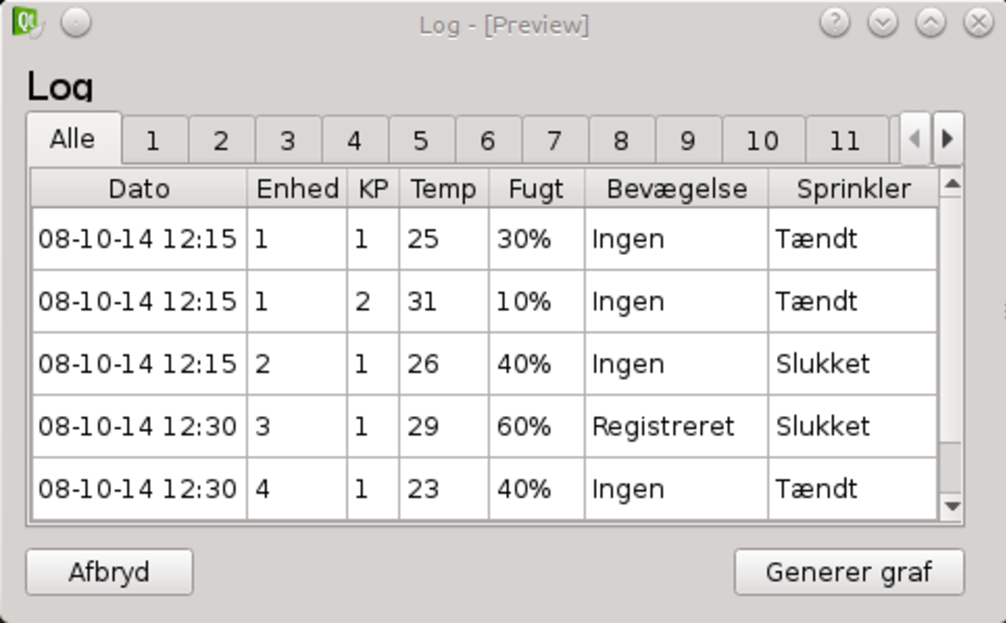
\includegraphics[scale=0.5]{filer/pics/GUI/Log-alle}}
\caption{Skitse af ''Log'' for alle enheder på GUI}
\label{fig:GUI-log-alle}
\end{figure}

\begin{figure}[htbp] \centering
{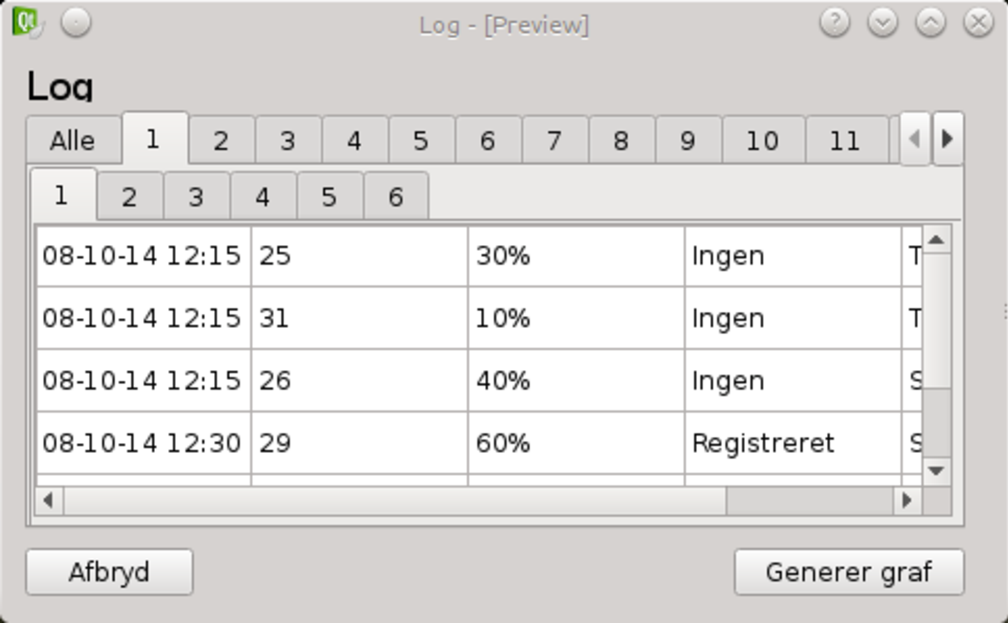
\includegraphics[scale=0.5]{filer/pics/GUI/Log-enhed}}
\caption{Skitse af ''Log'' for enkelt enhed på GUI}
\label{fig:GUI-log-enhed}
\end{figure}






%  Design - sections af HW og SW

\chapter{Design}

%HW
\chapter{Hardwaredesign}

\section{Prototypemodel}
Hardwaredesignet tager udgangspunkt i den ønskede prototype, der beskrives herunder.

Prototypen skal bestå af en Master (DevKit8000) der via SPI kommunikerer med én Enhed (PSoC4). Denne enhed har koblet én komponentpakke, bestående af én PIR-sensor (HC-SR501), én kombineret fugt,- og temperatursensor (SHT21P), én 230V/5V relæstyring, én vandpumpe (Alpha2) samt én sprinkler (Hunter PS).

Prototypen sætter herved begrænsninger i forhold til ovenstående beskrivelser af systemarkitekturen.

De enkelte dele af prototypen designes herunder.   




\section{FT-sensor (JS LB)}
Implementeringen af sht21p er sket ved at designe et print som indeholder sht21p og et 2. ordensfilter. 
Da sht21p-komponentet er et SMD-komponent var det ikke muligt at opstille kredsløbet på vero-board. Det var derfor nødvendigt at få et print produceret. Til design af printet blev CadSoft EAGLE PCB design software brugt. Nedenfor ses diagram og PCB layout af printet.


\begin{figure}[htb]
\centering
{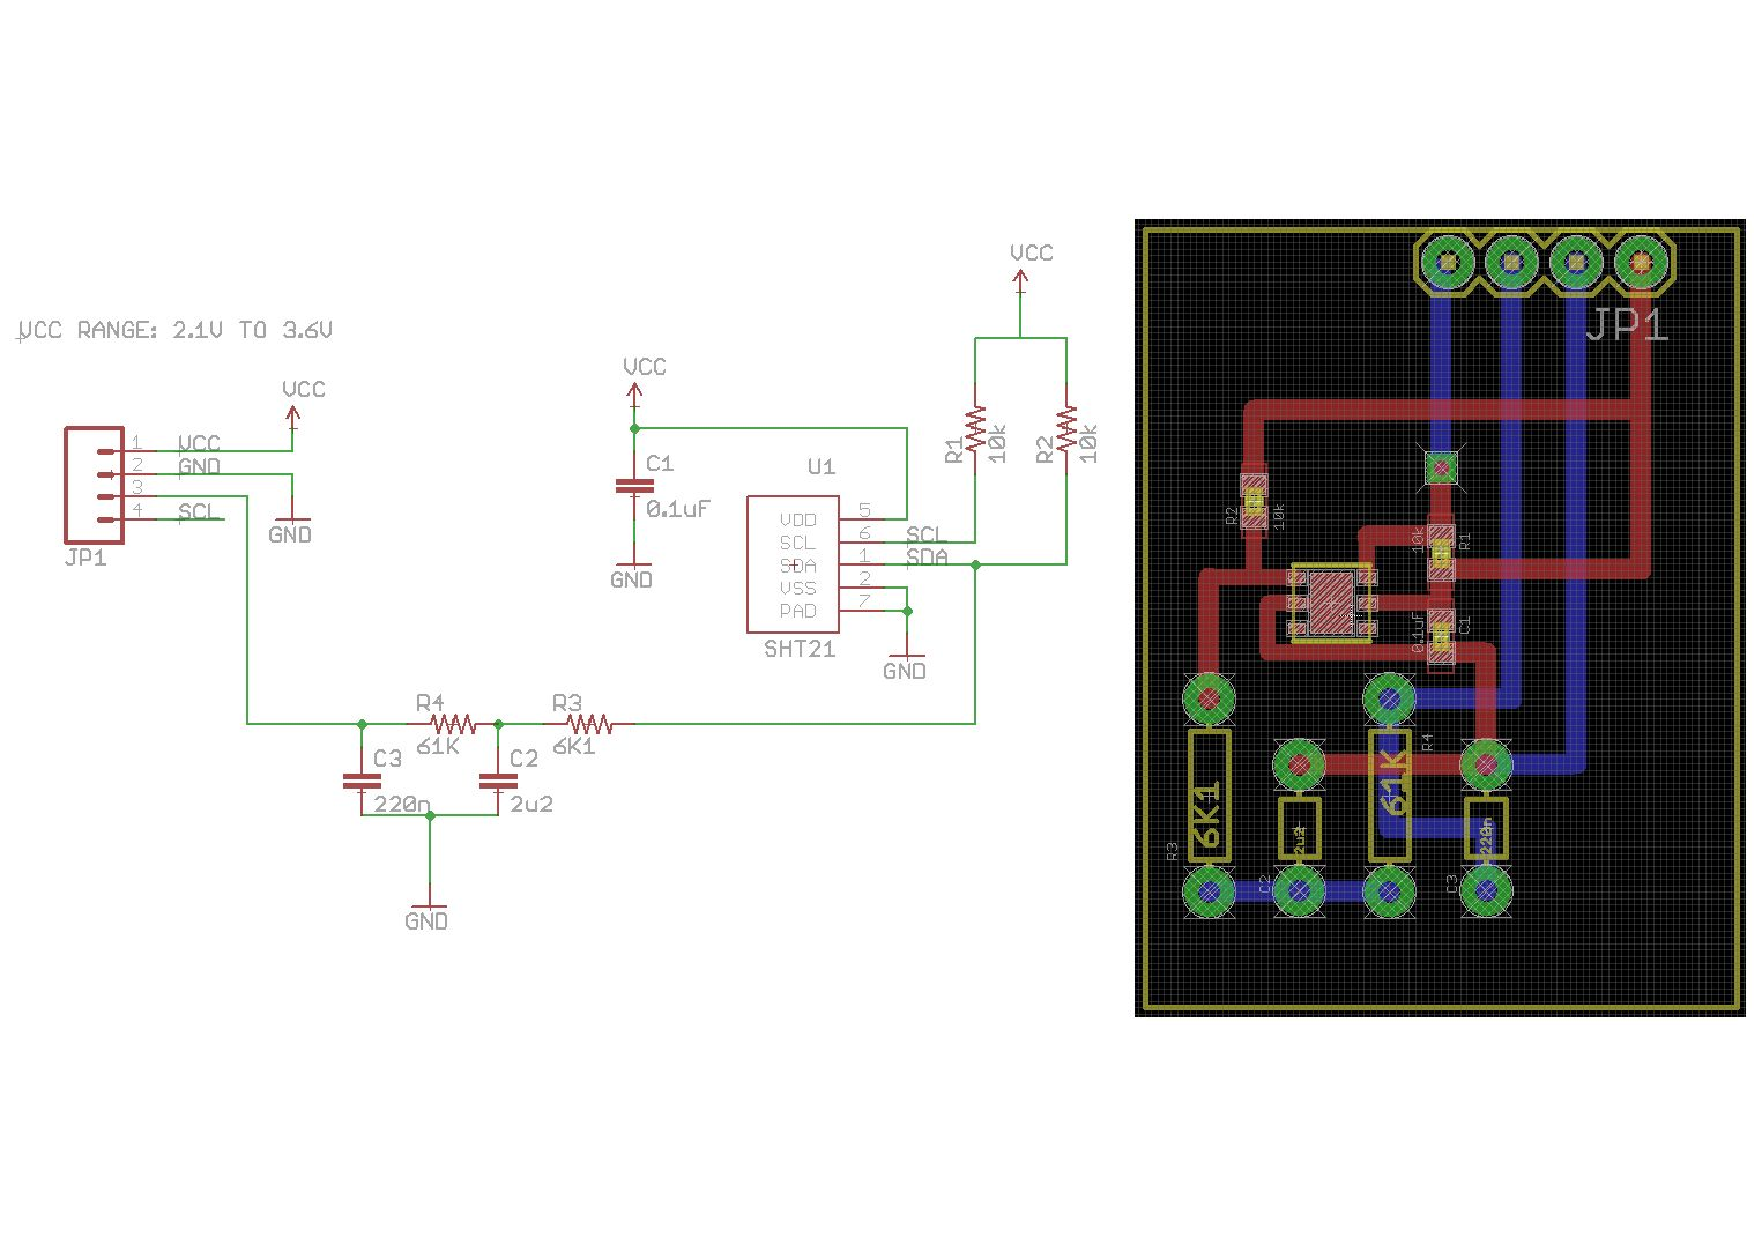
\includegraphics[width=\textwidth]{filer/implementering/SHT21P-pcb-sch}}
\caption{Schematic og layout af SHT21P kredsl\o{}b}
\label{lab:SHT21P-kredsloeb}
\end{figure}

Kredsløbet på figur \ref{lab:SHT21P-kredsloeb} blev eksporteret til gerberfiler og sendt til elektronikværkstedet som så ætsede printet og derefter monteret op.



\section{PIR-sensor (MK PO SK)}
Den PIR-sensor(HC-SR501) der er valgt til projektet har 3 ben, +POWER, OUTPUT og GND, 2 potmetre til at indstille sensitiviteten og forsinkelse samt en jumper til at indstille triggeren. Forsyningsspændingen skal ligge mellem 5V - 20V, og den har et strømforbrug på 65 mA. Forsinkelse kan justeres til mellem 0.3 - 5 min.

Output fra PIR-sensoren afgiver et TTL signal på 3.3V ved bevægelse og 0V ved stilstand.

\begin{figure}[H] \centering
{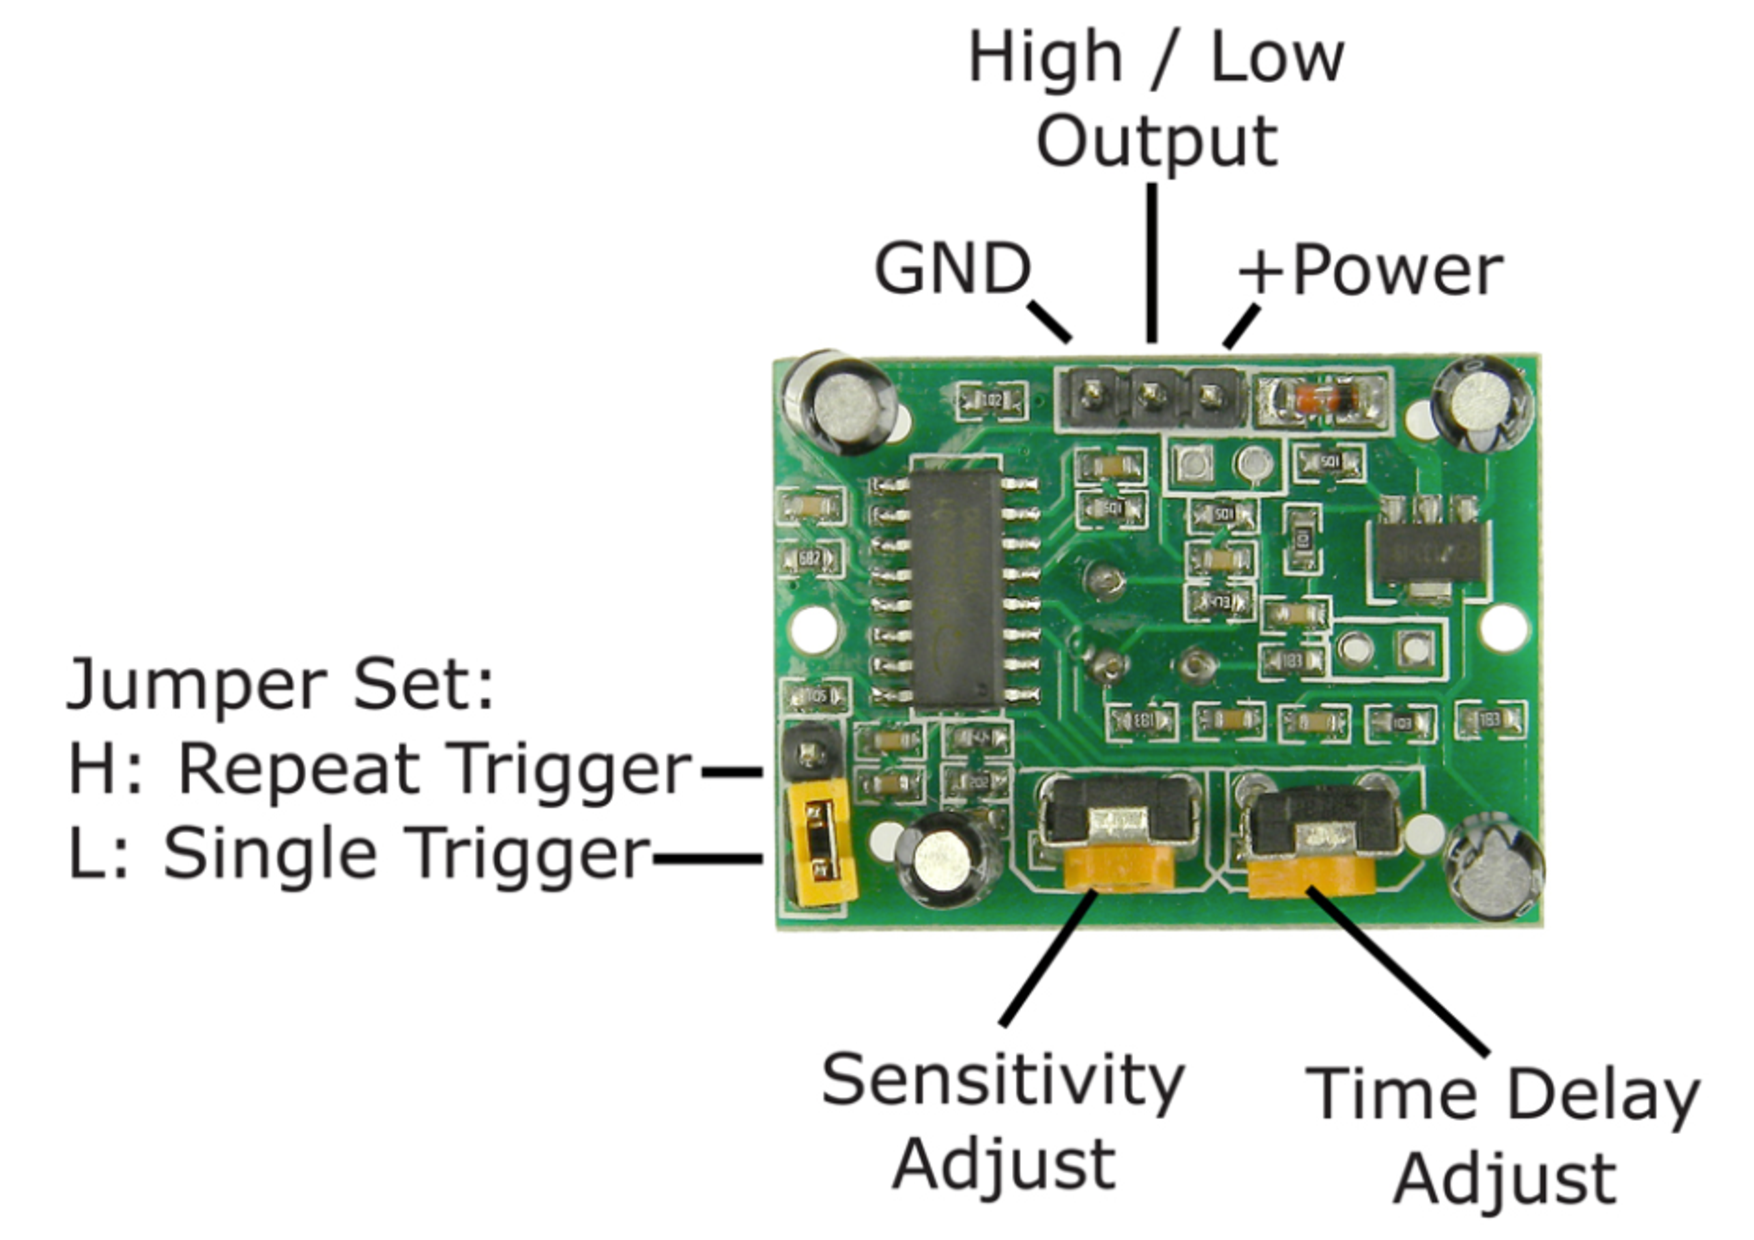
\includegraphics[width=0.5\textwidth]{filer/design/Billeder/pir_overview}}
\caption{Billede af selve printet og dets indstillingsmuligheder}
\label{lab:pir_overview}
\raggedright
\end{figure}

\subsection*{Driver}

Driveren der skal drive PIR sensoren på Enhed skal kunne registrere bevægelse via en get-metode der returnere 1(høj) ved bevægelse og 0(lav) ved stilstand.

\subsubsection*{Pseudokode}

\begin{lstlisting}[language=C]
int get_pir_status(){
Read TTL signal on P_PIR pin
Return 1 on movement and 0 on no movement
}
\end{lstlisting}

\section{Sprinkler-pumpe system (MK PO SK)}
Sprinkler-pumpe systemet består af en Hunter PS Pop-up sprinkler og en Alpha 2 pumpe fra Grundfoss, disse forbindes med passende slanger og fittings. For at styre sprinkleren, skal Alpha 2 pumpen kunne tændes og afbrydes. Dette gøres via et 230V/5V relæ. Dette relæ styres via én pin Enheden. 





\subsection{230V/5V relæ}

For at 230V/5V relæet kan blive en realitet, er det pålagt, at dette bygges i en lukket kasse og godkendes af en elektronikværksteds-ansvarlig. Kassen som bygges har et 230Vac apparatstik ind og et 230Vac stikkontakt ud. For at skabe forbindelse/afbrydelse af denne 230Vac strøm benyttes et relæ, dette relæ styrers af 5V. Når 5V  tilføjes relæets spole, klikker relæet og der skabes gennemgang fra apparatstik til stikkontakt. Dette lukkede kredsløb bygges som sagt ind i en lukke kasse med gennemsigtigt låg. Relæet der benyttes er et Finder 40.52s Figuren \ref{lab:RELAY} viser kredsløbet for dette lukkede kredsløb.

\begin{figure}[H] \centering
{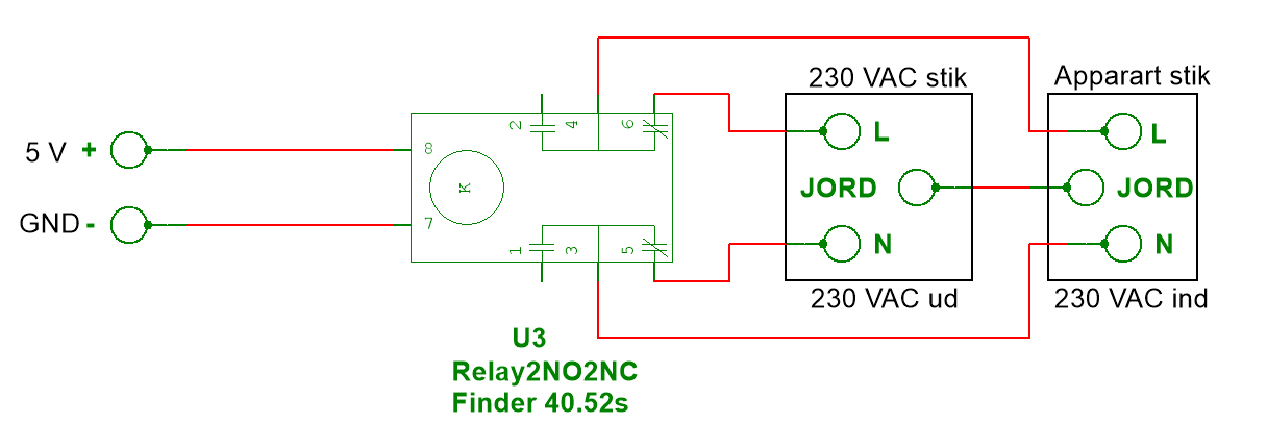
\includegraphics[width=\textwidth]{filer/design/Billeder/230VAC_KREDS}}
\caption{230V/5V relæ}
\label{lab:RELAY}
\raggedright
\end{figure}

\subsection{Alpha 2 pumpen}

Alpha 2 pumpen skal blot tilsluttes 230Vac + jord. Der medfølger et special stik til selve pumpen, dette forbindes til en 230V stikprop, med 3-ledet kabel (Leder, Nul og Jord) . Stikproppen kan nu sættes i 230V/5V relæets 230V stikkontakt.

\begin{figure}[H] \centering
{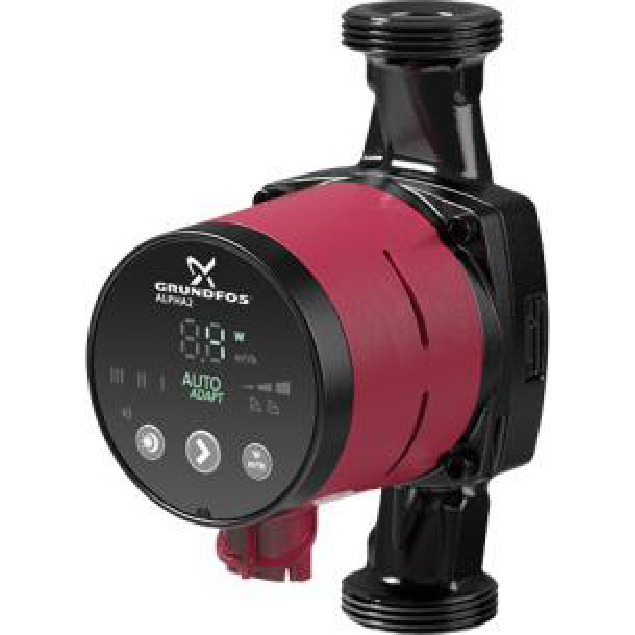
\includegraphics[width=0.4\textwidth]{filer/design/Billeder/Alpha2}}
\caption{Alpha2 Cirkulationspumpe fra Grundfoss}
\label{lab:Alpha2}
\raggedright
\end{figure} 

\subsection{Relæ styring}

I følge databladet for Finder 40.52s (figur \ref{lab:finder4052s}), kræver relæet 100mA ved 5V forsyning, som databladet

\begin{figure}[H] \centering
{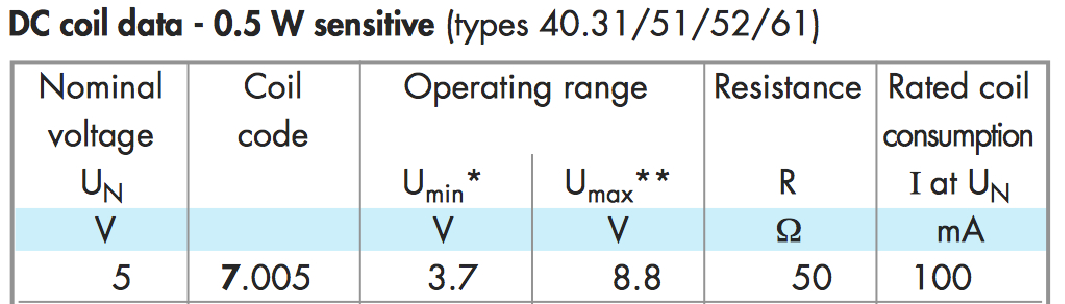
\includegraphics[width=0.7\textwidth]{filer/design/Billeder/finder4052s}}
\caption{Datablad for Finder 40.52s - 100mA}
\label{lab:finder4052s}
\raggedright
\end{figure} 

PSoC'ens udgang giver hverken strøm eller spænding nok til at trække relæet. PSoC'en afgiver 3,3V og relæet kræver 5V. For at opnå dette benyttes en transistor til styringen af relæet. Relæet kræver 5V og 100mA, derfor skal transistoren opfylde dette krav, det gør BC517 den kan leverer 500 mA. \newline

R1(Ibase) modstanden er indsat for at begrænse den strøm der går til transistorens base ben, ifølge databladet for transistoren må Ibase strømmen max være 100 mA. Spændingen ved PSoC'en er 3,3V og spændingen ved transistoren base ben er 1,4V, det giver en spænding på 1,8V over modstanden. Modstanden er beregnet udfra ohmslov og der er valgt en modstand på 18 kohm, der begrænser strømmen til 0,1 mA. Strømforstærkningen er faktisk 30000 gange i transistoren, så en strøm på 3 uA burde være nok, men der er taget et valg om at strømmen skal være 0,1 mA. Hvis modstanden blev alt for stor ville relæet tage længere tid om at trække. Databladet for BC517 har oplyst et spændingsfald på 1V i mættet tilstand det vil efterlade 4 V til relæet hvilket er nok. Dioden er indsat for at beskytte transistoren.

\begin{equation}
Ibase = \frac{1,8V}{18k\Omega} = 0,1mA
\end{equation}

\begin{figure}[H] \centering
{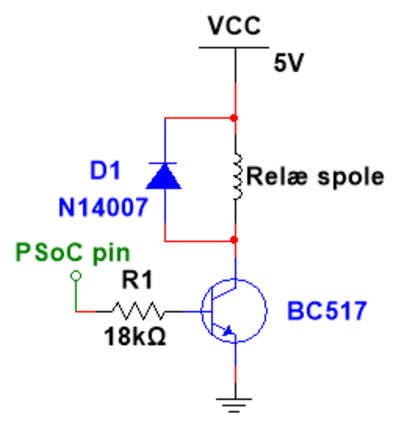
\includegraphics[width=0.3\textwidth]{filer/design/Billeder/BC517}}
\caption{BC517 opsætning}
\label{lab:BC517}
\raggedright
\end{figure} 

Når PSoC'ens pin til BC517 transistoren går høj (3,3V), så skabes der forbindelse mellem collector og emittier på transistoren, herved er der 5V over relæets spole og relæets kontaktsæt klikker herved. 

\subsection{Driver}

Driveren der skal håndtere Sprinkler-pumpe systemet, skal kunne aktivere/deaktivere det forudbestemte sprinklerrelæ. Metoden modtager en adresse parameter samt en on/off parameter. Herefter sætter metoden en af den forudbestemte pin på Enheden høj/lav (3.3V/0V). Herefter søger relæstyringen og 230V/5V relæet for hhv. tænde/slukke for sprinkleren. 


\subsubsection*{Pseudokode}

\begin{lstlisting}[language=C]
void controlSprinkler(int address, bool on_off){
Manage Sprinkler address
Activate/deactivate corresponding Sprinkler
}
\end{lstlisting}





 

\section{Strømforsyning- og tilslutningsprint (MK PO SK)}
\subsection{Strømforsyning}

For at frigøre sig fra laboratoriets strømforsyninger udarbejdes egen strømforsyning. Vha. en 230 VAC / 12 VDC switch-mode-konverter og egnede spændings-regulatorer designes en strømforsyning til netop dette projekt. Masteren (Devkit8000) har sin egen strømforsyning og denne ændres ikke. Enheden (PSoC4) skal forsynes med 5VDC via USB. Relæstyringen skal forsynes med 5VDC. PIR sensoren skal forsynes med 5-20 VDC. Temperatur/fugt sensoren skal forsynes med 3,3 VDC. 

230 VAC / 12 VDC switch-mode-konverteren er fra en gammel computer. Denne kan give 2 ampere og er forsynet med et DC stik (12V ) og en stikprop (230 VAC). Denne transformer bruges som den er. 

For at regulere fra de 12 V til 5 V benyttes en spændingsregulator. LM7805 er beregnet netop til dette formål. Ud fra figur \ref{lab:LM7805} ses forbindelsen af LM7805'ern. Databladet foreskriver også at regulatoren kan give et output på max 1 A med korrekt køling.  
\newline
Uden køling må der max afsættes 1 W i serieregulatoren, da dens arbejdstemperatur ved 1 W ligger på 100$^{\circ}$C.  I formel \ref{eq:effekt_1} er der foretaget en effektberegning på LM7805. Spændingsforskellen imellem $V_{DC}$ og $V_{OUT}$ ganges på det samlede strømforbrug. Strømforbruget er fundet i samtlige datablade for hver komponent, de kan findes på CD'en. Effektudregningen i \ref{eq:effekt_2} viser at ved fuld belastning er det nødvendigt at køle. Det er der gjort med køleplader. 

\begin{equation} 
P = (V_{DC}-V_{out})*I_{samlet} 
\label{eq:effekt_1}
\end{equation}
\begin{equation} 
P = (12V - 5V)*0,6665 A= 4,7 W 
\label{eq:effekt_2}
\end{equation}

\begin{figure}[H] \centering
{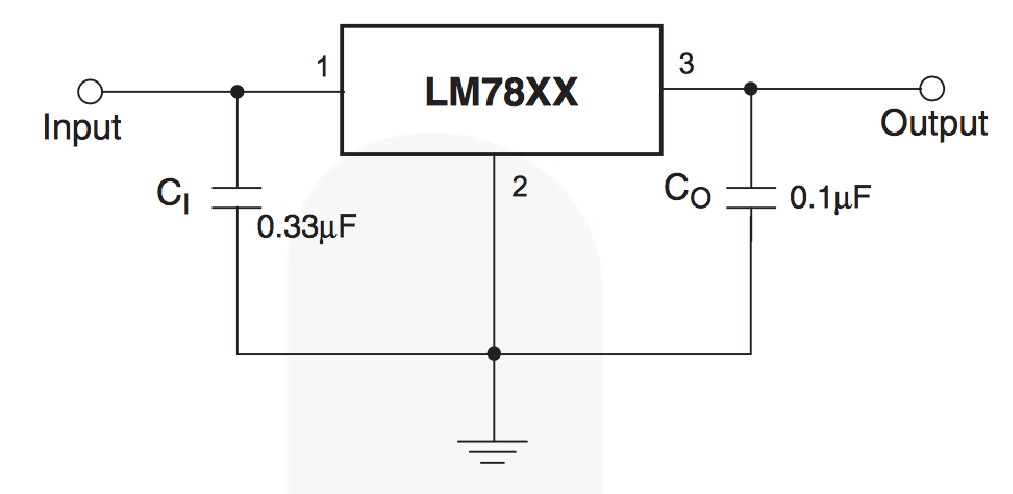
\includegraphics[width=\textwidth]{filer/design/Billeder/LM7805_DATASHEET}}
\caption{Forbindelse af LM7805 - Side 18/24 LM7805.pdf}
\label{lab:LM7805}
\raggedright
\end{figure}

Spændingsregulatoren LM7805 er opbygget i Multisim se figur \ref{lab:LM7805_SIMULERING}, sammen med 12 VDC forsyningen. Kredløbet er simuleret og dette viser at outputtet er de ønskede 5 V.

\begin{figure}[H] \centering
{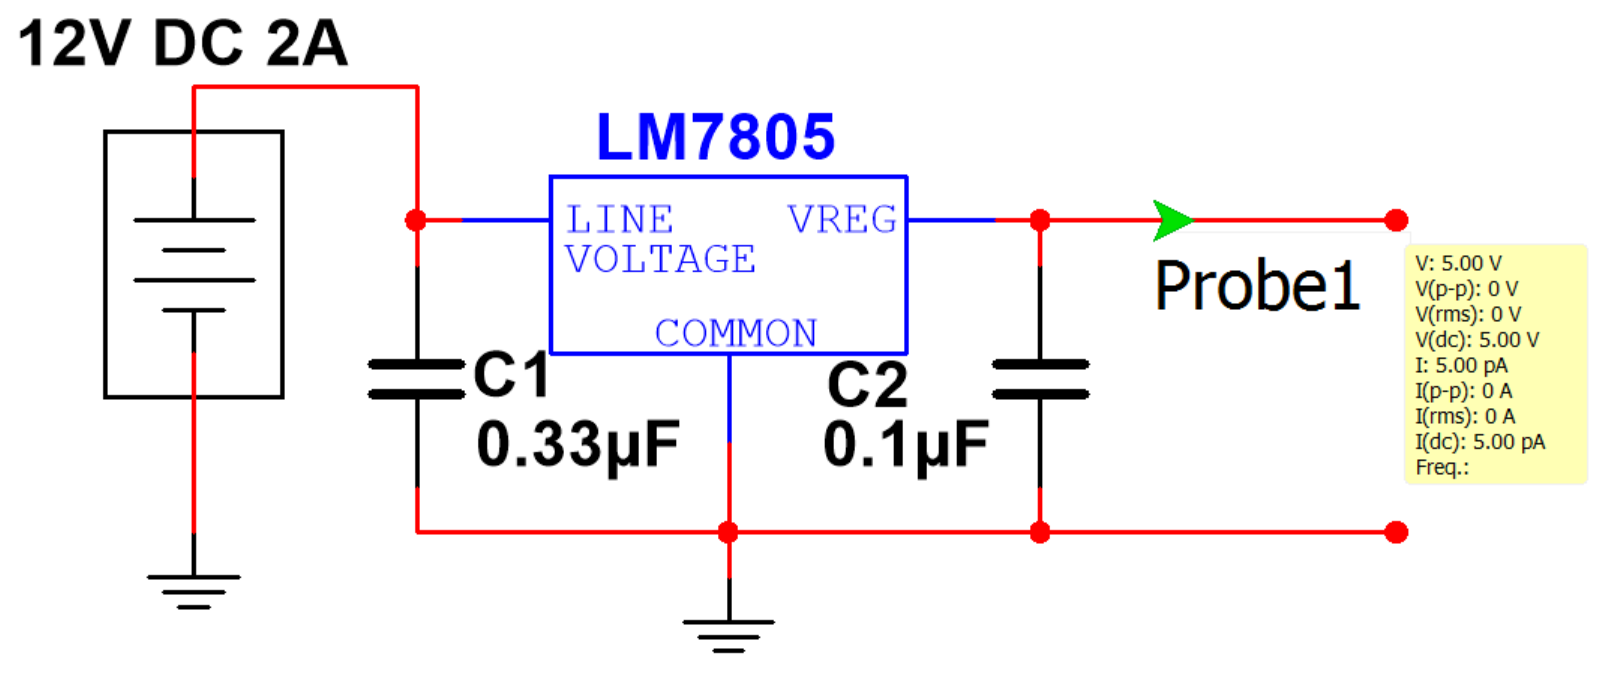
\includegraphics[width=\textwidth]{filer/design/Billeder/LM7805_SIMULATION}}
\caption{LM7805 Simulering}
\label{lab:LM7805_SIMULERING}
\raggedright
\end{figure}


For at opnå 3,3 V benyttes en justerbar spændingsregulator LM317. Denne regulator kan levere 1,2 V - 33 V 3A. Det er fugt- og temperatursensoren der skal forsynes med 3,3 V / 180 uA, det er LM317'erns opgave. 

LM317 er slået op på iPad appen "Electronic Toolbox", vha. denne gives hvordan opsætningen af denne skal være for at opnå 3,3 V 
 
\begin{figure}[H] \centering
{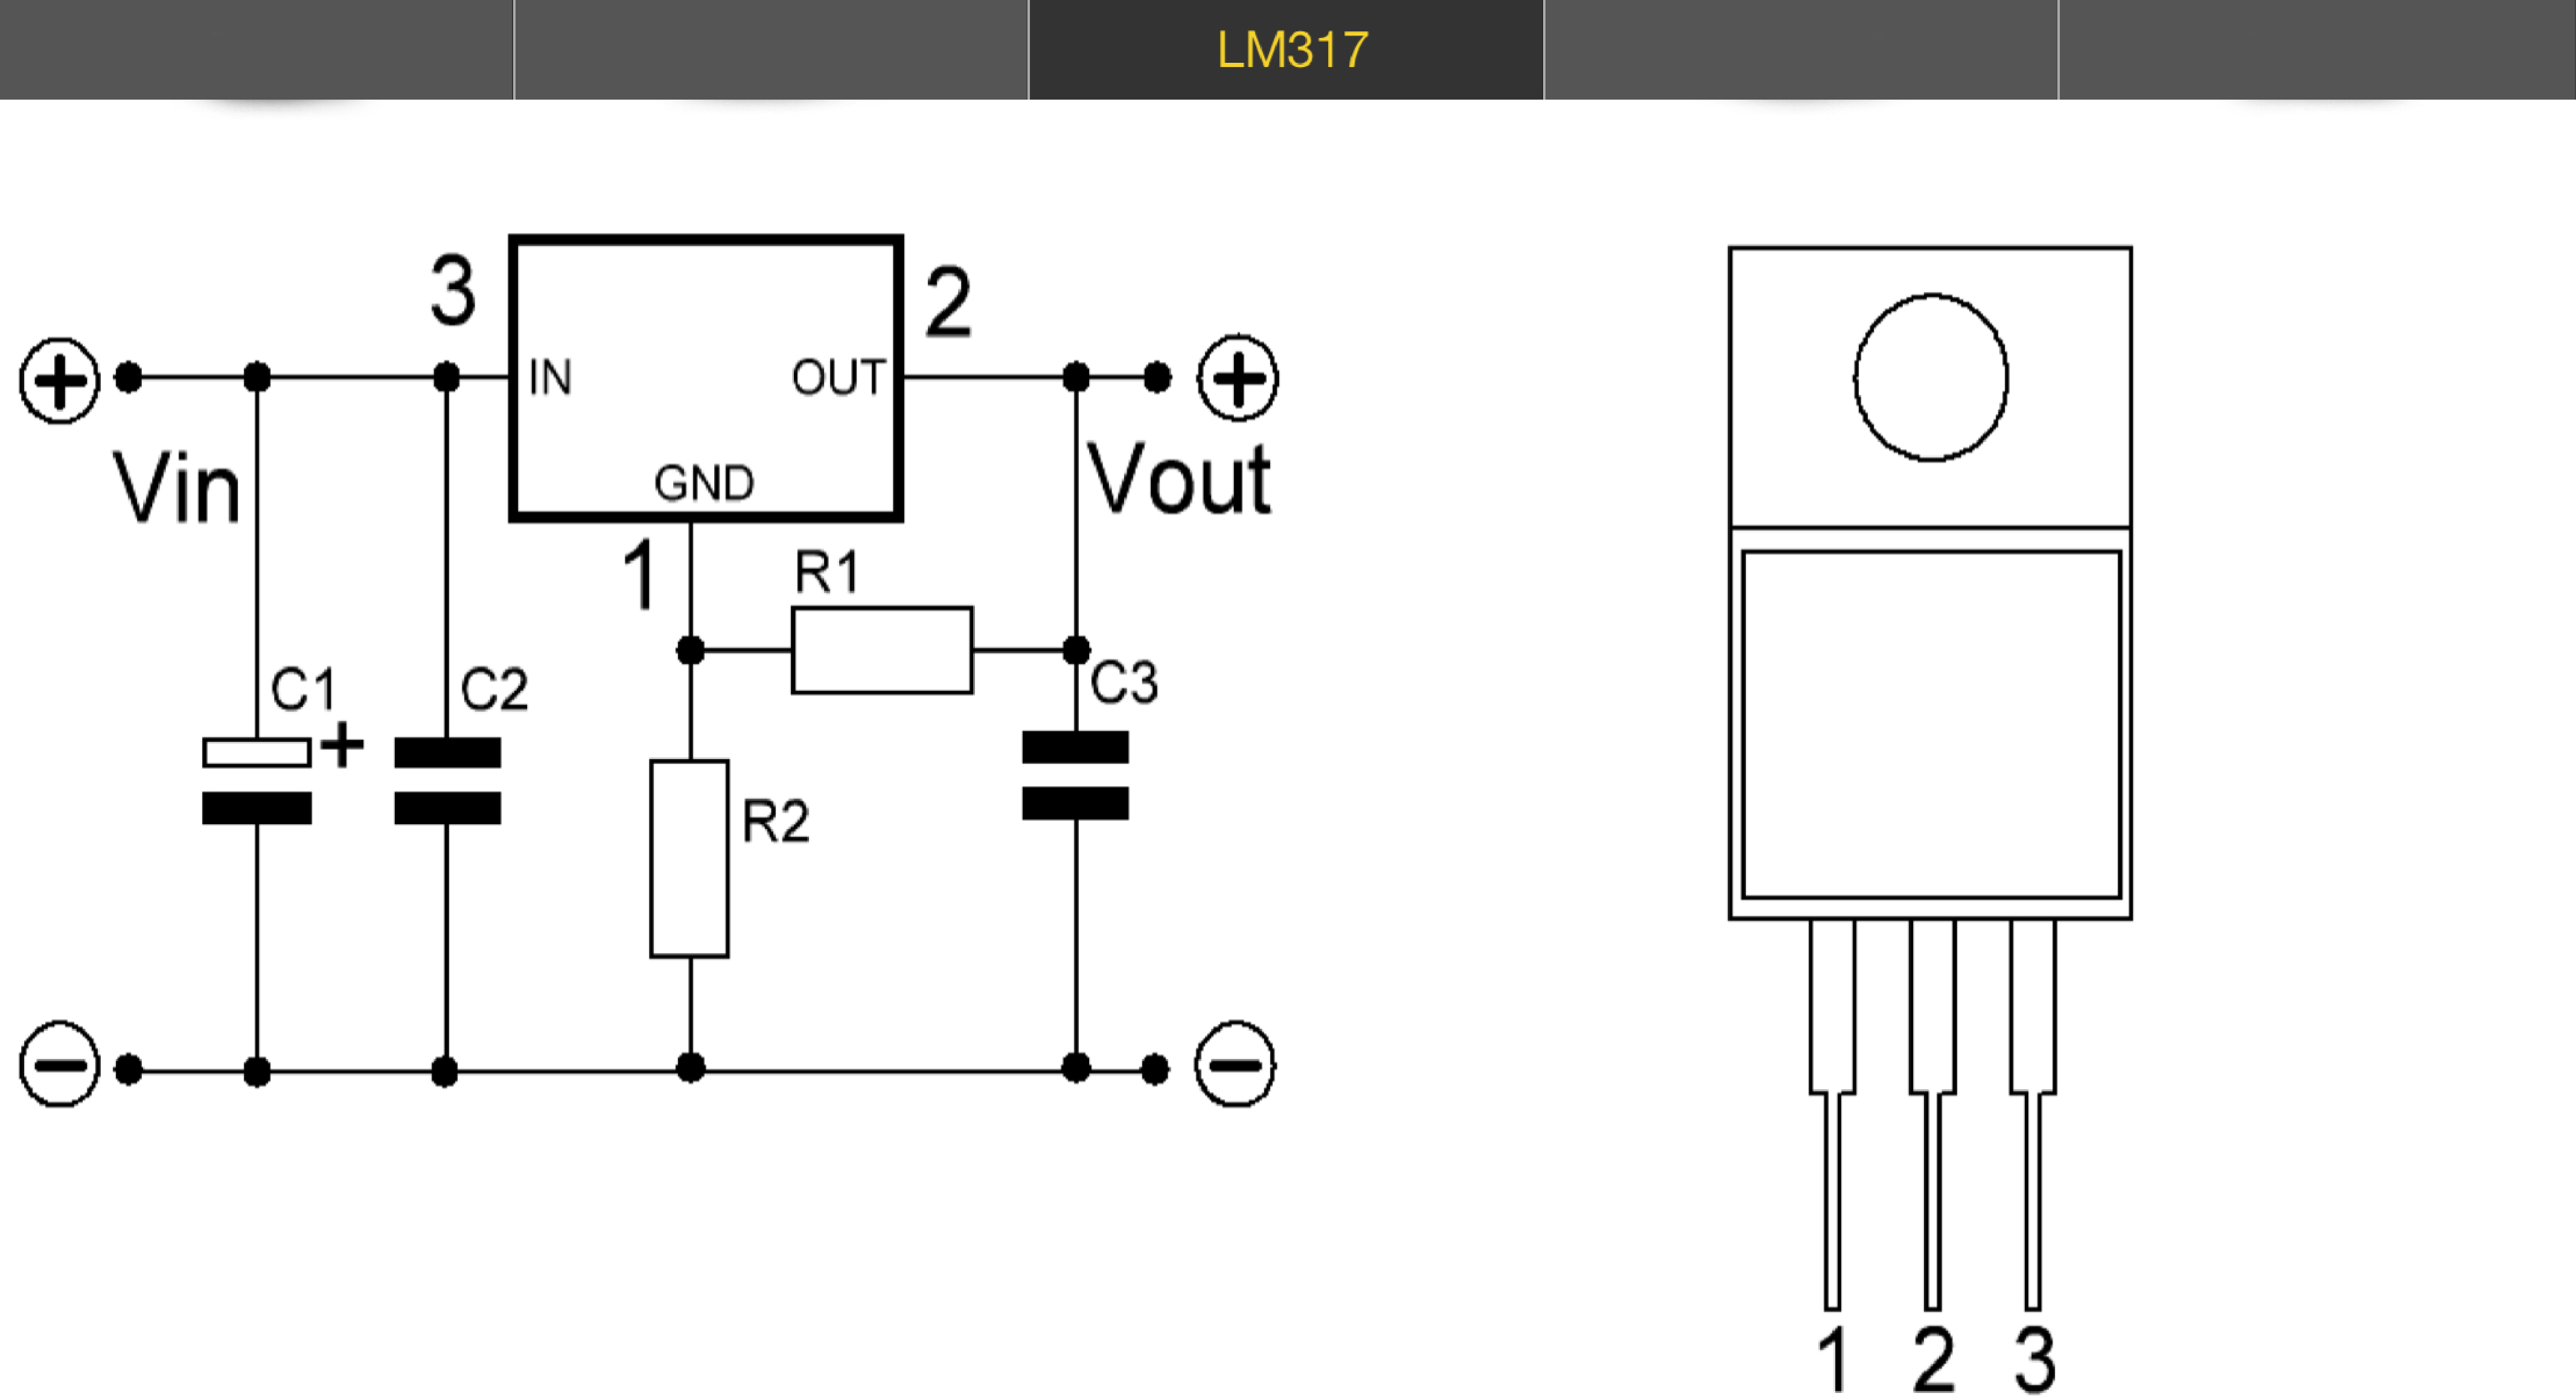
\includegraphics[width=\textwidth]{filer/design/Billeder/LM317}}
\caption{Kredsløb for LM137}
\label{lab:LM317}
\raggedright
\end{figure}

Figur \ref{lab:LM317_calc} viser hvorledes appen beregner en værdi for modstanden R2, når Vout er sat til 3,3 V og modstanden R1 anbefales til 240 ohm. I følge appens beregning skal R2 være 393,6 ohm.

\begin{figure}[H] \centering
{\includegraphics[width=\textwidth]{filer/design/Billeder/LM317_calc}}
\caption{Kredsløb for LM137}
\label{lab:LM317_calc}
\raggedright
\end{figure}

Det er muligt at beregne udgangsspændingen ud fra følgende formel \ref{eq:LM314_1} som er oplyst i databladet for LM317 og i Analogteknik\footnote{Analogteknik, Tore Skogberg, 2014, afsnit 6.8 Serieregulator, s. 259, IHA Aarhus universitet.}. Strømmen $I_Q$ er strømmen der løber fra ben 1, den er mindre end 100 uA og typisk på 50 uA, de 1,25 V er spændingen imellem udgangen og referencen. Det giver følgende resultat i formlen \ref{eq:LM314_2}. 

\begin{equation} 
V_{out} = 1,25 V*(1+\frac{R2}{R1})+I_Q*R2
\label{eq:LM314_1}
\end{equation}
\begin{equation} 
V_{out} = 1,25 V*(1+\frac{390\Omega}{240\Omega})+50uA*390\Omega = 3,3 V
\label{eq:LM314_2}
\end{equation}


I formel \ref{eq:effekt_4} er der fortaget en effektberegning på LM317. Den bliver belastet med FT-sensoren som har et strømforbrug på 180 uA, plus $I_X$ som er strømmen der løber ned i modstandene. Den er fundet ved at finde strømmen der løber i R1 vha. Ohms lov og ligge den sammen med strømmen fra ben 1 se \ref{eq:effekt_5}. Effektudregningen viser at det ikke er nødvendigt med køling, men der er dog  fortaget køling med køleplader alligevel. Det skyldes at det er altid en god ide at køle på et komponent hvis der er mulighed for det, det sikre bl.a længere levetid og berøringssikkerhed.

\begin{equation} 
I_X = \frac{1,25V}{250\Omega}+50uA = 5,2 mA  
\label{eq:effekt_5}
\end{equation} 
\begin{equation} 
P = (V_{DC}-V_{out})*(I_{FT-sensor}+I_X) 
\label{eq:effekt_3}
\end{equation}
\begin{equation} 
P = (12V - 3,3V)*(180 uA +5,2 mA)= 0,05 W 
\label{eq:effekt_4}
\end{equation}


Figur \ref{lab:LM317_SIMULERING} viser simuleringen af LM317 spændingsregulatoren. Outputtet er 3,3 V som forventet. Der simuleres med en modstand R2 på 390 ohm og ikke 393,6 ohm.

\begin{figure}[H] \centering
{\includegraphics[width=\textwidth]{filer/design/Billeder/LM317_SIMULATION}}
\caption{Simulering i Multisim ud fra Electronic Toolbox appens værdier}
\label{lab:LM317_SIMULERING}
\raggedright
\end{figure}


\subsection{Tilslutningsprint}

Tilslutningsprintet, se figur \ref{lab:PSU_connections}, sørger for at sammenkoble Enheden med de ønskede sensorer, samt at forsyne Enhed og sensorer med ønsket forsyning.

\begin{figure}[H] \centering
{\includegraphics[width=\textwidth]{filer/design/Billeder/tilslutningsprint}}
\caption{Kredsløb over samlet spændingsforsyning (3,3 V og 5 V) og tilslutninger til PSoC4}
\label{lab:PSU_connections}
\raggedright
\end{figure}



\section{SPI (MK PO SK)}
Serial Parrallel Interface (SPI) er en måde at lave hurtig seriel dataudveksling på. SPI er udviklet af Motorola og fungerer ved at man
har, som regel, en enkelt master enhed der styrer flere slave enheder. Ved SPI er der er ingen fejl-check men adressering af flere ender kan dog være 
HW krævende. I EasyWater8000 projektet er der SPI kommunikation imellem Master(devkit8000)
og Enhed(PSoC), det giver muligheden for at overføre flere data på samme tid imellem disse to.

\begin{figure}[H] \centering
{\includegraphics[width=\textwidth]{filer/design/Billeder/SPI_MASTER_SLAVE}}
\caption{SPI}
\label{lab:SPI}
\raggedright
\end{figure}

På figur \ref{lab:SPI} ses en typisk opkobling imellem Master og Slave, det kræver 4 tråde.
\begin{itemize}
 	\item SS står for "Slave select".
 	\item MISO står for "Master in slave out".
 	\item MOSI står for "Master out slave in". 
	\item SCLK står for "Serial clock" 
\end{itemize}

SPI kommunikation er baseret på skifteregister princippet, som ses på figur \ref{lab:SPI_REGISTER}. Der vælges hvilken slave der 
ønskes at skrives til ved slave select(SS), derefter shiftes et 8-bit register 1 bit ad gangen. Serial clock er den clock der sørger for at
shiftningen af bits sker korrekt, clockfrekvensen må ikke overstige grænsen for hvad enhederne kan håndtere.

\begin{figure}[H] \centering
{\includegraphics[width=\textwidth]{filer/design/Billeder/SPI_REGISTER}}
\caption{SPI register}
\label{lab:SPI_REGISTER}
\raggedright
\end{figure}  

En oftes anvendt kommunikation mellem master og slave foregår ved at master sætter SS til 0. Den fortæller nu til slaven at den er klar til 
dataoverførelse. Nu sender masteren en bit over til slaven og påbegynder en full duplex data transmission, samtidigt sender slaven en bit over
til masteren. Denne process fortsætter indtil masteren har sendt alle sine bits, derefter stopper masteren med at toggle på clocken og slave 
enheder bliver frigivet.

\subsection{Driver}



\subsubsection*{Pseudokode}

\begin{lstlisting}[language=C]

}
\end{lstlisting}

\section{Hardwareforbindelser (HW)}
\begin{table}[H]
\subsection{Enhed (HW)}
Her beskrives hvor mange og hvilke pins der skal benyttes på PSoC4 til de forskellige forbindelser.
\caption{Tabel der viser pins på PSoC4}
\begin{small}
\begin{tabular}{|p{3,5cm}|p{2cm}|p{2,9cm}|p{1,6cm}|p{2.6cm}|}
\hline

\textbf{Forbindelse}	&\textbf{Antal pins} 	&\textbf{Signalnavne} &\textbf{Pinnavne} &\textbf{Kommentar}  \\ \hline

SPI 	(P\_DK)			&4 						&MOSI				&P3[0]		&					\\\cline{3-4}
					&						&MISO				&P3[1]		&					\\\cline{3-4}
					&						&SCK					&P0[6]		&					\\\cline{3-4}
					&						&SS0					&P0[7]		&					\\\cline{3-4}
					&						&GND					&J3(GND) 	&					\\\hline
	
PIR-TTL	(P\_PIR)		&1 						&P\_PIR				&P1[1] 		&					\\\hline

Vandpumpe (VP\_01)	&4 						&SPRINKLER\_1		&P2[0]		&					\\\cline{3-4}
					&						&SPRINKLER\_2		&P2[1]		&					\\\cline{3-4}
					&						&SPRINKLER\_3		&P0[2]		&					\\\cline{3-4}
					&						&SPRINKLER\_4		&P0[3]		&					\\\hline
		
FT-sensor (P\_FT)	&5						&SELECT				&P0[0]		&Fugt/Temp.			\\\cline{3-5}
					&						&ANALOG				&P2[5]		&Analog niveau		\\\cline{3-5}
					&						&BIT0(LSB)			&P2[2]		&Adressering			\\\cline{3-5}
					&						&BIT1				&P2[3]		&Adressering			\\\cline{3-5}
					&						&BIT2(MSB)			&P2[4]		&Adressering			\\\hline			
					
Fælles GND			&1 						&GND(Forb. print)	&J2(GND) 	&Forb. print			\\\hline					
					
Enhedsadr. 			&4 						&BIT0(LSB)			&P1[2]		&					\\\cline{3-4}
					&						&BIT1				&P1[3]		&					\\\cline{3-4}
					&						&BIT2				&P1[4]		&					\\\cline{3-4}
					&						&BIT3(MSB)			&P1[5]		&					\\\hline

\end{tabular}
\end{small}
\label{table:enhed_forbindelse}
\end{table}

\begin{figure}[H]
\centering
{\includegraphics[width=0.7\textwidth]{filer/design/Billeder/psoc4_pin}}
\caption{Oversigt over fysiske pin-navne på PSoC4}
\label{lab:psoc4_pin}
\end{figure}

\newpage
\begin{table}[H]
\subsection{Master (HW)}
Her beskrives hvor mange og hvilke pins der skal benyttes på Devkit8000 til de forskellige forbindelser.
\caption{Tabel der viser pins på Devkit8000}
\begin{small}
\begin{tabular}{|p{3,5cm}|p{2cm}|p{2,9cm}|p{1,6cm}|p{2.6cm}|}
\hline

\textbf{Forbindelse}	&\textbf{Antal pins} 	&\textbf{Signalnavne} &\textbf{Pinnavne} &\textbf{Kommentar}  \\ \hline

SPI 	(P\_DK)			&5 						&MOSI				&J9.1		&					\\\cline{3-4}
					&						&MISO				&J9.2		&					\\\cline{3-4}
					&						&SCK					&J9.5		&					\\\cline{3-4}
					&						&SS0					&J9.3		&					\\\cline{3-4}					
					&						&GND					&J9.20		&					\\\hline

\end{tabular}
\end{small}
\label{table:master_forbindelse}
\end{table}

\begin{figure}[H]
\centering
{\includegraphics[width=\textwidth]{filer/design/Billeder/devkit_j9}}
\caption{Model af tilføjelses-print og J9-stik }
\label{lab:devkit_j9}
\end{figure}

%SW
\chapter{Softwaredesign}

\section{Dataprotokol (BS)}\label{header:dataprotokol}
%% SW design: Dataprotokol

\subsubsection{Aktiver, Deaktiver og Verificer}

Aktiver og Deaktiver handler ikke på enhedsnummeret.

Ved verificering af en Enhed sendes et enhedsnummer til Enheden, som der verificeres på i forhold til Enhedens enhedsnummer.

\begin{table}[h]
	\caption{Data-formatering for verificering}
	\centering
	\begin{tabular}{|l|c|}
		\hline 
		\textbf{Byte} & \textbf{Enhedsnummer} \\ 
		\hline 
		\textbf{Indhold} & ''\verb+NN+''\\ 
		\hline 
	\end{tabular} 
	\label{table:SWProtokol-verificer}
\end{table}

\subsubsection{Send parametre}

Ved parameter indstilling skal der sendes følgende parametre til Enheden.

\begin{enumerate}
	\item Enhedsnummer (1-18)
	\item Øvre temperaturgrænse
	\item Nedre fugtighedsgrænse
\end{enumerate}

Parametrene skal sendes i ovenstående rækkefølge og resulterer altså i en kommando som vist i tabel \ref{table:SWProtokol-para}. Temperaturgrænsen er begrænset til 3 heltal og én decimal. Fugtighedsgrænsen er begrænset til 3 heltal.

\begin{table}[h]
	\caption{Data-formatering for parametre}
	\centering
	\begin{tabular}{|l|c|c|c|}
		\hline 
		\textbf{Byte} & \textbf{Enhedsnummer} & \textbf{Temperatur} & \textbf{Fugtighed} \\ 
		\hline 
		\textbf{Indhold} & ''\verb+NN+'' & ''\verb+TTT.T+'' & ''\verb+FFF+''  \\ 
		\hline 
	\end{tabular} 
	\label{table:SWProtokol-para}
\end{table}

\subsubsection{Log}

Når data flyttes mellem Master og Enhed, ifm. logning, anvendes følgende dataprotokol i mellem \textit{Application}-lagene.

Den data som skal flyttes er følgende:

\begin{enumerate}
	\item Temperatur
	\item Fugtighed
	\item Bevægelsesregistrering
	\item Påbegyndt vanding
\end{enumerate}

Systemet ved ikke på forhånd hvor meget data der skal flyttes. Derfor deles det op i tre typer. Data fra sensorene, besked om bevægelse og fejlregistreringer.
Fælles for de tre er at tidsstemplet altid sendes med.

Fra standardbiblioteket for \verb'C++' vælges datatypen \verb+vector+ som container. Dette er en dynamisk array-struktur som automatisk udvides og mindskes efter behov.
Ved at anvende \verb+vector+en med \verb+string+ som undertype er det nemt at identificerer indholdene og formaterer dem som nødvendigt. På Enheden som implementeres på en PSoC er standardbiblioteket til \verb-C++- ikke tilrådighed. Derfor implementeres bufferen på denne som et almindeligt statisk allokeret char-array. Formateringen vist her under gælder for begge platforme.

Som nævnt er der flere muligheder for ''datapakker''. I tabellerne \ref{table:SWDataprotokol-sensor}, \ref{table:SWDataprotokol-bevaegelse} og \ref{table:SWDataprotokol-error} er deres opbygninger vist.

Første streng der læses afgør hvor mange af de efterfølgende strenge som høre her til. Hvis det første der modtages er ''\verb+D+'', betyder det at der kommer information fra sensorene og der skal læses fire efterfølgende strenge.
Hvis der modtages et ''\verb+E+'' er der en fejl og én streng med fejlkoden fra enheden læses.

\begin{table}[h]
	\caption{Dataformatering ifm. sensordata}
	\centering
	\begin{tabular}{|c|c|c|c|c|}
		\hline 
		\textbf{Type} & \textbf{Temperatur} & \textbf{Fugtighed} & \textbf{Vanding} & \textbf{Bevægelse}\\ 
		\hline 
		''\verb+D+'' & ''\verb+TTT.T+'' & ''\verb+FFF+'' & ''\verb+0+'' / ''\verb+1+'' & ''\verb+0+'' / ''\verb+1+'' \\ 
		\hline 
	\end{tabular} 
	\label{table:SWDataprotokol-sensor}
\end{table}

\begin{table}[h]
	\caption{Dataformatering ifm. fejl}
	\centering
	\begin{tabular}{|c|c|}
		\hline 
		\textbf{Type} & \textbf{Fejlkode} \\ 
		\hline 
		''\verb+E+'' & ''\verb+XXX+'' \\ 
		\hline 
	\end{tabular} 
	\label{table:SWDataprotokol-error}
\end{table}

Et eksempel på strukturen af en datahentning er vist i tabel \ref{table:SWDataprotokol-eksempel}. Her kan man se, at der siden sidste udlæsning har været hentet sensordata med værdierne 14.5 grader og 20\% fugtighed, der har ikke været tændt for sprinkleren men der har været bevægelse på hullet, \verb+D014.502001+ og der har også været en fejl 13, \verb+E013+.

\begin{table}[h]
	\caption{Dataformatering ifm. log-information}
	\centering
	\begin{tabular}{|c|c|}
		\hline
		\verb+vector<string>[0]+ & \verb+[1]+ \\
		\hline 
		''\verb+D014.502001+'' & ''\verb+E013+'' \\ 
		\hline 
	\end{tabular} 
	\label{table:SWDataprotokol-eksempel}
\end{table}

\section{Applikationsmodeller (JC BS)}
Selve designet af softwaren bygger på de følgende applikationsmodeller. Her laves der sekvens- og klassediagrammer over hver del af systemet samt klassebeskrivelser hvor funktionen for de enkelte metoder beskrives.

%% SW design: Applikationsmodeller

Selve designet af softwaren bygger på de følgende applikationsmodeller. Her laves der sekvens- og klassediagrammer over hver del af systemet samt klassebeskrivelser hvor funktionen for de enkelte metoder beskrives.

\subsection{Master}
Applikationsmodeller for Master.

\begin{figure}[htbp] \centering
{\includegraphics[scale=0.8]{filer/design/a_uc1}}
\caption{Sekvensdiagram UC1}
\label{fig:Sekvensdiagram UC1}
\end{figure} 

\begin{figure}[htbp] \centering
{\includegraphics[scale=0.8]{filer/design/a_uc2}}
\caption{Sekvensdiagram UC2}
\label{fig:Sekvensdiagram UC2}
\end{figure} 

\begin{figure}[htbp] \centering
{\includegraphics[scale=0.8]{filer/design/a_uc3}}
\caption{Sekvensdiagram UC3}
\label{fig:Sekvensdiagram UC3}
\end{figure} 

\begin{figure}[htbp] \centering
{\includegraphics[scale=0.8]{filer/design/a_uc4}}
\caption{Sekvensdiagram UC4}
\label{fig:Sekvensdiagram UC4}
\end{figure} 

\begin{figure}[htbp] \centering
{\includegraphics[scale=1]{filer/design/a_uc5}}
\caption{Sekvensdiagram UC5}
\label{fig:Sekvensdiagram UC5}
\end{figure} 

\begin{figure}[htbp] \centering
{\includegraphics[scale=1]{filer/design/a_uc6}}
\caption{Sekvensdiagram UC6}
\label{fig:Sekvensdiagram UC6}
\end{figure} 

\clearpage
\begin{figure}[htbp] \centering
{\includegraphics[scale=1]{filer/design/sw_class_devkit}}
\caption{klassediagram devkit8000}
\label{fig:klassediagram devkit8000}
\end{figure} 

Efter udarbejdelsen af sekvensdiagrammer samles alle metode kald imellem klasserne til et klassediagram som ses ovenfor på \ref{fig:klassediagram devkit8000}. Efter dette klassediagram udarbejdes en klassebeskrivelse hvor der tænkes over hvilke attributer de forskellige metoder skal have for at kunne udføre deres ansvar. Det bliver så fuldt op med et endeligt statisk klassediagram som inkludere alle attributer og medlems data.


\clearpage
\subsection{Enhed}
Applikationsmodeller for Enhed.

% Klassebeskrivelser
\subsection{Klassebeskrivelser}
Her følger klassebeskrivelser for de udledte klasser fra applikationsmodellerne.

% Master
\subsubsection{Master (JC)}
%% SW design: klassebeskrivelse SPI API

\begin{figure}[htbp] \centering
{\includegraphics[scale=1.5]{filer/design/Klassediagrammer/SPI_API}}
\caption{klassediagram SPI API}
\label{fig:SPI API klassediagram}
\end{figure} 

{\centering
\textbf{SPI\_api klasse}\par
}
\textbf{Ansvar:} At være det lag imellem applications laget og device driver laget. Skal håndtere snakken med device driveren til SPI kommunikation \\

int activate( int unit ) const \\
\textbf{Parametre:} modtager en integer på følgende enhed som skal aktiveres \\
\textbf{Returværdi:} returnere en integer som er 0 hvis operationen gik godt. Ved fejl returneres en negativ integer i overenstemmelse med fejl-listen \\
\textbf{Beskrivelse:} metoden skal kunne aktivere enheden som er identificeret ved integeren den modtager. Hvis dette går godt returneres 0, ellers returneres en fejlkode i overenstemmelse med fejl-listen.\\

int deactivate( int unit ) const \\
\textbf{Parametre:}  modtager en integer på følgende enhed som skal deaktiveres\\
\textbf{Returværdi}: returnere en integer som er 0 hvis operationen gik godt. Ved fejl returneres en negativ integer i overenstemmelse med fejl-listen  \\
\textbf{Beskrivelse:} metoden skal kunne deaktivere enheden som er identificeret ved integeren den modtager. Hvis dette går godt returneres 0, ellers returneres en fejlkode i overenstemmelse med fejl-listen.\\

int verify( int unit ) const \\
\textbf{Parametre:}  modtager en integer på følgende enhed som skal verificerese\\
\textbf{Returværdi:} returnere en integer som er 0 hvis operationen gik godt. Ved fejl returneres en negativ integer i overenstemmelse med fejl-listen  \\
\textbf{Beskrivelse:} metoden skal kunne verificere om en enhed, identificeret ved integeren den modtager, er på SPI nettet. Hvis dette går godt returneres 0, ellers returneres en fejlkode i overenstemmelse med fejl-listen.\\

int config( int unit, vector<string> ) const \\
\textbf{Parametre:} modtager en integer på følgende enhed som skal konfigureres. Derudover modtager den en vector af typen string som indeholder parametrene enheden skal konfigureres med \\
\textbf{Returværdi:} returnere en integer som er 0 hvis operationen gik godt. Ved fejl returneres en negativ integer i overenstemmelse med fejl-listen  \\
\textbf{Beskrivelse:} metoden skal kunne sende konfigurations parametre ud til enheder ved hjælp af device driverne til SPI kommunikationen. Hvis dette går godt returneres 0, ellers returneres en fejlkode i overenstemmelse med fejl-listen.\\

int getLog( \& vector<string>  ) \\
\textbf{Parametre:}  modtager en referance til en vector af typen string som loggen skal lægges over i.\\
\textbf{Returværdi:} returnere en integer som er 0 hvis operationen gik godt. Ved fejl returneres en negativ integer i overenstemmelse med fejl-listen  \\
\textbf{Beskrivelse:} metoden skal kunne hente log fra alle enheder på SPI netværket og gemme dem i den modtaget vector. \\









%% SW design: klassebeskrivelse UI

\begin{figure}[htbp] \centering
{\includegraphics[scale=1.5]{filer/design/Klassediagrammer/sw_UI}}
\caption{Klasse UI}
\label{fig:UI klassediagram}
\end{figure} 

{\centering
\textbf{UI}\par
}
\textbf{Ansvar:} Håndterer alt ved den grafiske brugerflade. \

\textbf{Attributter:}
\begin{itemize}
	\item \verb+QStackedWidget winStack_+ Objekt til at holde alle vinduer i
	\item \verb+winMain winMainObj_+ Hovedmenu vindue
	\item \verb+winStatus winStatusObj_+ Vis status vindue
	\item \verb+winOnOff winOnOffObj_+ Aktiver / Deaktiver vindue
	\item \verb+winAddRemove winAddRemoveObj_+ Tilføj / fjern vindue
	\item \verb+winConfig winConfigObj_+ Konfigurer vindue
	\item \verb+winConfigPar winConfigParObj_+ Konfigurer parametre vindue
	\item \verb+winAddRemovePar winAddRemoveParObj_+ Tilføj Enheds parametre vindue
	\item \verb+winLog winLogObj_+ Vis Log vindue
	\item \verb+cStatus * cStatusPtr_+ Pointer til associeret objekt
	\item \verb+cOnOff * cOnOffPtr_+ Pointer til associeret objekt
	\item \verb+cAddRemove * cAddRemovePtr_+ Pointer til associeret objekt
	\item \verb+cConfig * cConfigPtr_+ Pointer til associeret objekt
	\item \verb+cLogView * cLogViewPtr_+ Pointer til associeret objekt
\end{itemize}

\verb+UI( )+\\
\textbf{Parametre:} Ingen \\
\textbf{Returværdi:} Ingen \\
\textbf{Beskrivelse:} Tilføjer alle \verb+win+-objekterne til stakken \verb+winStack_+. Sætter det aktive vindue til hovedmenuen \verb+winMainObj_+. Indstiller størrelsen på vinduer i stakken til at fylde hele skærmen på Devkit8000, 480x272 og sætter størrelsen på \verb+UI+ til at have samme størrelse. Til sidst opsættes den centrale widget i \verb+QMainWindow+ til stakken \verb+winStack_+.\\


\verb+int setCStatus( cStatus & )+\\
\textbf{Parametre:} Reference til associeret objekt \\
\textbf{Returværdi:} 0 ved succes ellers negativ i overenstemmelse med fejl-listen. \\
\textbf{Beskrivelse:} Sætter medlemspointer til associeret controller.\\

\verb+int setCOnOff( cOnOff & )+\\
\textbf{Parametre:} Reference til associeret objekt \\
\textbf{Returværdi:} 0 ved succes ellers negativ i overenstemmelse med fejl-listen. \\
\textbf{Beskrivelse:} Sætter medlemspointer til associeret controller.\\

\verb+int setCAddRemove( cAddRemove & )+\\
\textbf{Parametre:} Reference til associeret objekt \\
\textbf{Returværdi:} 0 ved succes ellers negativ i overenstemmelse med fejl-listen. \\
\textbf{Beskrivelse:} Sætter medlemspointer til associeret controller.\\

\verb+int setCConfig( cConfig & )+\\
\textbf{Parametre:} Reference til associeret objekt \\
\textbf{Returværdi:} 0 ved succes ellers negativ i overenstemmelse med fejl-listen. \\
\textbf{Beskrivelse:} Sætter medlemspointer til associeret controller.\\

\verb+int setCLogView( cLogView & )+\\
\textbf{Parametre:} Reference til associeret objekt \\
\textbf{Returværdi:} 0 ved succes ellers negativ i overenstemmelse med fejl-listen. \\
\textbf{Beskrivelse:} Sætter medlemspointer til associeret controller.\\

\verb+cStatus * getCStatus( ) const+\\
\textbf{Parametre:} Ingen \\
\textbf{Returværdi:} 0 ved succes ellers negativ i overenstemmelse med fejl-listen. \\
\textbf{Beskrivelse:} Returnerer pointer til associeret objekt.\\

\verb+cOnOff * getCOnOff( ) const+\\
\textbf{Parametre:} Ingen \\
\textbf{Returværdi:} 0 ved succes ellers negativ i overenstemmelse med fejl-listen. \\
\textbf{Beskrivelse:} Returnerer pointer til associeret objekt.\\

\verb+cAddRemove * getCAddRemove( ) const+\\
\textbf{Parametre:} Ingen \\
\textbf{Returværdi:} 0 ved succes ellers negativ i overenstemmelse med fejl-listen. \\
\textbf{Beskrivelse:} Returnerer pointer til associeret objekt.\\

\verb+cConfig * getCConfig( ) const+\\
\textbf{Parametre:} Ingen \\
\textbf{Returværdi:} 0 ved succes ellers negativ i overenstemmelse med fejl-listen. \\
\textbf{Beskrivelse:} Returnerer pointer til associeret objekt.\\

\verb+cLogView * getCLogView( ) const+\\
\textbf{Parametre:} Ingen \\
\textbf{Returværdi:} 0 ved succes ellers negativ i overenstemmelse med fejl-listen. \\
\textbf{Beskrivelse:} Returnerer pointer til associeret objekt.\\

\verb+winOnOff * getWinOnOff( )+\\
\textbf{Parametre:} Ingen \\
\textbf{Returværdi:} 0 ved succes ellers negativ i overenstemmelse med fejl-listen. \\
\textbf{Beskrivelse:} Returnerer pointer til associeret objekt.\\

\verb+winLog * getWinLog( )+\\
\textbf{Parametre:} Ingen \\
\textbf{Returværdi:} 0 ved succes ellers negativ i overenstemmelse med fejl-listen. \\
\textbf{Beskrivelse:} Returnerer pointer til associeret objekt.\\

\verb+winAddRemove * getWinAddRemove( )+\\
\textbf{Parametre:} Ingen \\
\textbf{Returværdi:} 0 ved succes ellers negativ i overenstemmelse med fejl-listen. \\
\textbf{Beskrivelse:} Returnerer pointer til associeret objekt.\\

\verb+winAddRemovePar * getWinAddRemovePar( )+\\
\textbf{Parametre:} Ingen \\
\textbf{Returværdi:} 0 ved succes ellers negativ i overenstemmelse med fejl-listen. \\
\textbf{Beskrivelse:} Returnerer pointer til associeret objekt.\\

\verb+winConfig * getWinConfig( )+\\
\textbf{Parametre:} Ingen \\
\textbf{Returværdi:} 0 ved succes ellers negativ i overenstemmelse med fejl-listen. \\
\textbf{Beskrivelse:} Returnerer pointer til associeret objekt.\\

\verb+winConfigPar * getWinConfigPar( )+\\
\textbf{Parametre:} Ingen \\
\textbf{Returværdi:} 0 ved succes ellers negativ i overenstemmelse med fejl-listen. \\
\textbf{Beskrivelse:} Returnerer pointer til associeret objekt.\\

\verb+winStatus * getWinStatus( )+\\
\textbf{Parametre:} Ingen \\
\textbf{Returværdi:} 0 ved succes ellers negativ i overenstemmelse med fejl-listen. \\
\textbf{Beskrivelse:} Returnerer pointer til associeret objekt.\\

\verb+int setCurrent(QWidget *)+\\
\textbf{Parametre:} Pointer til vindue som skal vises i stakken. \\
\textbf{Returværdi:} 0 ved succes ellers negativ i overenstemmelse med fejl-listen. \\
\textbf{Beskrivelse:} LADER IKKE TIL AT VÆRE IMPLEMENTERET???.\\

\verb+QWidget * getCurrent( )+\\
\textbf{Parametre:} Ingen \\
\textbf{Returværdi:} 0 ved succes ellers negativ i overenstemmelse med fejl-listen. \\
\textbf{Beskrivelse:} LADER IKKE TIL AT VÆRE IMPLEMENTERET???.\\

\verb+QStackedWidget * getStack( )+\\
\textbf{Parametre:} Ingen \\
\textbf{Returværdi:} 0 ved succes ellers negativ i overenstemmelse med fejl-listen. \\
\textbf{Beskrivelse:} Returnerer pointer til winStack-objektet.\\

\verb+int showMain( )+\\
\textbf{Parametre:} Ingen \\
\textbf{Returværdi:} 0 ved succes ellers negativ i overenstemmelse med fejl-listen. \\
\textbf{Beskrivelse:} Sætter aktive vindue i \verb+winStack_+-objektet til \verb+winMainObj_+.\\

\verb+int showStatus( )+\\
\textbf{Parametre:} Ingen \\
\textbf{Returværdi:} 0 ved succes ellers negativ i overenstemmelse med fejl-listen. \\
\textbf{Beskrivelse:} Sætter aktive vindue i \verb+winStack_+-objektet til \verb+winStatusObj_+.\\

\verb+int showOnOff( )+\\
\textbf{Parametre:} Ingen \\
\textbf{Returværdi:} 0 ved succes ellers negativ i overenstemmelse med fejl-listen. \\
\textbf{Beskrivelse:} Sætter aktive vindue i \verb+winStack_+-objektet til \verb+winOnOffObj_+.\\

\verb+int showAddRemove( )+\\
\textbf{Parametre:} Ingen \\
\textbf{Returværdi:} 0 ved succes ellers negativ i overenstemmelse med fejl-listen. \\
\textbf{Beskrivelse:} Sætter aktive vindue i \verb+winStack_+-objektet til \verb+winAddRemoveObj_+.\\

\verb+int showConfig( )+\\
\textbf{Parametre:} Ingen \\
\textbf{Returværdi:} 0 ved succes ellers negativ i overenstemmelse med fejl-listen. \\
\textbf{Beskrivelse:} Sætter aktive vindue i \verb+winStack_+-objektet til \verb+winConfigObj_+.\\

\verb+int showParam( )+\\
\textbf{Parametre:} Ingen \\
\textbf{Returværdi:} 0 ved succes ellers negativ i overenstemmelse med fejl-listen. \\
\textbf{Beskrivelse:} Sætter aktive vindue i \verb+winStack_+-objektet til \verb+winConfigParObj_+.\\

\verb+int showAddRemovePar( )+\\
\textbf{Parametre:} Ingen \\
\textbf{Returværdi:} 0 ved succes ellers negativ i overenstemmelse med fejl-listen. \\
\textbf{Beskrivelse:} Sætter aktive vindue i \verb+winStack_+-objektet til \verb+winAddRemoveParObj_+.\\

\verb+int showLog( )+\\
\textbf{Parametre:} Ingen \\
\textbf{Returværdi:} 0 ved succes ellers negativ i overenstemmelse med fejl-listen. \\
\textbf{Beskrivelse:} Sætter aktive vindue i \verb+winStack_+-objektet til \verb+winLogObj_+.\\


%% SW design: klassebeskrivelse devkit Controllers
\newpage

\begin{figure}[htbp] \centering
{\includegraphics[scale=1.5]{filer/design/Klassediagrammer/sw_addRemove}}
\caption{klassediagram addRemove}
\label{fig:addRemove klassediagram}
\end{figure} 

{\centering
\textbf{addRemove}\par
}
\textbf{Ansvar:} at styre forløbet i UC1: Tilføj / fjern enhed. \

\verb+int menuAddRemove( ) const+ \\
\textbf{Parametre:} Modtager ingen parametre \\
\textbf{Returværdi:} 0 ved succes ellers negativ i overenstemmelse med fejl-listen \\
\textbf{Beskrivelse:} Modtager information fra brugeren omkring enhed, verificere enheden over SPI netværket og gemme information i databasen..\\

\begin{figure}[htbp] \centering
{\includegraphics[scale=1.5]{filer/design/Klassediagrammer/sw_config}}
\caption{klassediagram config}
\label{fig:config klassediagram}
\end{figure} 

{\centering
\textbf{Config}\par
}
\textbf{Ansvar:} at styre forløbet i UC2: Konfig. \

\verb+int menuConfig( ) const+ \\
\textbf{Parametre:} Modtager ingen parametre \\
\textbf{Returværdi:} 0 ved succes ellers negativ i overenstemmelse med fejl-listen \\
\textbf{Beskrivelse:} Modtager information fra brugeren omkring enhed og parametre. Parametrene skrives til den pågældende enhed på SPI netværket.\\

\begin{figure}[htbp] \centering
{\includegraphics[scale=1.5]{filer/design/Klassediagrammer/sw_onOff}}
\caption{klassediagram onOff}
\label{fig:onOff klassediagram}
\end{figure} 

\newpage

{\centering
\textbf{onOff}\par
}
\textbf{Ansvar:} at styre forløbet i UC3: Aktiver / deaktiver. \

\verb+int menuOnOff( ) const+ \\
\textbf{Parametre:} Modtager ingen parametre \\
\textbf{Returværdi:} 0 ved succes ellers negativ i overenstemmelse med fejl-listen \\
\textbf{Beskrivelse:} Modtager information fra brugeren omkring hvilken enhed som ønskes aktiveret eller deaktiveret. Enheden modtager informationen over SPI netværket.\\

\begin{figure}[htbp] \centering
{\includegraphics[scale=1.5]{filer/design/Klassediagrammer/sw_loadData}}
\caption{klassediagram loadData}
\label{fig:loadData klassediagram}
\end{figure} 

{\centering
\textbf{loadData}\par
}
\textbf{Ansvar:} at styre forløbet i UC4: Databehandling . \

\verb+void getData( )+ \\
\textbf{Parametre:} Modtager ingen parametre \\
\textbf{Returværdi:} 0 ved succes ellers negativ i overenstemmelse med fejl-listen \\
\textbf{Beskrivelse:} Kaldes af en uafhængig tråd når en timer løber ud. Skal hente log-data over SPI netværket. Kontrollerer om der er nogle sensor-læsninger i mellem dataen og gemme denne i \verb+log+-objektet. Fejl gemmes ikke i \verb+log+.\\

\begin{figure}[htbp] \centering
{\includegraphics[scale=1.5]{filer/design/Klassediagrammer/sw_status}}
\caption{klassediagram status}
\label{fig:status klassediagram}
\end{figure} 

\newpage

{\centering
\textbf{status}\par
}
\textbf{Ansvar:} at styre forløbet i UC5: Tjek status. \

\verb+int menuStatus( ) const+ \\
\textbf{Parametre:} Modtager ingen parametre \\
\textbf{Returværdi:} 0 ved succes ellers negativ i overenstemmelse med fejl-listen \\
\textbf{Beskrivelse:} Henter den seneste log i hukommelsen og viser brugeren den, for den ønskede enhed.\\

\begin{figure}[htbp] \centering
{\includegraphics[scale=1.5]{filer/design/Klassediagrammer/sw_logView}}
\caption{klassediagram logView}
\label{fig:logView klassediagram}
\end{figure}

{\centering
\textbf{logView}\par
}
\textbf{Ansvar:} at styre forløbet i UC6: Udskriv log. \

\verb+int menuLog( ) const+ \\
\textbf{Parametre:} Modtager ingen parametre \\
\textbf{Returværdi:} 0 ved succes ellers negativ i overenstemmelse med fejl-listen \\
\textbf{Beskrivelse:} Henter hele loggen i hukommelsen og viser brugeren den, for den ønskede enhed.\\


%% SW design: klassebeskrivelse devkit domain klasser
\newpage

\begin{figure}[htbp] \centering
{\includegraphics[scale=1.5]{filer/design/Klassediagrammer/sw_unitDB}}
\caption{Klasse unitDB}
\label{fig:unitDB klassediagram}
\end{figure} 

{\centering
\textbf{unitDB}\par
}
\textbf{Ansvar:} Gemmer opsatte Enheder og deres parametre. \

\textbf{Attributter:}
\begin{itemize}
	\item \verb+vector< vector<string> > * unitDB_+ Dynamisk allokeret \verb+vector+ til enhedsliste.
\end{itemize}

\verb+unitDB( ) +\\
\textbf{Parametre:} Ingen.\\
\textbf{Returværdi:} Ingen. \\
\textbf{Beskrivelse:} Allokerer dynamisk en \verb+vector< vector<string> >+ til attributten \verb+unitDB_+. Indsætter 18 enheder af typen \verb+vector<string>+ med grænserne -1 for temperatur og fugtighed, og status sættes til [Deaktiv] på hhv. index 1, 2, 3. Index 0 er nummeret på enheden. \\

\verb+~unitDB( ) +\\
\textbf{Parametre:} Ingen.\\
\textbf{Returværdi:} Ingen. \\
\textbf{Beskrivelse:} Deallokerer \verb+unitDB_+. \\

\verb+int getUnits( vector< vector<string> > * ) +\\
\textbf{Parametre:} Modtager pointer til hvor enhedslisten skal gemmes.\\
\textbf{Returværdi:} 0 ved succes ellers negativ i overenstemmelse med fejl-listen. \\
\textbf{Beskrivelse:} Skriver indholdet af \verb+unitDB_+ over i den modtagne pointer. \\

\verb+int saveUnit( vector<string> ) +\\
\textbf{Parametre:} \verb+vector+ som skal gemmes \\
\textbf{Returværdi:} 0 ved succes ellers negativ i overenstemmelse med fejl-listen. \\
\textbf{Beskrivelse:} Finder enhedsnummer fra modtagne vektor og gemmer data i den pågældende plads i \verb+unitDB_+. \\

\begin{figure}[htbp] \centering
{\includegraphics[scale=1.5]{filer/design/Klassediagrammer/sw_log}}
\caption{Klasse log}
\label{fig:log klassediagram}
\end{figure} 

{\centering
\textbf{log}\par
}
\textbf{Ansvar:} Gemmer log-information fra tilkoblede Enheder. \

\textbf{Attributter:}
\begin{itemize}
	\item \verb+vector< vector<string> > * log_+ Dynamisk allokeret \verb+vector+ til loggen.
	\item \verb+vector<string> * latest_+ Dynamisk allokeret \verb+vector+ til senest loggede information.
\end{itemize}

\verb+log( ) +\\
\textbf{Parametre:} Ingen \\
\textbf{Returværdi:} Ingen\\
\textbf{Beskrivelse:} Allokerer dynamisk en \verb+vector< vector<string> >+ til \verb+log_+ og en \verb+vector<string>+ til \verb+latest_+. \\

\verb+~log( ) +\\
\textbf{Parametre:} Ingen \\
\textbf{Returværdi:} Ingen\\
\textbf{Beskrivelse:} Deallokerer \verb+log_+ og \verb+latest_+. \\

\verb+int saveLog( vector<string> ) +\\
\textbf{Parametre:} \verb+vector+ som skal gemmes. \\
\textbf{Returværdi:} 0 ved succes ellers negativ i overenstemmelse med fejl-listen. \\
\textbf{Beskrivelse:} Gemmer modtaget data ved at pushe \verb+log_+ og overskrive \verb+latest+. \\

\verb+int getLog( vector< vector<string> > * ) + \\
\textbf{Parametre:} Pointer til hvor data skal gemmes. \\
\textbf{Returværdi:} 0 ved succes ellers negativ i overenstemmelse med fejl-listen. \\
\textbf{Beskrivelse:} Skriver data fra \verb+log_+ over i modtagne pointer. \\

\verb+int getLatest( vector<string> * ) +\\
\textbf{Parametre:} Pointer til hvor data skal gemmes.  \\
\textbf{Returværdi:} 0 ved succes ellers negativ i overenstemmelse med fejl-listen. \\
\textbf{Beskrivelse:} Skriver data fra \verb+latest_+ over i modtagne pointer. \\




% Enhed
\subsubsection{Enhed (BS)}
Her følger klassebeskrivelser til Enhed. 
Bemærk at alt kode til PSoC er skrevet i \verb+C+, hvorfor det ikke er muligt at lave klasser. Beskrivelserne tager dog udgangspunkt i \verb-C++-, men skal fortolkes iht. beskrivelsen i \textit{UML-Light}\footnote{T-133 UML-Light af Finn Overgaard Hansen. Benyttet i forbindelse med faget I1OPRG (Objektorienteret PRoGrammering) på 1. semester.} 

%% SW design: PSoC Controllers

\begin{figure}[htbp] \centering
{\includegraphics[scale=1.3]{filer/design/Klassediagrammer/sw_psoc_addRemove}}
\caption{Klasse addRemove}
\label{fig:sw_psoc_class_addremove}
\end{figure} 

{\centering
\textbf{addRemove}\par
}
\textbf{Ansvar:} Kontrollerer hændelsesforløbet ifm. usecase 1. \

\verb+int verify( ) const +\\
\textbf{Parametre:} Ingen \\
\textbf{Returværdi:} 0 ved succes ellers negativ i overenstemmelse med fejl-listen. \\
\textbf{Beskrivelse:} Returnerer kun 0. Bruges til at verificerer kommunikation mellem Master og Enhed.\\

\begin{figure}[htbp] \centering
{\includegraphics[scale=1.3]{filer/design/Klassediagrammer/sw_psoc_config}}
\caption{Klasse config}
\label{fig:sw_psoc_class_config}
\end{figure} 

{\centering
\textbf{config}\par
}
\textbf{Ansvar:} Kontrollerer hændelsesforløbet ifm. usecase 2. \

\verb+int config( float & temp const, float & humidity const )+ \\
\textbf{Parametre:} To referencer til hhv. temperatur og fugtighedsgrænser \\
\textbf{Returværdi:} 0 ved succes ellers negativ i overenstemmelse med fejl-listen. \\
\textbf{Beskrivelse:} Skal gemme parametre i et objekt af typen parameters.\\

\begin{figure}[htbp] \centering
{\includegraphics[scale=1.3]{filer/design/Klassediagrammer/sw_psoc_onOff}}
\caption{Klasse onOff}
\label{fig:sw_psoc_class_onOff}
\end{figure} 

{\centering
\textbf{onOff}\par
}
\textbf{Ansvar:} Kontrollerer hændelsesforløbet ifm. usecase 3. \

\verb+int turnOnOff( bool onOff const )+ \\
\textbf{Parametre:} En \verb+bool+ som angiver on = true, off = false \\
\textbf{Returværdi:} 0 ved succes ellers negativ i overenstemmelse med fejl-listen. \\
\textbf{Beskrivelse:} Skal sætte flaget \verb+active_+ i \verb+parameters+-objektet ud fra den modtagende parameter.\\

\begin{figure}[htbp] \centering
{\includegraphics[scale=1.3]{filer/design/Klassediagrammer/sw_psoc_loadData}}
\caption{Klasse loadData}
\label{fig:sw_psoc_class_loadData}
\end{figure} 

{\centering
\textbf{loadData}\par
}
\textbf{Ansvar:} Kontrollerer hændelsesforløbet ifm. usecase 4. \

\verb+int getBuffer( vector<string> & buf )+ \\
\textbf{Parametre:} En reference til en skrivbar buffer \\
\textbf{Returværdi:} 0 ved succes ellers negativ i overenstemmelse med fejl-listen. \\
\textbf{Beskrivelse:} Skal hente data fra \verb+buffer+-objektet og gemme det i parametren buf.\\

\verb+int movementDetekt( )+ \\
\textbf{Parametre:} Ingen. \\
\textbf{Returværdi:} 0 ved succes ellers negativ i overenstemmelse med fejl-listen. \\
\textbf{Beskrivelse:} Skal deaktiverer vanding ved at sætte \verb+active_+-flaget i \verb+parameters+-objektet til 0. Skal også starte en timer som ved udløbet skal aktiverer vandingen igen efter 30 minutter.\\
%% SW design: PSoC Domain

\begin{figure}[htbp] \centering
{\includegraphics[scale=1.3]{filer/design/Klassediagrammer/sw_psoc_parameters}}
\caption{Klasse parameters}
\label{fig:sw_psoc_class_parameters}
\end{figure} 

{\centering
\textbf{parameters}\par
}
\textbf{Ansvar:} Gemme information om grænseværdier mv. til det autonome vandingssystem. \

\verb+int setTemp( float temp const ) +\\
\textbf{Parametre:} temperatur. \\
\textbf{Returværdi:} 0 ved succes ellers negativ i overenstemmelse med fejl-listen. \\
\textbf{Beskrivelse:} Gemmer modtagne temperatur i medlemsdata \verb+temperature_+. \\

\verb+int getTemp( float * temp )+ \\
\textbf{Parametre:} Pointer til at gemme temperatur i. \\
\textbf{Returværdi:} 0 ved succes ellers negativ i overenstemmelse med fejl-listen. \\
\textbf{Beskrivelse:} Returnerer medlem \verb+temperature_+ i reference. \\

\verb+int setHumi( float humi const )+ \\
\textbf{Parametre:} humidity. \\
\textbf{Returværdi:} 0 ved succes ellers negativ i overenstemmelse med fejl-listen. \\
\textbf{Beskrivelse:} Gemmer modtagne humidity i medlemsdata \verb+humidity_+. \\

\verb+int getHumi( float * humi )+ \\
\textbf{Parametre:} Pointer til at gemme humidity i. \\
\textbf{Returværdi:} 0 ved succes ellers negativ i overenstemmelse med fejl-listen. \\
\textbf{Beskrivelse:} Returnerer medlem \verb+humidity_+ i reference. \\

\verb+int setActive( unsigned char const )+ \\
\textbf{Parametre:} 1 = aktiv, 0 = inaktiv. \\
\textbf{Returværdi:} 0 ved succes ellers negativ i overenstemmelse med fejl-listen. \\
\textbf{Beskrivelse:} Gemmer modtagne char i medlemsdata \verb+active_+. \\

\verb+int getActive( unsigned char * )+ \\
\textbf{Parametre:} Pointer til at gemme unsigned char i. \\
\textbf{Returværdi:} 0 ved succes ellers negativ i overenstemmelse med fejl-listen. \\
\textbf{Beskrivelse:} Returnerer medlem \verb+active_+ i pointer. \\


\begin{figure}[htbp] \centering
{\includegraphics[scale=1.3]{filer/design/Klassediagrammer/sw_psoc_buffer}}
\caption{Klasse buffer}
\label{fig:sw_psoc_class_buffer}
\end{figure} 

{\centering
\textbf{buffer}\par
}
\textbf{Ansvar:} Holde data fra sensorerne indtil de udlæses af Master \

\verb+buffer( )+ \\
\textbf{Parametre:} Ingen. \\
\textbf{Returværdi:} Ingen. \\
\textbf{Beskrivelse:} Skal initialisere \verb+char+ array \verb+buffer_+ med plads til én datamåling og 10 fejl iht. dataprotokol. \\

\verb+int saveData( char * buf const, unsigned int len const )+ \\
\textbf{Parametre:} Pointer til buffer med len data. \\
\textbf{Returværdi:} 0 ved succes ellers negativ i overenstemmelse med fejl-listen. \\
\textbf{Beskrivelse:} Skal gemme modtaget data i \verb+buffer_+-medlemmet og flytte \verb+cursor_+ antallet af karakterer frem.\\

\verb+int getData( char * buf, unsigned int len )+ \\
\textbf{Parametre:} Pointer til char array til data. \\
\textbf{Returværdi:} 0 ved succes ellers negativ i overenstemmelse med fejl-listen. \\
\textbf{Beskrivelse:} Skal returnerer data fra \verb+buffer_+ i pointer og nulstille \verb+cursor_+-medlemmet.\\
%% SW design: PSoC Boundary

\begin{figure}[htbp] \centering
{\includegraphics[scale=1.3]{filer/design/Klassediagrammer/sw_psoc_SPIhandler}}
\caption{Klasse spi}
\label{fig:sw_psoc_class_spi}
\end{figure} 

{\centering
\textbf{spi}\par
}
\textbf{Ansvar:} Håndterer kommunikation i mellem Master og Enhed. \

\textbf{Attributter:}
\begin{itemize}
	\item \verb+char spiBuffer[]+ Bruges til modtagede SPI kommandoer fra Master
	\item \verb+char spiTxBuffer[]+ Bruges til afsendelse af SPI kommandoer til Master
	\item \verb+char unitNo+ Enheds nummer til verificering
	\item \verb+int spiCounter+ Tæller til antallet af modtagne data-stykker
	\item \verb+int spiReadCounter+ Tæller til antallet af afsendte data-stykker
	\item \verb+unsigned int len+ Længde til afsendelse af log-data
	\item \verb+char tempBuffer[]+ Midlertidig buffer til konfigurering af parametre
	\item \verb+char humiBuffer[]+ Midlertidig buffer til konfigurering af parametre
\end{itemize}

\verb+void init( ) +\\
\textbf{Parametre:} Ingen. \\
\textbf{Returværdi:} Ingen. \\
\textbf{Beskrivelse:} Starter \verb+SPIS_1+ komponenten, sætter ISR-callback funktionen til \verb+isr_spi_rx+ og nulstiler RX bufferen. \\

\verb+CY_ISR(isr_spi_rx) +\\
\textbf{Parametre:} Ingen. \\
\textbf{Returværdi:} Ingen. \\
\textbf{Beskrivelse:} Læser modtaget data og kalder de aktuelle controller-klasser. \\

\begin{figure}[htbp] \centering
{\includegraphics[scale=1.3]{filer/design/Klassediagrammer/sw_psoc_sensorPackage}}
\caption{Klasse sensorPackage}
\label{fig:sw_psoc_class_sensorPackage}
\end{figure} 

{\centering
\textbf{sensorPackage}\par
}
\textbf{Ansvar:} Holder styr på tilkoblede sensorer. \

\verb+void init( ) +\\
\textbf{Parametre:} Ingen. \\
\textbf{Returværdi:} Ingen. \\
\textbf{Beskrivelse:} Starter \verb+ADC_SAR_Seq_0+ og initialiserer tilkoblede sensorer og sprinkler ved at kalde deres \verb+init()+-metoder. \\

\verb+void exit( ) +\\
\textbf{Parametre:} Ingen. \\
\textbf{Returværdi:} Ingen. \\
\textbf{Beskrivelse:} Stopper \verb+ADC_SAR_Seq_0+. \\

\verb+int getData( float * temp, float * humi )+ \\
\textbf{Parametre:} Pointere til at gemme aflæste temperatur og fugtighed i. \\
\textbf{Returværdi:} 0 ved succes ellers negativ i overenstemmelse med fejl-listen. \\
\textbf{Beskrivelse:} Aflæser data fra temperatur- og fugtighedssensor og returnere disse i de modtagende pointere. \\

\verb+int water( const unsigned char )+ \\
\textbf{Parametre:} 1 = tænd sprinkler, 0 = sluk sprinkler. \\
\textbf{Returværdi:} 0 ved succes ellers negativ i overenstemmelse med fejl-listen. \\
\textbf{Beskrivelse:} Tænd eller sluk tilkoblede sprinkler ud fra modtagende parameter på komponent \verb+P_VP+. \\


\begin{figure}[htbp] \centering
{\includegraphics[scale=1.3]{filer/design/Klassediagrammer/sw_psoc_tempSensor}}
\caption{Klasse tempSensor}
\label{fig:sw_psoc_class_tempSensor}
\end{figure} 

{\centering
\textbf{tempSensor}\par
}
\textbf{Ansvar:} Håndterer kommunikationen med temperatursensor. \

\verb+void init( )+ \\
\textbf{Parametre:} Ingen. \\
\textbf{Returværdi:} Ingen. \\
\textbf{Beskrivelse:} Har ingen funktionalitet. \\

\verb+void exit( )+ \\
\textbf{Parametre:} Ingen. \\
\textbf{Returværdi:} Ingen. \\
\textbf{Beskrivelse:} Har ingen funktionalitet. \\

\verb+int getValue( float * )+ \\
\textbf{Parametre:} Pointer til at gemme temperatur i. \\
\textbf{Returværdi:} 0 ved succes ellers negativ i overenstemmelse med fejl-listen. \\
\textbf{Beskrivelse:} Sætter \verb+P_FT2+ benet lavt. Starter A/D-konvertering og omregner modtaget resultat til en temperatur i grader Celsius. \\


\begin{figure}[htbp] \centering
{\includegraphics[scale=1.3]{filer/design/Klassediagrammer/sw_psoc_humiSensor}}
\caption{Klasse humiSensor}
\label{fig:sw_psoc_class_humiSensor}
\end{figure} 

{\centering
\textbf{humiSensor}\par
}
\textbf{Ansvar:} Håndterer kommunikationen med fugtighedssensor. \

\verb+void init( )+ \\
\textbf{Parametre:} Ingen. \\
\textbf{Returværdi:} Ingen. \\
\textbf{Beskrivelse:} Har ingen funktionalitet. \\

\verb+void exit( )+ \\
\textbf{Parametre:} Ingen. \\
\textbf{Returværdi:} Ingen. \\
\textbf{Beskrivelse:} Har ingen funktionalitet. \\

\verb+int getValue( float * )+ \\
\textbf{Parametre:} Pointer til at gemme fugtighed i. \\
\textbf{Returværdi:} 0 ved succes ellers negativ i overenstemmelse med fejl-listen. \\
\textbf{Beskrivelse:} Sætter \verb+P_FT2+ benet højt. Starter A/D-konvertering og omregner modtaget resultat til en relativ fugtighed i \%. \\

\begin{figure}[htbp] \centering
{\includegraphics[scale=1.3]{filer/design/Klassediagrammer/sw_psoc_sprinkler}}
\caption{Klasse sprinkler}
\label{fig:sw_psoc_class_sprinkler}
\end{figure} 

{\centering
\textbf{sprinkler}\par
}
\textbf{Ansvar:} At aktivere og deaktivere tilkoblede sprinklere. \

\verb+void init( )+ \\
\textbf{Parametre:} Ingen. \\
\textbf{Returværdi:} Ingen. \\
\textbf{Beskrivelse:} Har ingen funktionalitet. \\

\verb+void exit( )+ \\
\textbf{Parametre:} Ingen. \\
\textbf{Returværdi:} Ingen. \\
\textbf{Beskrivelse:} Har ingen funktionalitet. \\

\verb+int setValue( unsigned char const )+ \\
\textbf{Parametre:} 1 = tænd sprinkler, 0 = sluk sprinkler. \\
\textbf{Returværdi:} 0 ved succes ellers negativ i overenstemmelse med fejl-listen. \\
\textbf{Beskrivelse:} Sætter \verb+PIN+ ud fra modtaget parameter.\\

\begin{figure}[htbp] \centering
{\includegraphics[scale=1.3]{filer/design/Klassediagrammer/sw_psoc_movement}}
\caption{Klasse movement}
\label{fig:sw_psoc_class_movement}
\end{figure} 

{\centering
\textbf{movement}\par
}
\textbf{Ansvar:} Registrere bevægelse fra PIR-sensor. \

\verb+void init( )+ \\
\textbf{Parametre:} Ingen. \\
\textbf{Returværdi:} Ingen. \\
\textbf{Beskrivelse:} Sætter ISR-callback funktion til P\_PIR \\

\verb+CY_ISR(P_PIR)+ \\
\textbf{Parametre:} Ingen. \\
\textbf{Returværdi:} Ingen. \\
\textbf{Beskrivelse:} Kalder \verb+movementDetect()+ i \verb+loadData+-controlleren.\\


\section{SPI (MK PO)}

Her er design af softwaren til SPI dokumenteret. Kernemodulet, driver og API til Master og en handler til Enheden.

% SPI Kernemodul + Driver

\subsection{SPI- kernemodul og driver}
I SPI-kommunikationen er der taget udgangspunkt i HAL Exercise 7\footnote{Hardware abstraktioner. Exercise 7: LDD with SPI. Øvelse med SPI-kommunikation}, der er dog lavet kraftigt om i driveren, så det tilpasses EasyWater8000s behov. Kernemodulet er der ikke lavet de store ændringer i så denne beskrives ikke i projektet.

Driveren opbygges med en skrive- og læsemetode, der begge kan læse eller skrive én 8 bits karakter(char).

\begin{lstlisting}[language=C]
int write(data){
Write 1 char to SPI network
}
int read(*datapointer){
Read data
Move data to datapointer
}
\end{lstlisting}

% SPI API

\subsection{SPI-API}
% SPI API

SPI\_api er en klasse til at styre SPI-kommunikationen. Den består af en række metoder beskrevet i afsnit \ref{fig:SPI API klassediagram}. I de følgende sektioner beskrives i pseudo-kode, hvordan metoderne skal implementeres. Alle metoderne undtagen \verb+getLog()+ afsluttes med at sende et 'C' til Enheden. Der sørger for at TX-bufferen til SPI nulstilles, så den er klar til næste opgave.

\subsubsection*{int activate(int unit) const}

Metoden skal sørge for at åbne kernefilen, skrive til den og lukke den igen.

\begin{lstlisting}[language=C]
Open file
Write 'A' to file
Write 'C' to file
Close file
Return 0
\end{lstlisting} 
\subsubsection*{int deactivate(int unit) const}

Metoden skal sørge for at åbne kernefilen, skrive til den og lukke den igen.

\begin{lstlisting}[language=C]
Open file
Write 'D' to file
Write 'C' to file
Close file
Return 0
\end{lstlisting} 
\subsubsection*{int verify(int unit) const} 

Metoden skal sørge for at åbne kernefilen, skrive til den, læse fra den og lukke den igen.
Den skal også sammenligne parameternummeret og det udlæste enhedsnummer fra Enheden og returnere 0 hvis der er et match og en fejlkode ved mismatch.

\begin{lstlisting}[language=C]
Open file
Write 'V' to file
Read unitNo from file
Parse unitNo to int
Write 'C' to file
Close file
Compare unitNo with unit
Return 0 if match
Return error if mismatch
\end{lstlisting} 
\subsubsection*{int config(int unit, float temp, float humi)} 

Metoden skal sørge for at åbne kernefilen, skrive til den og lukke den igen.
Den håndterer to floats, som skal konverteres til chars for at kunne sendes via SPI.

\begin{lstlisting}[language=C]
Open file
Write 'P' to file
Write temp to file
Write humi to file
Write 'C' to file
Close file
Return 0
\end{lstlisting} 
\subsubsection*{int getLog(vector<string> \&data, int * units, int size)}

Metoden sørger for at åbne kernefilen, skrive til den, læse fra den og lukke den igen.
Den udlæser et buffer array fra Enheden som pakkes ned i en vector til data parameteret.

\begin{lstlisting}[language=C]
Open file
Write 'L' to file
Read buffersize from file
Read buffer buffersize times
Build datastring if 'D' are present
Build errorstring(s) if 'E' are present
Build vector from data and errorstrings
Move vector to data
Close file
Return 0
\end{lstlisting} 


% SPI HANDLER

\subsection{SPI-handler}
% SPI Handler

SPI handleren skal være en interrupt-rutine, der startes når der kommunikeres over SPI. Den skal håndtere alle metoderne fra SPI\_api. Og kalde metoder på Enhed.

PSoC4 er udstyret med en RGB LED, denne LED ændres alt efter hvilken case der handles på i switch casen. 


\textbf{ISR}

\begin{lstlisting}[language=C]

CY_ISR()
{
switch {
    	case 'A':
		Turn on Green LED
		Call activate method:                
	case 'D':
		Turn on Red LED
		Call deactivate method:  
	case 'P':
		Turn on White LED			
		Save humidity and temperature data            
		Call config method
	case 'V':
		Turn on Purple LED  
		Write UnitNo to tx buffer  
	case 'L':
		Turn on Blue LED
		Get log data buffer
		Write data buffer to tx buffer
	case 'R':
		Write tx buffer to Master
	case 'C':
		Clear tx-buffer
		Reset spiCounter 
}
\end{lstlisting}

% Implementering - sections af HW og SW

\chapter{Implementering}

%HW
\section{Hardwareimplementering}
 


\subsection{PIR-sensor (SK MK)}

PIR-sensoren er en færdigbygget komponent, implementeringen af den er fortaget ved at lave et PIR-API. APIet er lavet i PSoC Creator, den forbinder PIR-sensoren med softwaren. Hvis der registreres bevægelse sættes en input pin på PSoC4 høj og der bliver startet en ISR der kalder en funktion i kontrolleren, som stopper vandingen på banen i 30 min. Yderlig information om PIR-API kan findes i projektdokumentation afsnit 7.7, PIR-API. 

\subsection{Tilslutningsprint (SK)}

Implementeringen af tilslutningsprintet er fortaget på veroboard. På figur \ref{fig:Tilslutningsprint_im} kan det færdige resultat ses, samt hvilke tilslutningsmuligheder der er. I projektdokumentationen afsnit 7,2, Tilslutningsprint, kan der findes yderlig information her for.  

\figur{1}{Tilslutningsprint_implementering}{Tilslutningsprint}{fig:Tilslutningsprint_im}



% Sprinkler pumpe system

\subsection{Sprinkler-pumpe system (MK PO SK)}

Sprinkleren skal forsynes med et vandtryk fra en vandpumpe. Grundfos har doneret en Alpha2 pumpe til formålet. Alpha2 pumpen kræver 230 VAC. Det overskrider hvad der dagligt må arbejde med for studerende på AU. Der er derfor efter aftale med Torben Lund Jensen fra værkstedet givet særskilt tilladelse til at designe og implementere et lukket 230 V / 5 V relæ. Figur \ref{lab:Relay_box} viser kredsløbet for det lukkede 230 V / 5 V relæ. Jordforbindelsen løber direkte igennem og er altid forbundet, mens fasen og nul forbindes/afbrydes af relæet.  

\begin{figure}[H]
  \centering
    \includegraphics[width=0.75\textwidth]{Billeder/230VAC_KREDS}
    \caption{Kredsløbsdiagram for lukket 230 V / 5 V relæ}
    \label{lab:Relay_box}
\end{figure}

\subsubsection{Relæ styring}

PSoC4 giver ikke nok spænding eller strøm til sprinkler relæet, det har derfor været nødvendigt at føre signalet igennem en transistor som det ses på figur \ref{lab:BC517}. Relæet kræver en strøm på 100 mA og den trækker indenfor 3,7 V -8,8 V, dette problem løser BC517 transistoren. 

\begin{figure}[H] \centering
{\includegraphics[width=0.3\textwidth]{Billeder/BC517}}
\caption{BC517 opsætning}
\label{lab:BC517}
\raggedright
\end{figure} 

Modstanden R1 er indsat for at begrænse den strøm der går ind i transistorens base ben, ifølge databladet må base benet højst belastet med 100 mA. Ibase strømmen er beregnet ud fra Ohms lov og der er valgt en modstand på 18 kohm, der begrænser strømmen til 0,1 mA, se formel \ref{eq:Ibase}.

\begin{equation} 
Ibase = \frac{3,3V - 1,4V}{18k\Omega} = 0,1mA
\label{eq:Ibase}
\end{equation} 

Når PSoC4’s pin til BC517 transistoren går høj (3,3V), så skabes der forbindelse mellem collector og emitter på transistoren, herved er der spænding over relæets spole og relæets kontaktsæt klikker. Yderlige overvejelser og information kan findes i projektdokumentation afsnit 5.4.3, Relæ-styring.






<<<<<<< HEAD
%% psoc_api

API til styring af PSoC, herunder sensor og sprinkler, er implementeret i PSoC Creator. Top designet består af en ADC\_SAR\_Seq, en analog pin og to digitale pins til at styre henholdsvis sprinkler og Select til bestemmelse af temperatur- eller fugtighedsdata for SHT21p.
I top designet er der angivet følgende pins. ''P\_FT1'', ''P\_FT2'', ''P\_VP'' disse forbindes til henholdsvis pin P2[5], P0[0] og P2[0]. P\_FT1 oprettes som en analog pin og de to andre som digitale output pins. Under konfiguration for de digitale pins fravælges ''HW Connection'' under Digital Output. For nærmere opsætning af pins henvises til figur \ref{lab:P_PV_config} og figur \ref{lab:P_FT2_config}

\begin{figure}[htb]
\centering
{\includegraphics[width=0.70\textwidth]{filer/pics/P_PV_config}}
\caption{Konfiguration for P\_PV}
\label{lab:P_PV_config}
\end{figure}


\begin{figure}[htb]
\centering
{\includegraphics[width=0.70\textwidth]{filer/pics/P_FT2_config}}
\caption{Konfiguration for P\_FT2}
\label{lab:P_FT2_config}
\end{figure}  

Under konfiguration for ADC-komponenten vælges Vref til VDDA og Single ended negative input vælges til Vss. Dette sætter ADCen op til at bruge 0 V som referencespænding.

Da PSoC kun har en SAR komponent er det nødvendigt at initialisere denne i sensorPackage-driveren.

\begin{figure}[htb]
\centering
{\includegraphics[width=0.70\textwidth]{filer/pics/psoc_api_topdesign}}
\caption{Top Design for PSoC API}
\label{lab:psoc_api_topdesign}
\end{figure}

\begin{figure}[htb]
\centering
{\includegraphics[width=0.70\textwidth]{filer/pics/psoc_api_config1}}
\caption{Konfiguration af Vref og Single ended negative input}
\label{lab:psoc_api_config1}
\end{figure}

\begin{figure}[htb]
\centering
{\includegraphics[width=0.70\textwidth]{filer/pics/psoc_api_config2}}
\caption{Konfiguration af Channels for ADC}
\label{lab:psoc_api_config2}
\end{figure}
=======
\subsection{FT-sensor og sprinkler API}

For at hardwaren kan kommunikere korrekt med den høj-intellektuelle software, er der oprettet hardware APIer, som sørger for at behandle hardwaren og trække det nødvendige data ud. Dette gør det nemmere, i tilfælde af at en hardwarekomponent med anden virkemåde skal udskiftes, så skal APIet kun rettes til, mens resten af softwaren kan forblive uforandret. 

SHT21p, som er den sensor EasyWater8000 gør brug af, er en analog sensor. Skulle man vælge at skifte sensoren ud til en digital sensor, kræver dette kun en ændring i APIet for at hele systemet virker korrekt igen. 

Disse APIer er udviklet i PSoC Crator med tilhørende PSoC4. 
>>>>>>> FETCH_HEAD


%SW
\section{Softwareimplementering}


% Resultater

\chapter{Resultater}

På vedlagte CD\footnote{Bilags CD: Demonstrationsvideo.mp4} ligger en demonstration af systemet hvor vanding aktiveres af det autonome system.

\section{Software}

På software-siden af projektet er der opnået et responsivt og funktionelt GUI som styres via touch-skærmen på Devkit8000.  Derudover er der opnået at få opsat SPI kommunikation imellem Devkit8000 og PSoC4. På PSoC4-siden er der opnået at få udlæst data fra sensorene og få formateret dem så de er klar til at blive sendt over SPI. Over SPI kommunikationen lykkedes det at sende kommandoer og at hente data fra sensorene så det kan fremvises for brugeren i GUIen.

\section{Hardware}
%hw_resultater:

På hardware-siden er det lykkedes at implementere en funktionsdygtig prototype.
I hardwaregruppen er det lykkedes at få SPI-kommunikationen op at køre, samt at få hentet data ud af den analoge FT-sensor, denne data er via en API behandlet til en temperatur eller relativ fugtighed.
Ydermere er der lavet et forsyningsprint, der forsynes fra en 12 VDC / 2 A strømforsyning, der forsyner de nødvendige komponenter med korrekt spænding.

Den oprindelige pumpe, som vi fik sponsoreret af Grundfos, er desværre ikke mulig at anvende til det tiltænkte formål, så der er i stedet lavet en alternativ løsning, med en pumpe til en boremaskine. Denne styres stadig af relæet som det også var tiltænkt den originale pumpe. 



% Resultater

\chapter{Erfaringer}
\section{HW erfaringer}

HW har opnået erfaringer indenfor arbejde med SPI, PSoC creator og kendskab til diverse sensor. En vigtig erfaringer angående SPI er at kablet imellem Master og Enhed ikke må være for langt, det medførte at signalet blev fejlfyldt. Kabel blev kortet ned til ca. 7 cm, det medførte at alle fejl forsvandt.

I forbindelse med FT-sensor erfarede dets at det er nemmere at lave API til en analog sensor end en digital sensor, fordi man kan direkte tage.

\section{SW erfaringer}

\section{Generelle erfaringer}

Det kan erfares at det er meget vigtigt med korte statusmøder, for at holde hinanden opdateret. I midten af projektet, kørte de forskellige grupper meget individuelt på og det medførte at grupperne mistede overblikket over hvor langt de andre hold var med deres opgaver. En mere specifik gruppekontrakt er at foretrække, da der opstod en del tvivl om hvad konsekvensen var da Jeppe meldte sig ud af gruppen. I forbindelse med at gruppen mistede et medlem, har det været godt at gruppen kunne tilpasse de forskellige arbejdsopgaver efter behov, det indebar at hardware-grupperne kom til at lave en del software. 

Det har været godt med tidlige deadlines, der har presset grupperne til at få lavet de forskellige ting færdig.










% Opnåede erfaringer som gruppe

\chapter{Fremtidigt arbejde}

Et fremtidigt arbejde for prototypen kunne være at udarbejde et mere kompakt design. Afstanden mellem Master og Enhed skal udvides så Enheden kan være placeret ved hvert golfhul og Masteren er placeret i en af golfbanens bygninger, hvorfra grenkeeperen kan styre systemet. Denne kommunikation kunne med fordel være trådløs. Ydermere bør der produceres flere Enheder og komponentpakker således at samspillet kan vises for kommende kunder. 

Den midlertidige pumpeløsning bør udskiftes til en fast vandforsyning og sprinklerne skal i stedet styrers af magnetventiler. 

Systemet er pt. ikke sat op til at kunne håndtere flere Enheder. Hvis systemet skal videre-udvikles ville dette være et vigtigt punkt. Derudover mangler fejlhåndtering og filstruktur på Masteren. Det er tiltænkt at Enhederne samt loggen skal gemmes i filer således at data ikke mistes hvis Masteren slukkes.

En yderligere udvidelse af systemet kunne være en app så greenkeeperen kan styre systemet direkte fra lommen. Sprogvalg på Masteren kunne med fordel være en funktion, således at produktet bliver attraktivt på det globale marked og kan sælges i større omfang.

% Konklusion


\chapter{Konklusion}

Projektets formål har været at udvikle et automatiseret vandingssystem til golfbaner kaldet EasyWater8000. Dette vandingssystem skal vha. sensorer vande når der er brug for det og blokere vandingen når der er folk på de enkelte golfhuller. 

Der er opnået en prototype, som fungerer efter hensigten. Enheden fungerer autonomt og starter vandingen når det er nødvendigt. Aktiveres bevægelsessensoren blokeres vandingen. Gruppen er meget tilfreds med at have en funktionsdygtig  prototype, der opfylder de grundlæggende krav til projektet.  

Gruppen har arbejdet seriøst og fremadrettet med projektet. I forbindelse med brug af ASE-modellen har gruppen været delt op i den fagspecifikkefase. Det har givet muligheden for at de enkelte grupper kunne fordybe sig i bestemte områder, og herved bidrage til det samlede produkt.

Gruppemøderne inklusiv de afholdte trivsels runder har sørget for at vi som gruppe har haft det godt med hinanden og eventuelle problemer kunne afsluttes i tide. Optil udmeldelsen af Jeppe Stærk var der en del frustration omkring hvorvidt han havde tænkt sig at genoptage projektarbejdet og skolen generelt. Efter udmeldelsen af Jeppe Stærk kunne gruppen igen arbejde koncentreret og fremadrettet, det betød også at hele opgavefordelingen blev genfordelt.  

Det kan konkluderes af udviklingsværktøjet \LaTeX \ er rigtig smart ved store gruppeopgaver, da man sparer meget tid på opsætningen af rapporten og layout.








% Individuel Konklusion

\include{filer/Individuelkonklusion}

% Individuel Konklusion

% Litteraturliste
\chapter{Litteraturliste}
Foruden de tilgængelige campus dokumenter i forbindelse med EPRJ3 er nedenstående litteratur benyttet. 

\section{Bøger}
Analogteknik T-005, Tore Skogberg, 2014


\section{Hjemmesider}



\section{Opslagsværker}

\textbf{UML-Light}\\
Da PSoC4 ikke understøtter C++ klasser var det nødvendigt at implementere disse i C. I den forbindelse er der anvendt UML-Light, som er et opslagsværk udarbejdet af IHA. Dette værk er at finde, som bilag, på cden. 

% Billags-CD struktur
\chapter{Bilags-CD indhold}

Figur \ref{fig:Bilags_CD} viser oversigten over filstrukturen på den vedlagt CD med bilag.

\begin{figure}[H]
  \centering
    \includegraphics[height=0.7\textheight]{billeder/bilagscd}
    \caption{Filstruktur for bilags-CD}
    \label{fig:Bilags_CD}
\end{figure}

\end{document}
